\documentclass[a4paper]{article}
\usepackage{listings}
\usepackage{qtree}
\usepackage{xcolor}
\usepackage{forest}
\usepackage{multicol}
\setlength{\columnsep}{3cm}
\usepackage{parskip}
\usepackage{changepage}
\usepackage[T1]{fontenc}
\usepackage{amsmath}
\usepackage{hyperref}
\usepackage{listings}
\usepackage{amsthm}
\usepackage{amssymb}
\usepackage{float}
\usepackage[utf8]{inputenc}
\usepackage{graphicx}
\usepackage[italian]{babel}
\usepackage{thmtools}
\graphicspath{{figures/}}
\usepackage{xcolor}
\newcommand{\disclaimer}[1]{\textcolor{red}{#1}}

\begin{document}

\author{Lorenzo Dentis, lorenzo.dentis@edu.unito.it}
\title{Esercizio finale}
\maketitle

\section{Discaimer}
\disclaimer{Il progetto in se è stato ben valutato dalla professoressa, qualche piccola imprecisone sulla parte delle definizioni. C'è un solo grande enorme errore che mi è costato due punti all'esame. Non ho intenzione di correggerlo perchè ormai ho dato l' esame, però mi sembra doveroso dichiararlo.}\\
\disclaimer{La proprietà di assenza di deadlock che la prof vuole venga verificata NON è la proprietà che ho verificato io. Non so come mi sia sfuggito ma io ho proprio cercato di dimostrare un'altra proprietà (in effetti più difficile da dimostrare con i tools forniti), cioè : "uno dei due processi è in grado di progredire". La prof non chiede questa proprietà.}

\disclaimer{C'è poi un commento nell'ultima sezione (3.10)}
\section{Introduzione}
L’esercizio consiste nella verifica di 3 proprietà in diverse varianti di un algoritmo di mutua esclusione presentato sul libro a partire dall’algoritmo 3.2 fino all’algoritmo 3.10 denominato Algoritmo di Dekker.
Le 3 proprietà da verificare sono:
\begin{itemize}
	\item \textbf{Assenza di deadlock}: Se qualche processo cerca di accedere alla regione critica eventualmente un processo potrà farlo.
	\item \textbf{Mutua esclusione}:  le istruzioni delle sezioni critiche di due o più processi non possono essere eseguite in modo interfogliato.
	\item \textbf{Assenza di starvation individuale}: Se un processo cerca di accedere alla regione critica eventualmente quel processo potra' farlo.
\end{itemize}

\section{Algoritmo 3.2}
\label{SEC:3.2}
\begin{center}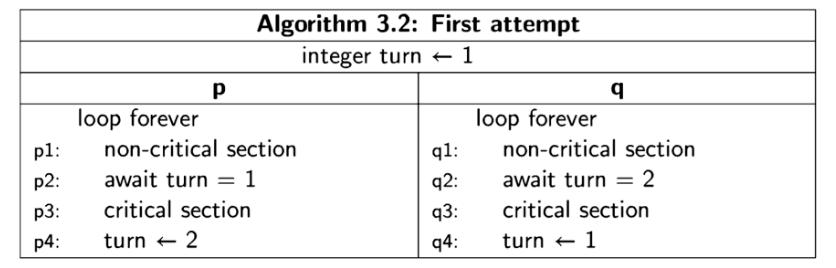
\includegraphics[width=1\textwidth]{3.2.png}\end{center}
Questo primo algoritmo propone la mutua esclusione tramite una singola variabile \textit{turn} che identifica quale processo tra \textit{p} e \textit{q} può accedere alla regione critica.
\newpage
\subsection{Rete di Petri}
In questo particolare caso è stato possibile effettuare una composizione Name-based (Figura \ref{FIG:3.2PN}).
\begin{figure*}[!ht]
\centering
\makebox[0.95\textwidth][c]{
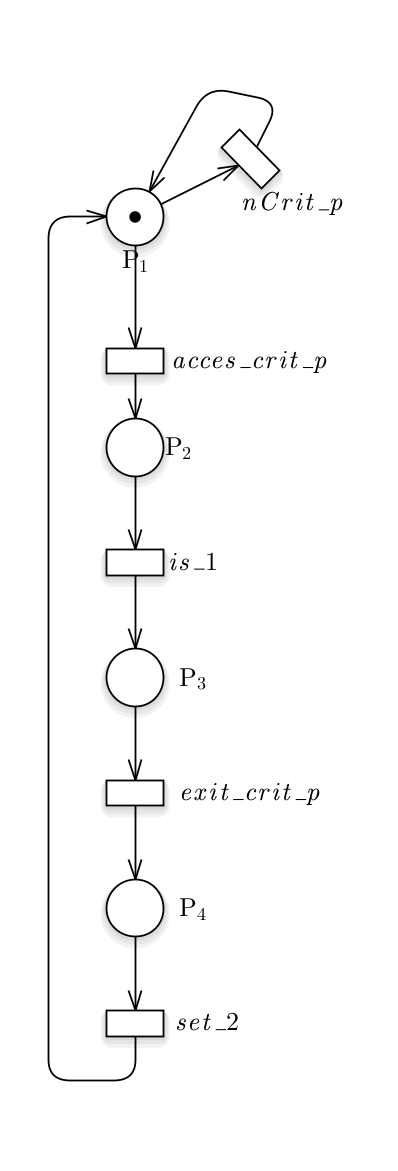
\includegraphics[width=0.5\textwidth]{p3.2.png}
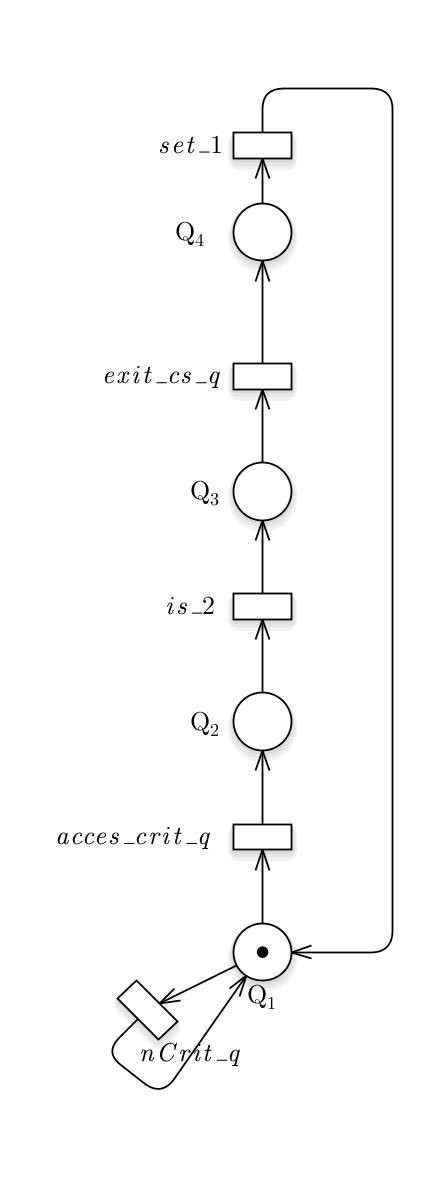
\includegraphics[width=0.5\textwidth]{q3.2.png}
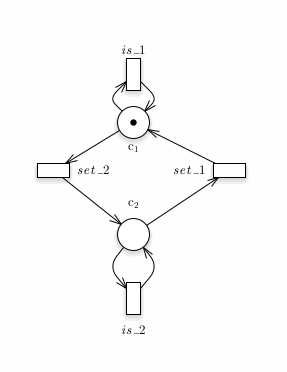
\includegraphics[width=0.5\textwidth]{variable3.2.png}}
\caption{Rete di petri decomposta} \label{FIG:decomposed3.2PN}
\end{figure*}
\begin{figure*}[!ht]
\centering
\makebox[\textwidth][c]{
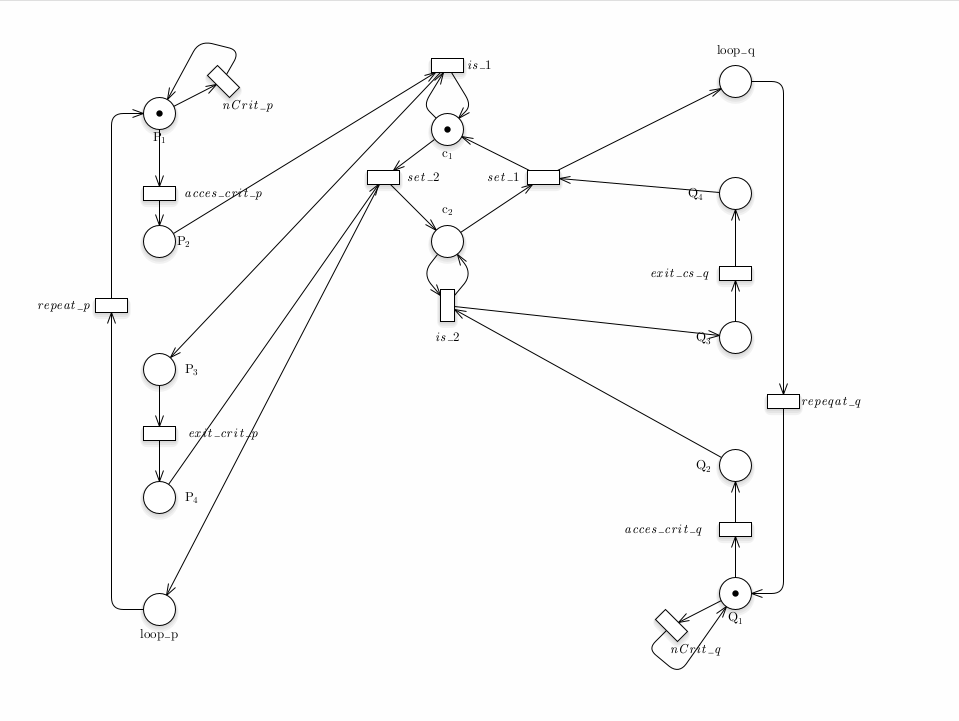
\includegraphics[width=1.5\textwidth]{3.2PN.png}}
\caption{Rete di petri composta} \label{FIG:3.2PN}
\end{figure*}\\
\newpage
\subsubsection{RG}
Il reachability graph, in figura \ref{FIG:3.2RG}, è composto da 16 stati raggiungibili e non presenta alcuno stato di deadlock.
\begin{figure*}[!ht]
\centering
\makebox[\textwidth][c]{
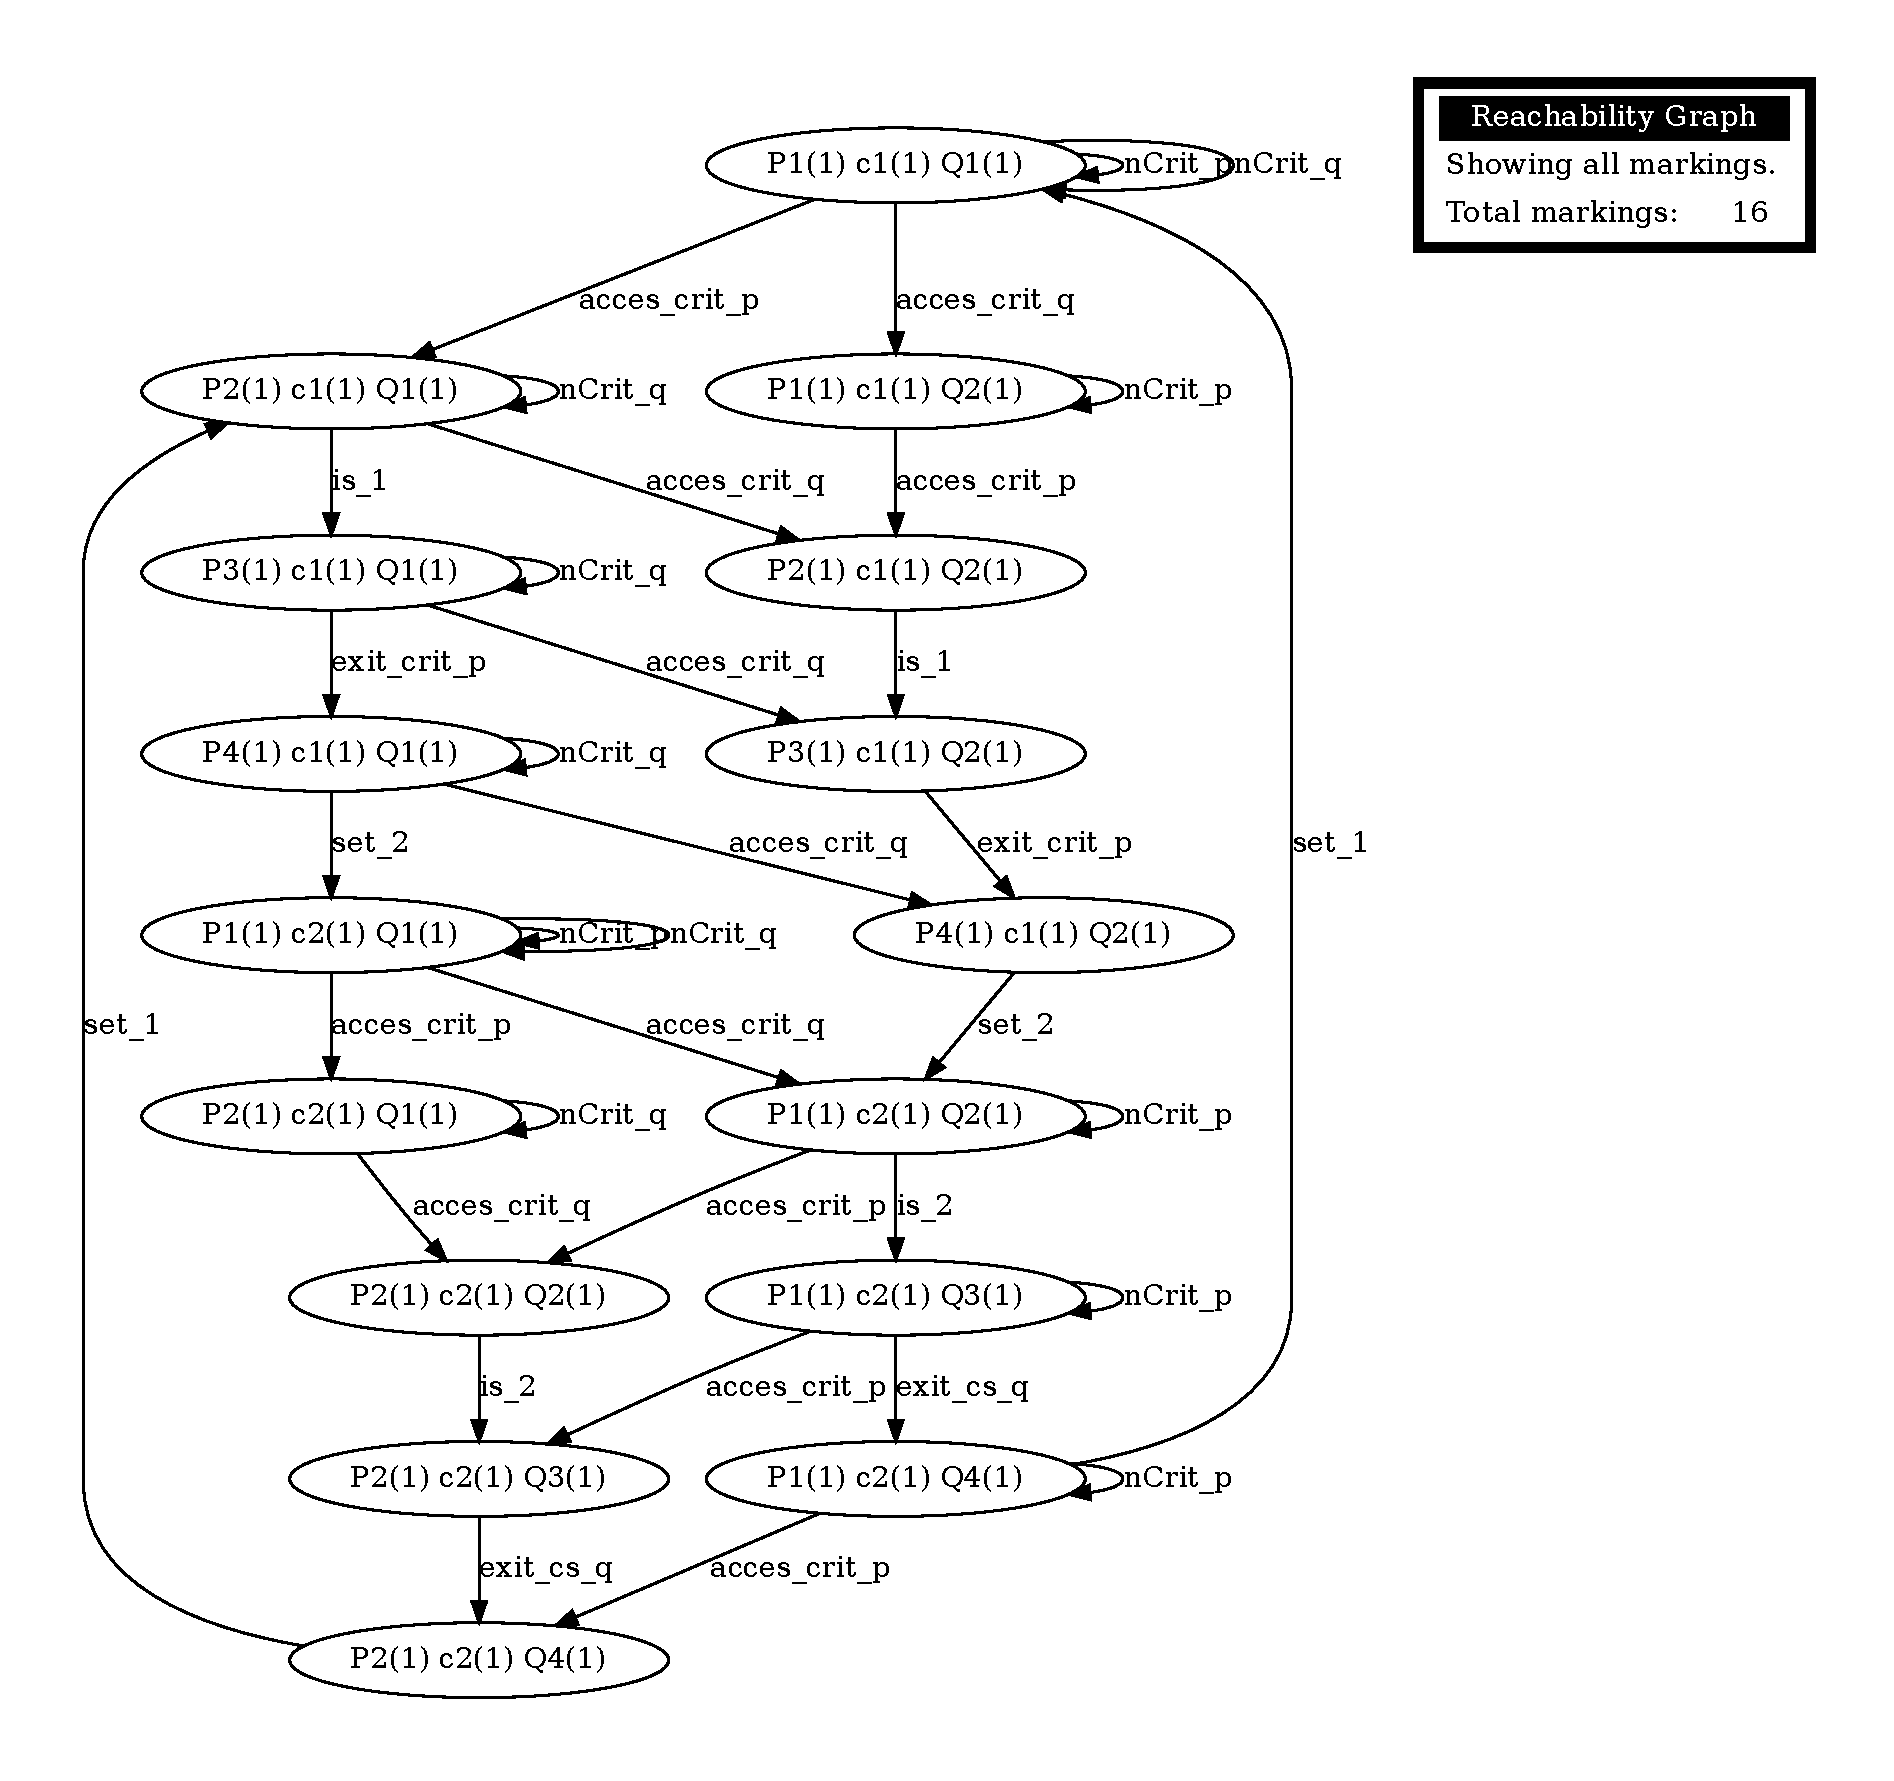
\includegraphics[width=1.5\textwidth]{3.2RG}}
\caption{Reachability graph 3.2} \label{FIG:3.2RG}
\end{figure*}
\newpage
\subsubsection{Analisi strutturale}
Il calcolo dei \textit{semiflow} fornisce 3 \textit{T-semiflow} minimali e 3 \textit{P-semiflow} minimali, i 3 \textit{P-semiflow} permettono di produrre dei P-invarianti e di studiare la boundedness, che in questo caso rivela che tutti i posti sono 1-bound.
Invece dallo studio dei \textit{T-semiflow} si può affermare che il sistema possiede la proprietà di \textit{liveness} in quanto è possibile individuare una \textit{firing sequence} attivabile dalla marcatura iniziale che riporta ad una situazione analoga alla situazione iniziale.\\
2 \textit{T-semiflow} interessanti sono quelli che interessano il posto $P_1$ ed il posto  $Q_1$ in quanto rappresentano una completa esecuzione della $ncs$.\\
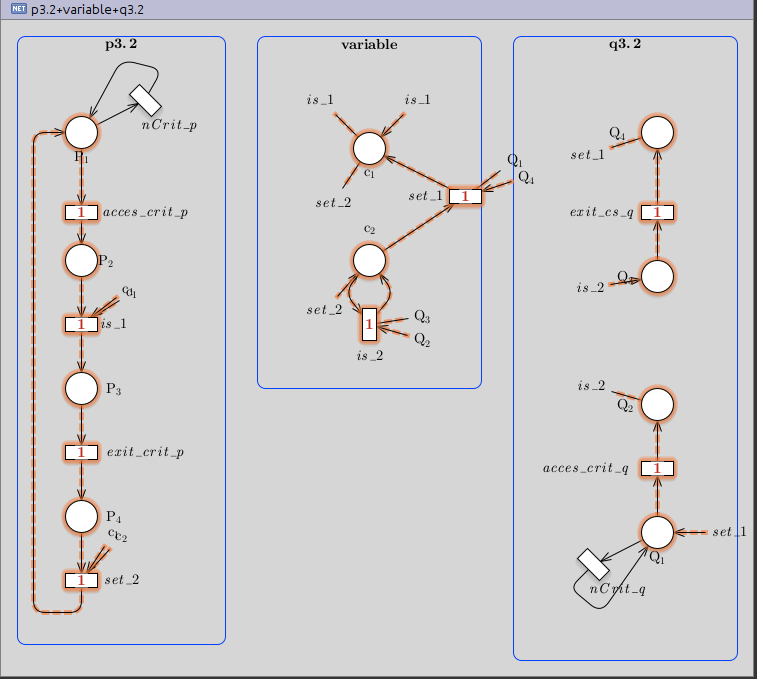
\includegraphics[width=1\textwidth]{3.2T.png}
\newpage
\subsubsection{Model Checking GreatSPN}
Sono state verificate le seguenti formule CTL:
\begin{itemize}
	\item mutua esclusione: \textit{AG !(\#P3==1 \&\& \#Q3==1)} \textcolor{green}{true}.
	\item assenza di starvation: \textit{AG((\#P2 >0 ) -> (AF i\#P3>0 ))} ed anche \textit{AG((\#P2 >0 ) -> (AF i\#P3>0 ))}. Entrambe risultano \textcolor{red}{false}.\\
		Anche inserendo i fairness constrain \textit{\#P1 >0 \textit{e} \#Q1 >0} non è garantita l'assenza di starvation. Il model checker fornisce come controprova il caso in cui \textit{P} è fermo al posto 2, la variabile \textit{turn} vale 2 e \textit{Q} cicla all'infinito in sezione non critica.\\
		L'unico constrain che garantirebbe l'assenza di starvation sarebbe \textit{\#P2 >0 \textit{e} \#Q2 >0} cioè l'imposizione di progresso in regione non critica, in quanto obbligherebbe il processo \textit{Q} a richiedere la sezione critica e modificare il valore della variabile turn.
	\item deadlock: \textit{AG AF ((\#P1==1) || (\#Q1 == 1))} \textcolor{green}{true}. Come ci aspettavamo dalle analisi strutturali e dal DG il sistema non va in deadlock.
\end{itemize}
Sono state verificate le seguenti formule LTL:
\begin{itemize}
	\item mutua esclusione: \textit{G !(\#P3==1 \&\& \#Q3==1)} \textcolor{green}{true}.
	\item assenza di starvation: \textit{G F (\#P2==1) -> G F(\#P3 == 1)} ed anche \textit{G F (\#Q2==1) -> G F(\#Q3 == 1)}. Entrambe risultano \textcolor{red}{false}.
	\item deadlock: \textit{G F( (\#P1 ==1) ||  (\#Q1 ==1))} \textcolor{green}{true}.
\end{itemize}

\subsection{Algebra dei processi}
La codifica del sistema in CCS risulta essere: 
\begin{flalign*}
	&SYS = (P_1 || Q_1 || T_1) /_{\{isT_1, setT_1, isT_2, setT_2\} }&&\\
	&P_1=ncsP.P_1 + ncsP.P_2&&\\
	&P_2=isT_1.P_3&&\\
	&P_3=csP.P_4&&\\
	&P_4=setT_2.P_4&&\\
	&Q_1=ncsQ.Q_1 + ncsQ.Q_2&&\\
	&Q_2=isT_2.Q_3&&\\
	&Q_3=csQ.Q_4&&\\
	&Q_4=setT_1.Q_4&&\\\\
	&T_1=\overline{isT_1}.T_1 + \overline{setT_2}.T_2&&\\
	&T_1=\overline{isT_2}.T_2 + \overline{setT_1}.T_1&&\\
\end{flalign*}
Da cui segue il seguente derivation graph (in cui la riduzione è omessa per chiarezza).\\
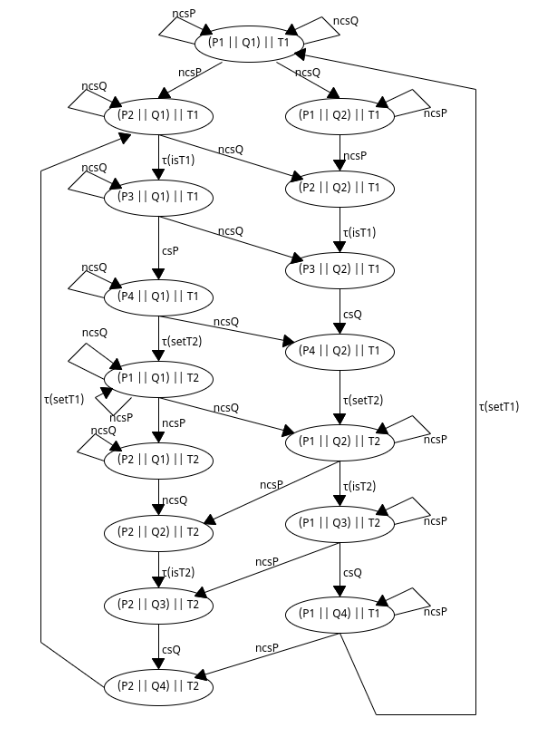
\includegraphics[width=1\textwidth]{3.2CCS.png}\\
Come si può notare il \textit{DG} è composto da 16 stati, esattamente il numero di stati raggiungibili del Reachability Graph, questo è un risultato aspettato in linea con quanto analizzato nelle corrispondenti parti dell'esercizio produttore-consumatore.

\subsection{NuSMV}
L'implementazione del sistema tramite il linguaggio di NuSMV sfrutta la similarità che c'è tra il processo P ed il processo Q.
Infatti i due programmi svolgono le stesse identiche operazioni, ma su variabili differenti, quindi basta dichiare i processi andando ad inserire correttamente i parametri.
Ad esempio il processo p avrà 4 stati: lo stato s1 da cui potrà proseguire richiedendo la sezione critica, oppure rimanendo in s1, lo stato s3 che corrisponde alla sezione critica e lo stato s4 che corrisponde all'uscita dalla sezione critica ed la ripetizione del programma completo.\\
Più interessante è lo stato s4, dove si nota il riuso del codice. 
Per poter accede alla sezione critica il turno deve essere 1, quindi il processo P va a confrontare il valore della variabile \textit{turn} con lo il valore della variabile \textit{var\_wait} che in questo caso è 1, se corrispondono il programma prosegue in s3.
Operazione simile viene effettuata quando P va ad impostare il valore della variabile \textit{turn} in uscita dalla sezione critica.
\lstinputlisting{figures/3_2_code.smv}
Il comando \texttt{print\_reachable\_states} mostra 16 stati raggiungibili di 32 possibili, in linea con la dimensione del Derivation Graph e del Reachability Graph.
Tra tutti gli stati raggiungibili non è presente alcuno stato di Deadlock.

\newpage
\subsubsection{Model Checking NuSMV}
Sono state verificate le seguenti formule CTL:
\begin{itemize}
        \item mutua esclusione: \textit{AG !(( p.state = s3 ) \& (q.state = s3 ))} \textcolor{green}{true}.
        \item assenza di starvation: \textit{AG (( p.state = s2 ) -> (AF p.state = s3 ))} ed anche \textit{AG (( q.state = s2 ) -> (AF q.state = s3 ))}. Entrambe risultano \textcolor{red}{false}.\\
                Anche inserendo il fairness constrain \textit{FAIRNESS running} non è garantita l'assenza di starvation. Il model checker fornisce come controprova il caso in cui p è fermo allo stato s2, la variabile turn vale 2 e q cicla all'infinito in sezione non critica. Viene data la possibilità al processo p di eseguire il suo codice, ma essendo $turn = 2$ questi non può entrare in regione critica.
        \item deadlock: \textit{AG AF (( p.state = s1 )| ( q.state = s1 ))} \textcolor{green}{true}. Come ci aspettavamo dalle analisi strutturali e dal DG il sistema non va in deadlock.
\end{itemize}
Sono state verificate le seguenti formule LTL:
\begin{itemize}
        \item mutua esclusione: \textit{G !(p.state = s3 \& q.state = s3)} \textcolor{green}{true}.
        \item assenza di starvation: \textit{G (p.state = s2 ->  F p.state = s3)} ed anche \textit{G (p.state = s2 ->  F p.state = s3)}. Entrambe risultano \textcolor{red}{false}.\\
		Anche inserendo il fairness constrain \textit{FAIRNESS running} non è garantita l'assenza di starvation. Il model checker fornisce come controprova un caso più lungo del necessario in cui comunque alla fine ci si riconduce alla situazione in cui p è fermo allo stato s2, la variabile turn vale 2 e q cicla all'infinito in sezione non critica.
        \item deadlock: \textit{G F(( p.running) | ( q.running ) )} \textcolor{red}{false}. In questo caso sembra verificarsi deadlock, perchè esiste una esecuzione in cui solo il processo Main viene eseguito.\\
		Quindi il problema non è tanto la presenza di deadlock quanto l'incapacità di scrivere la formula in modo da tenere conto anche dell'esecuzione del processo Main. Non riuscendo a rifermi al modulo main dall'interno del main stesso ho "risolto" imponendo \textit{FAIRNESS running}.
\end{itemize}

\newpage
\section{Algoritmo 3.6}
\label{SEC:3.6}
\begin{center}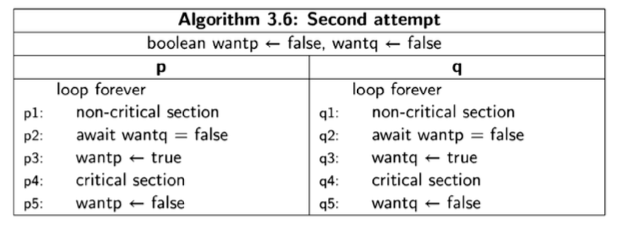
\includegraphics[width=1\textwidth]{3.6.png}\end{center}
Questo algoritmo propone la mutua esclusione tramite due variabili \textit{wantp \textit{e} wantq} che indicano se un processo vuole entrare in sezione critica. Un processo può entrare in sezione critica solamente se l'altro non vuole. quando il processo entra in sezione critica imposta la variabile relativa a lui a true. 
\subsection{Rete di Petri}
\newpage
\begin{center}
\makebox[\textwidth][c]{
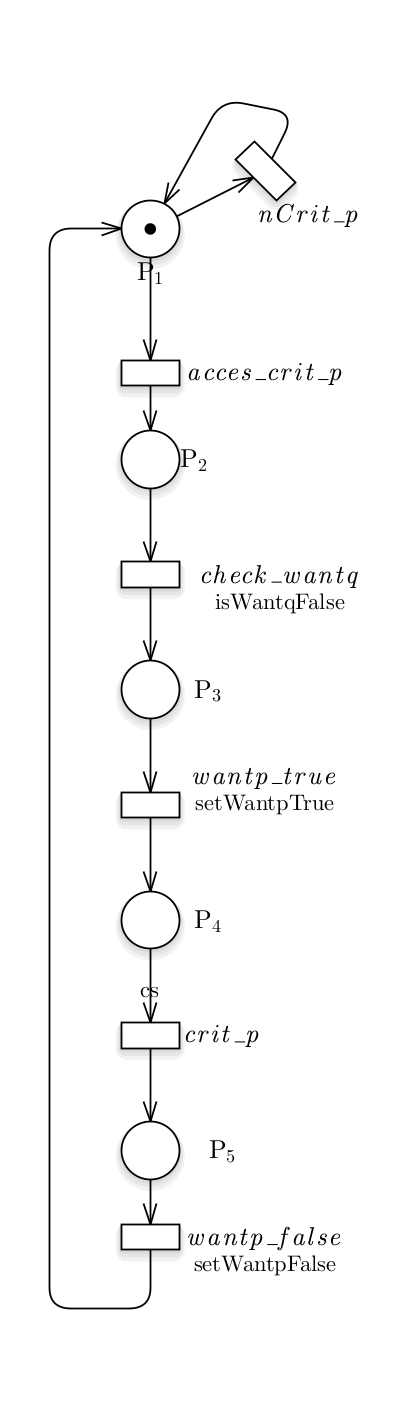
\includegraphics[width=0.34\textwidth]{p3.6.png}
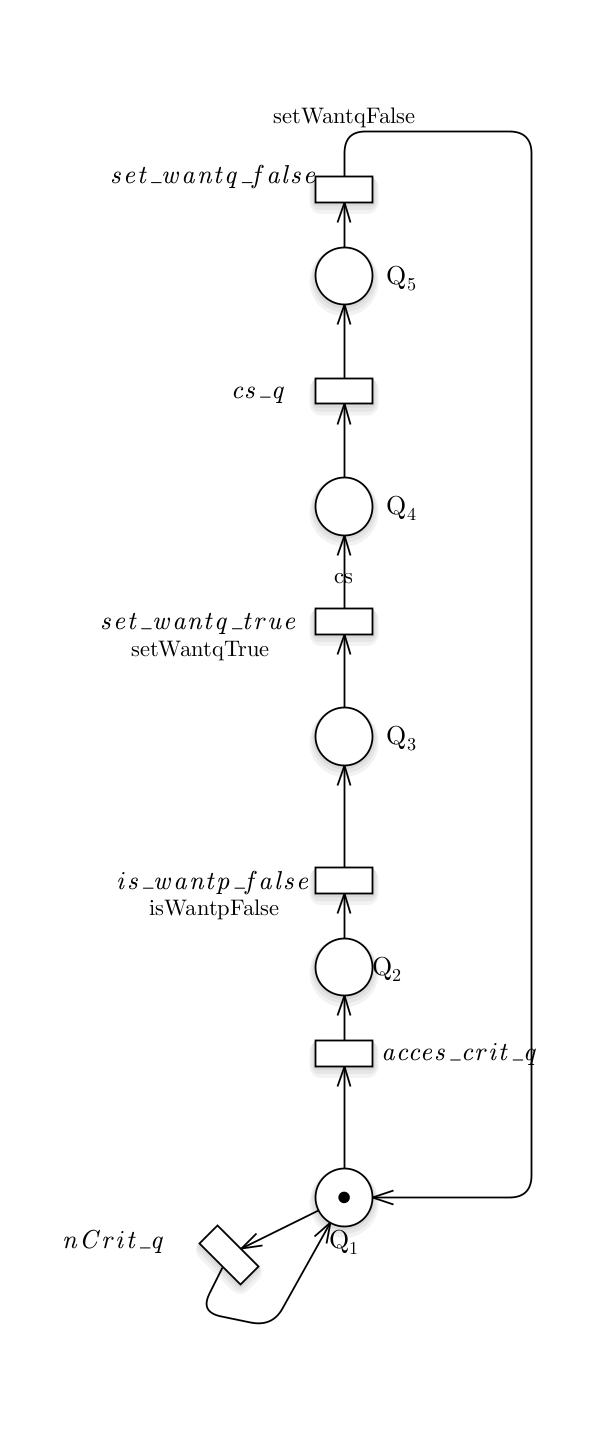
\includegraphics[width=0.5\textwidth]{q3.6.png}
}
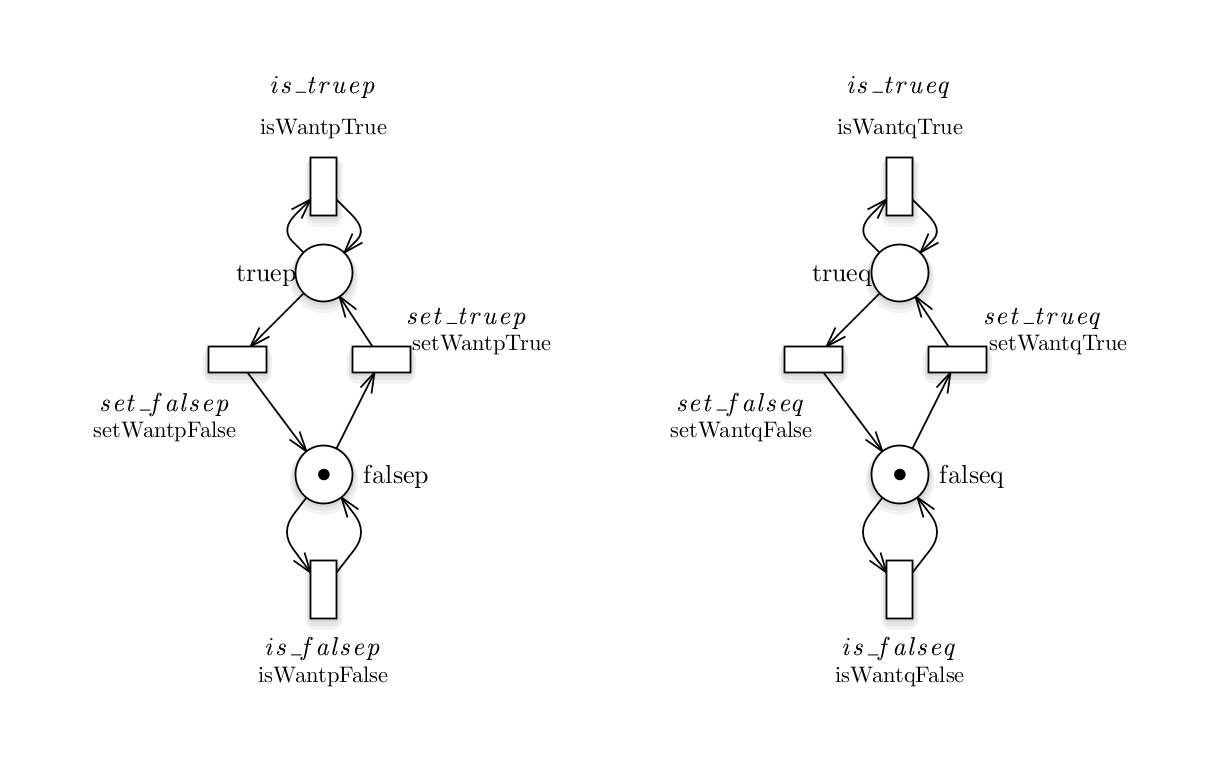
\includegraphics[width=0.8\textwidth]{variables.png}
\end{center}
\newpage
\begin{figure*}[!ht]
\centering
\makebox[\textwidth][c]{
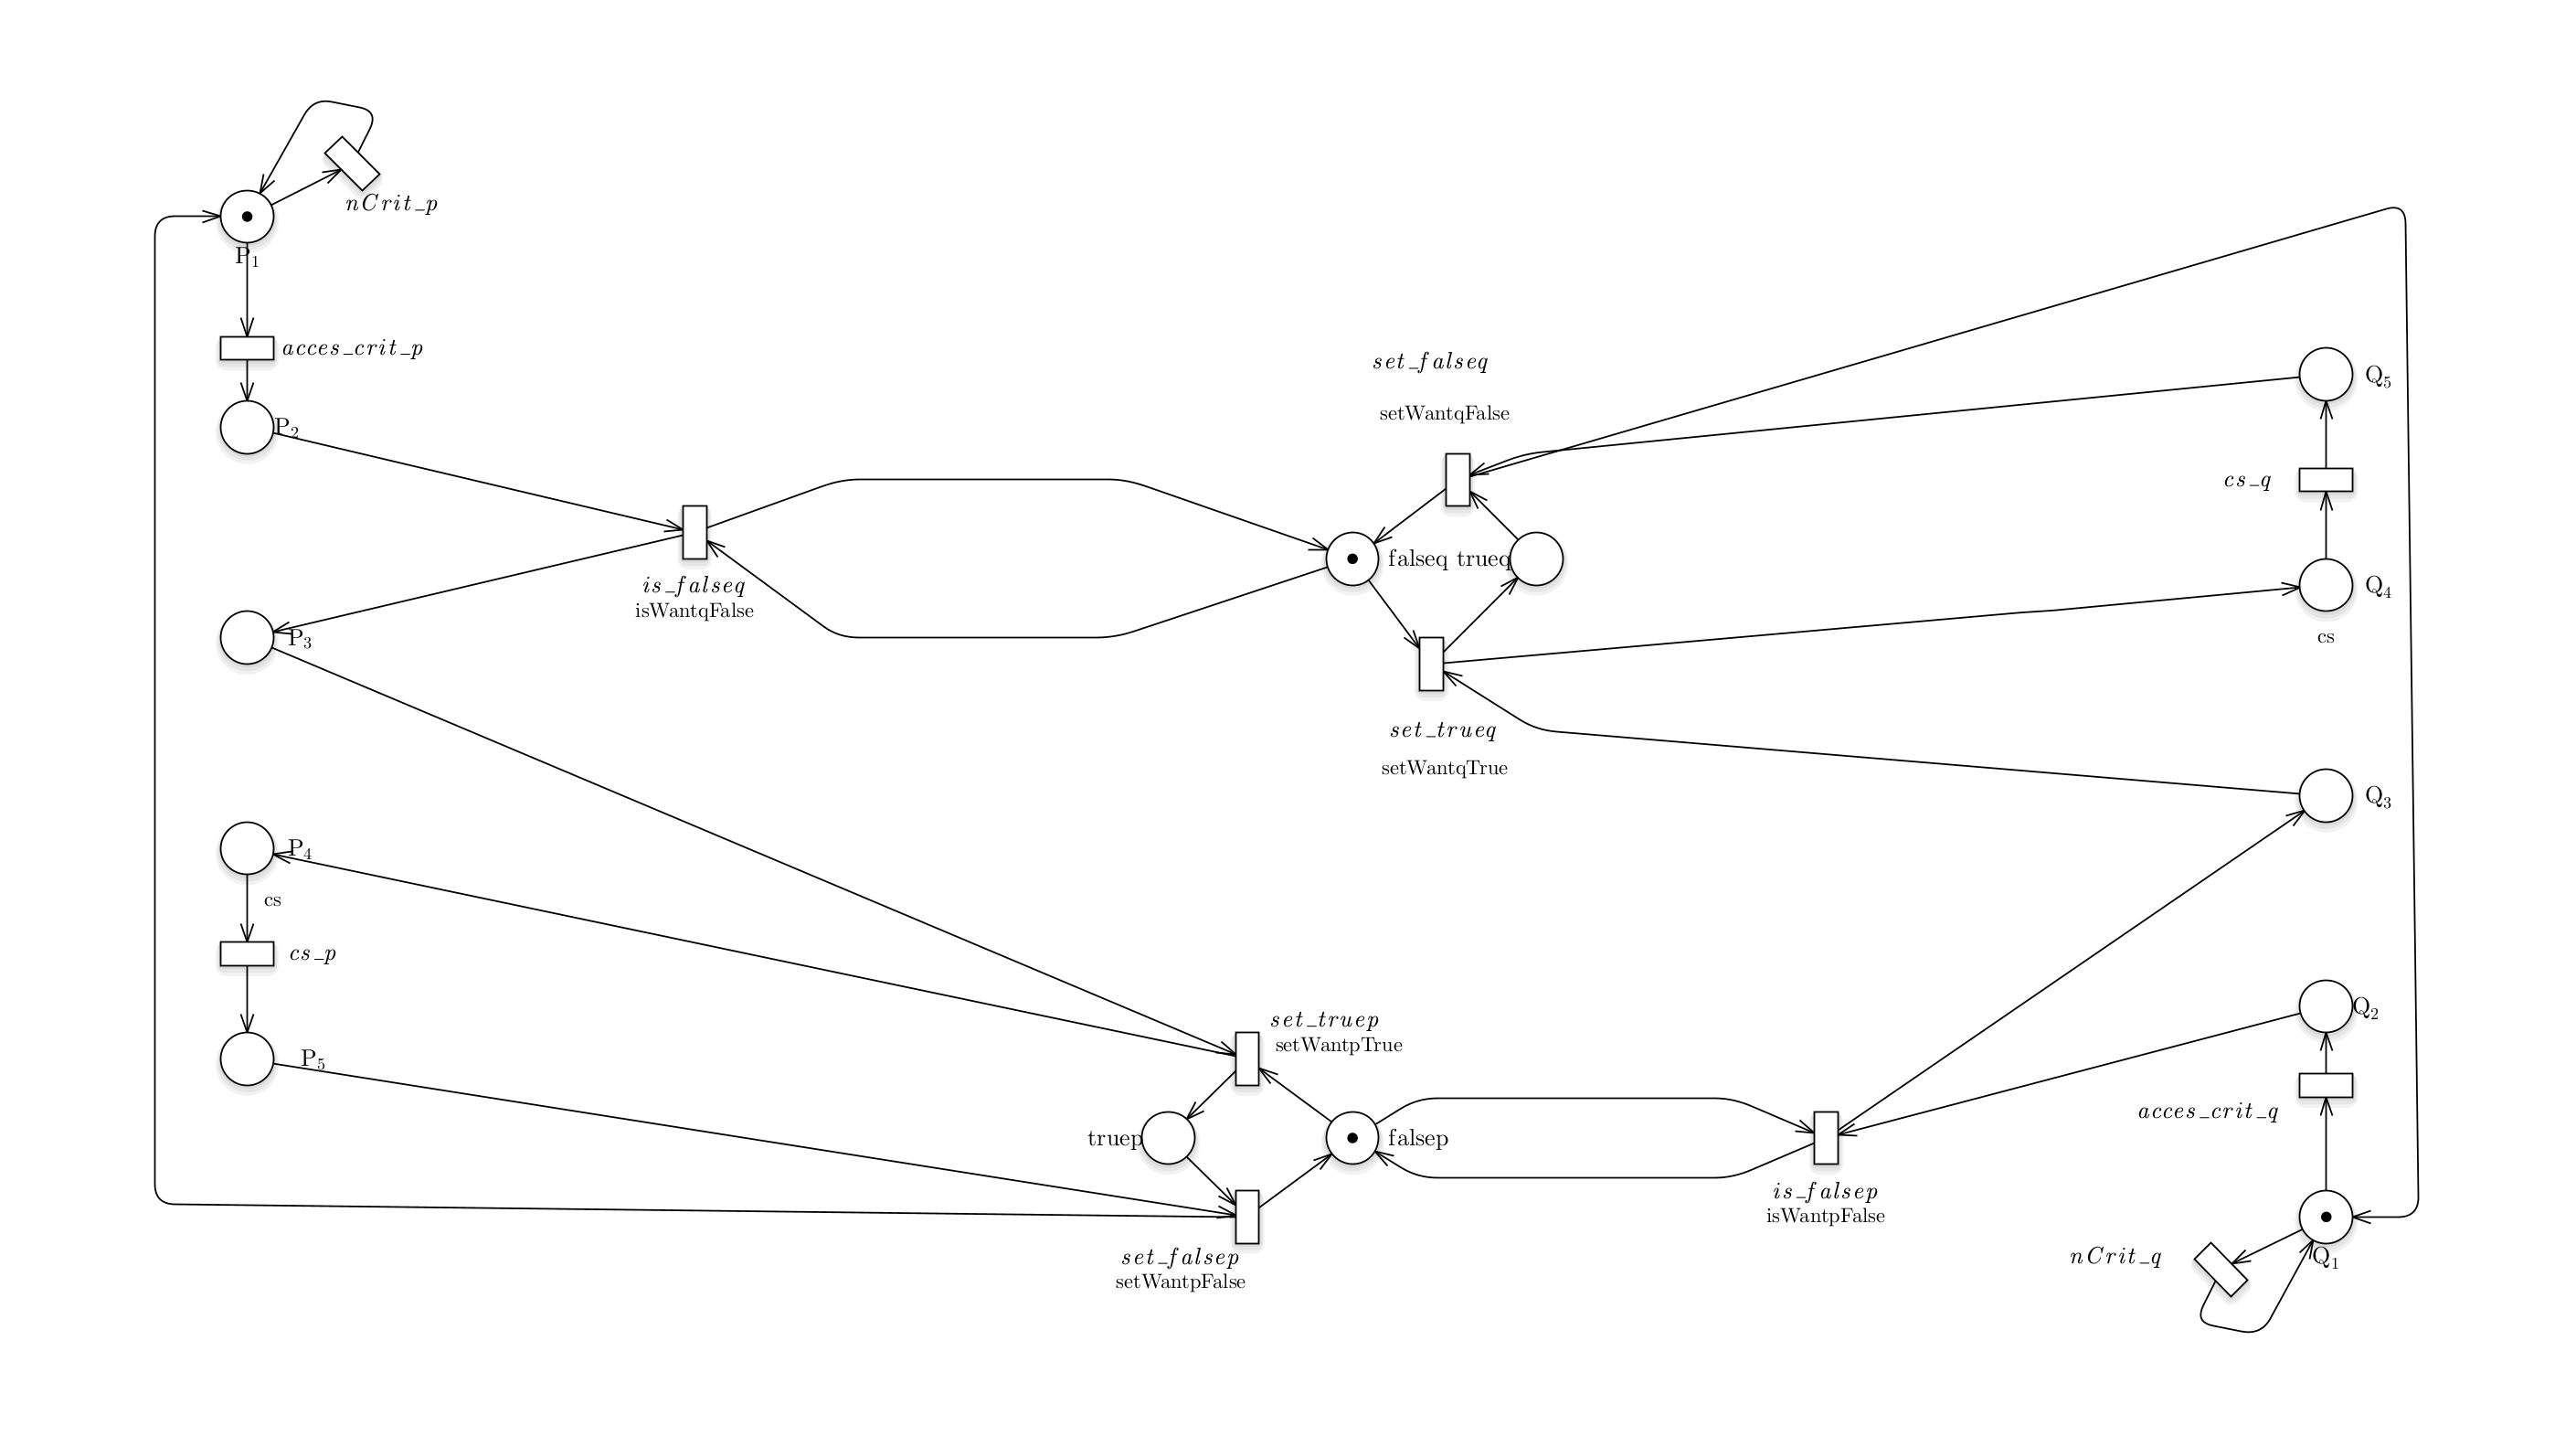
\includegraphics[width=1.6\textwidth]{3.6PN.png}}
\caption{Rete di petri composta} \label{FIG:3.6PN}
\end{figure*}
\newpage
\subsubsection{RG}
Il reachability graph, in figura \ref{FIG:3.6RG}, è composto da 25 stati raggiungibili e non presenta alcun deadlock.
\begin{figure*}[!ht]
\centering
\makebox[\textwidth][c]{
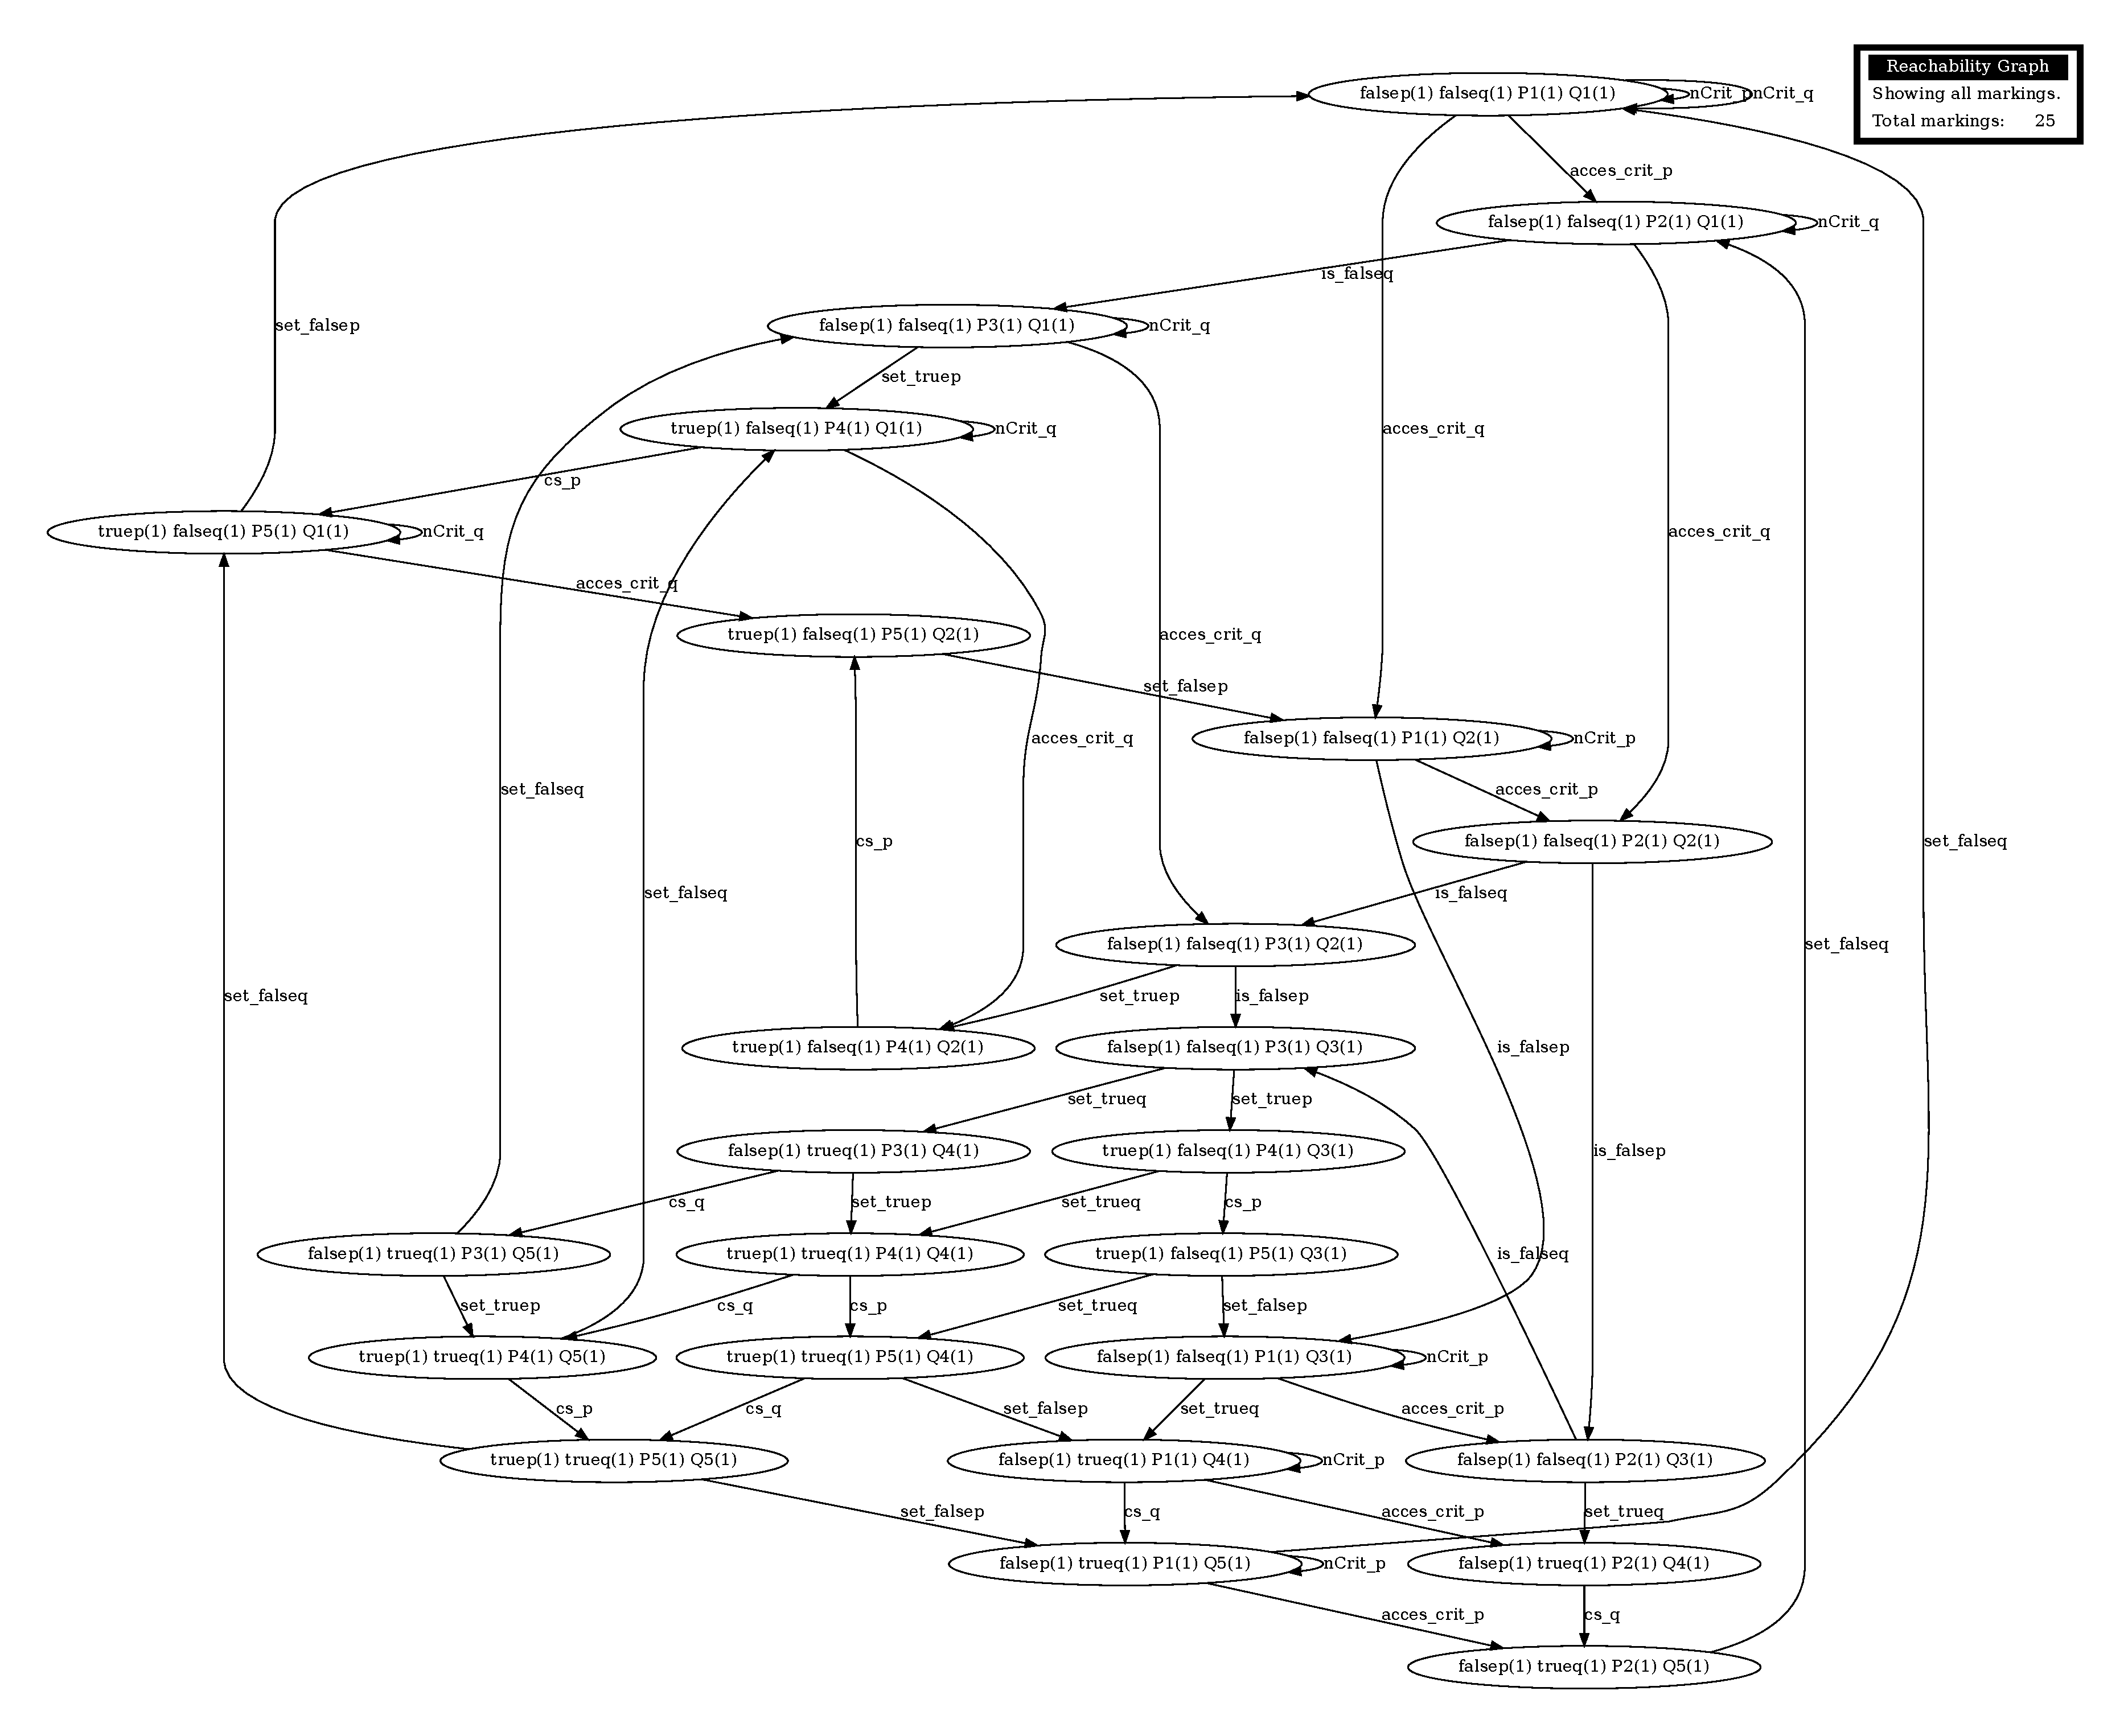
\includegraphics[width=1.5\textwidth]{3.6RG}}
\caption{Reachability graph 3.6} \label{FIG:3.6RG}
\end{figure*}
\newpage
\subsubsection{Analisi strutturale}
\label{SEC:3_8_strutturale}
Il calcolo dei \textit{semiflow} fornisce 4 \textit{T-semiflow} minimali e 8 \textit{P-semiflow} minimali, gli 8 \textit{P-semiflow} permettono di produrre dei P-invarianti e di studiare la boundedness, che in questo caso rivela che tutti i posti sono 1-bound.\\
I \textit{T-semiflow} garantiscono che le due variabili \texttt{falseq \texttt{e} faslep} non assumono mai contemporaneamente il valore di vero e di falso e che ogni processo è sempre in esattamente un solo valore di program counter.

\subsubsection{Model Checking GreatSPN}
Sono state verificate le seguenti formule CTL:
\begin{itemize}
	\item mutua esclusione: \textit{AG !(\#P4==1 \&\& \#Q4==1)} \textcolor{red}{false}.\\
		Il model checker fornisce come controesempio l'esecuzione \\$\{P_1 Q_1,P_1 Q_2,P_2 Q_2,P_2 Q_3,P_3 Q_3,P_3 Q_4,P_4 Q_4\}$.
	\item assenza di starvation: \textit{AG((\#P2 >0 ) -> (AF \#P4>0 ))} ed anche \textit{AG((\#P2 >0 ) -> (AF \#P4>0 ))}. Entrambe risultano \textcolor{red}{false}.\\
		In questo caso risulta più complicato inserire dei \textit{fairness constraint} sensati. Infatti l'assenza di starvation dipende moltissimo dallo scheduling utilizzato.  
		Inserendo il fairness constrain più "elmentare", \textit{\#P1 >0 \textit{e} \#Q1 >0} cioè "viene quantomeno fornito tempo di CPU al processo p" , non è garantita l'assenza di starvation. Il model checker fornisce come controprova il caso in cui \textit{P} è fermo al posto 2, e viene solo eseguito \textit{Q} che cicla all'infinito in sezione non critica.\\
		Un altro constrain che garantirebbe l'assenza di starvation sarebbe \textit{\#P2 >0 \textit{e} \#Q2 >0} cioè l'imposizione di progresso in regione non critica.%TODO: non è vero e non capisco perchè
	\item deadlock: \textit{AG AF ((\#P1==1) || (\#Q1 == 1))} \textcolor{green}{true}. Come ci aspettavamo dalle analisi strutturali e dal DG il sistema non va in deadlock.
\end{itemize}
Sono state verificate le seguenti formule LTL:
\begin{itemize}
	\item mutua esclusione: \textit{G !(\#P4==1 \&\& \#Q4==1)} \textcolor{red}{false}.
	\item assenza di starvation: \textit{G F (\#P2==1) -> G F(\#P4 == 1)} ed anche \textit{G F (\#Q2==1) -> G F(\#Q4 == 1)}. Entrambe risultano \textcolor{red}{false}.
	\item deadlock: \textit{G F( (\#P1 ==1) ||  (\#Q1 ==1))} \textcolor{green}{true}.
\end{itemize}

\subsection{Algebra dei processi}
La codifica del sistema in CCS risulta essere: 
\begin{flalign*}
	&SYS = (P_1 || Q_1 || noWantP || noWantQ) /_{\{falseWp,falseWq,trueWp,trueWq,notWp,notWq\} }&&\\
	&P_1=ncsP.P_1 + ncsP.P_2&&\\
	&P_2=notWq.P_3&&\\
	&P_3=trueWp.P_4&&\\
	&P_4=csP.P_4&&\\
	&P_5=falseWp.P_1&&\\
	&Q_1=ncsP.P_1 + ncsP.P_2&&\\
	&Q_2=notWp.P_3&&\\
	&Q_3=trueWq.P_4&&\\
	&Q_4=csP.P_4&&\\
	&Q_5=falseWq.P_1&&\\\\
	&WantP=\overline{falseWp}.noWantP&&\\
	&noWantP=\overline{notWp}.noWantP + \overline{trueWp}.WantP &&\\
	&WantQ=\overline{falseWq}.noWantQ&&\\
	&noWantQ=\overline{notWq}.noWantQ + \overline{trueWq}.WantQ &&\\
\end{flalign*}
Da cui segue il seguente derivation graph.\\
\makebox[\textwidth][c]{
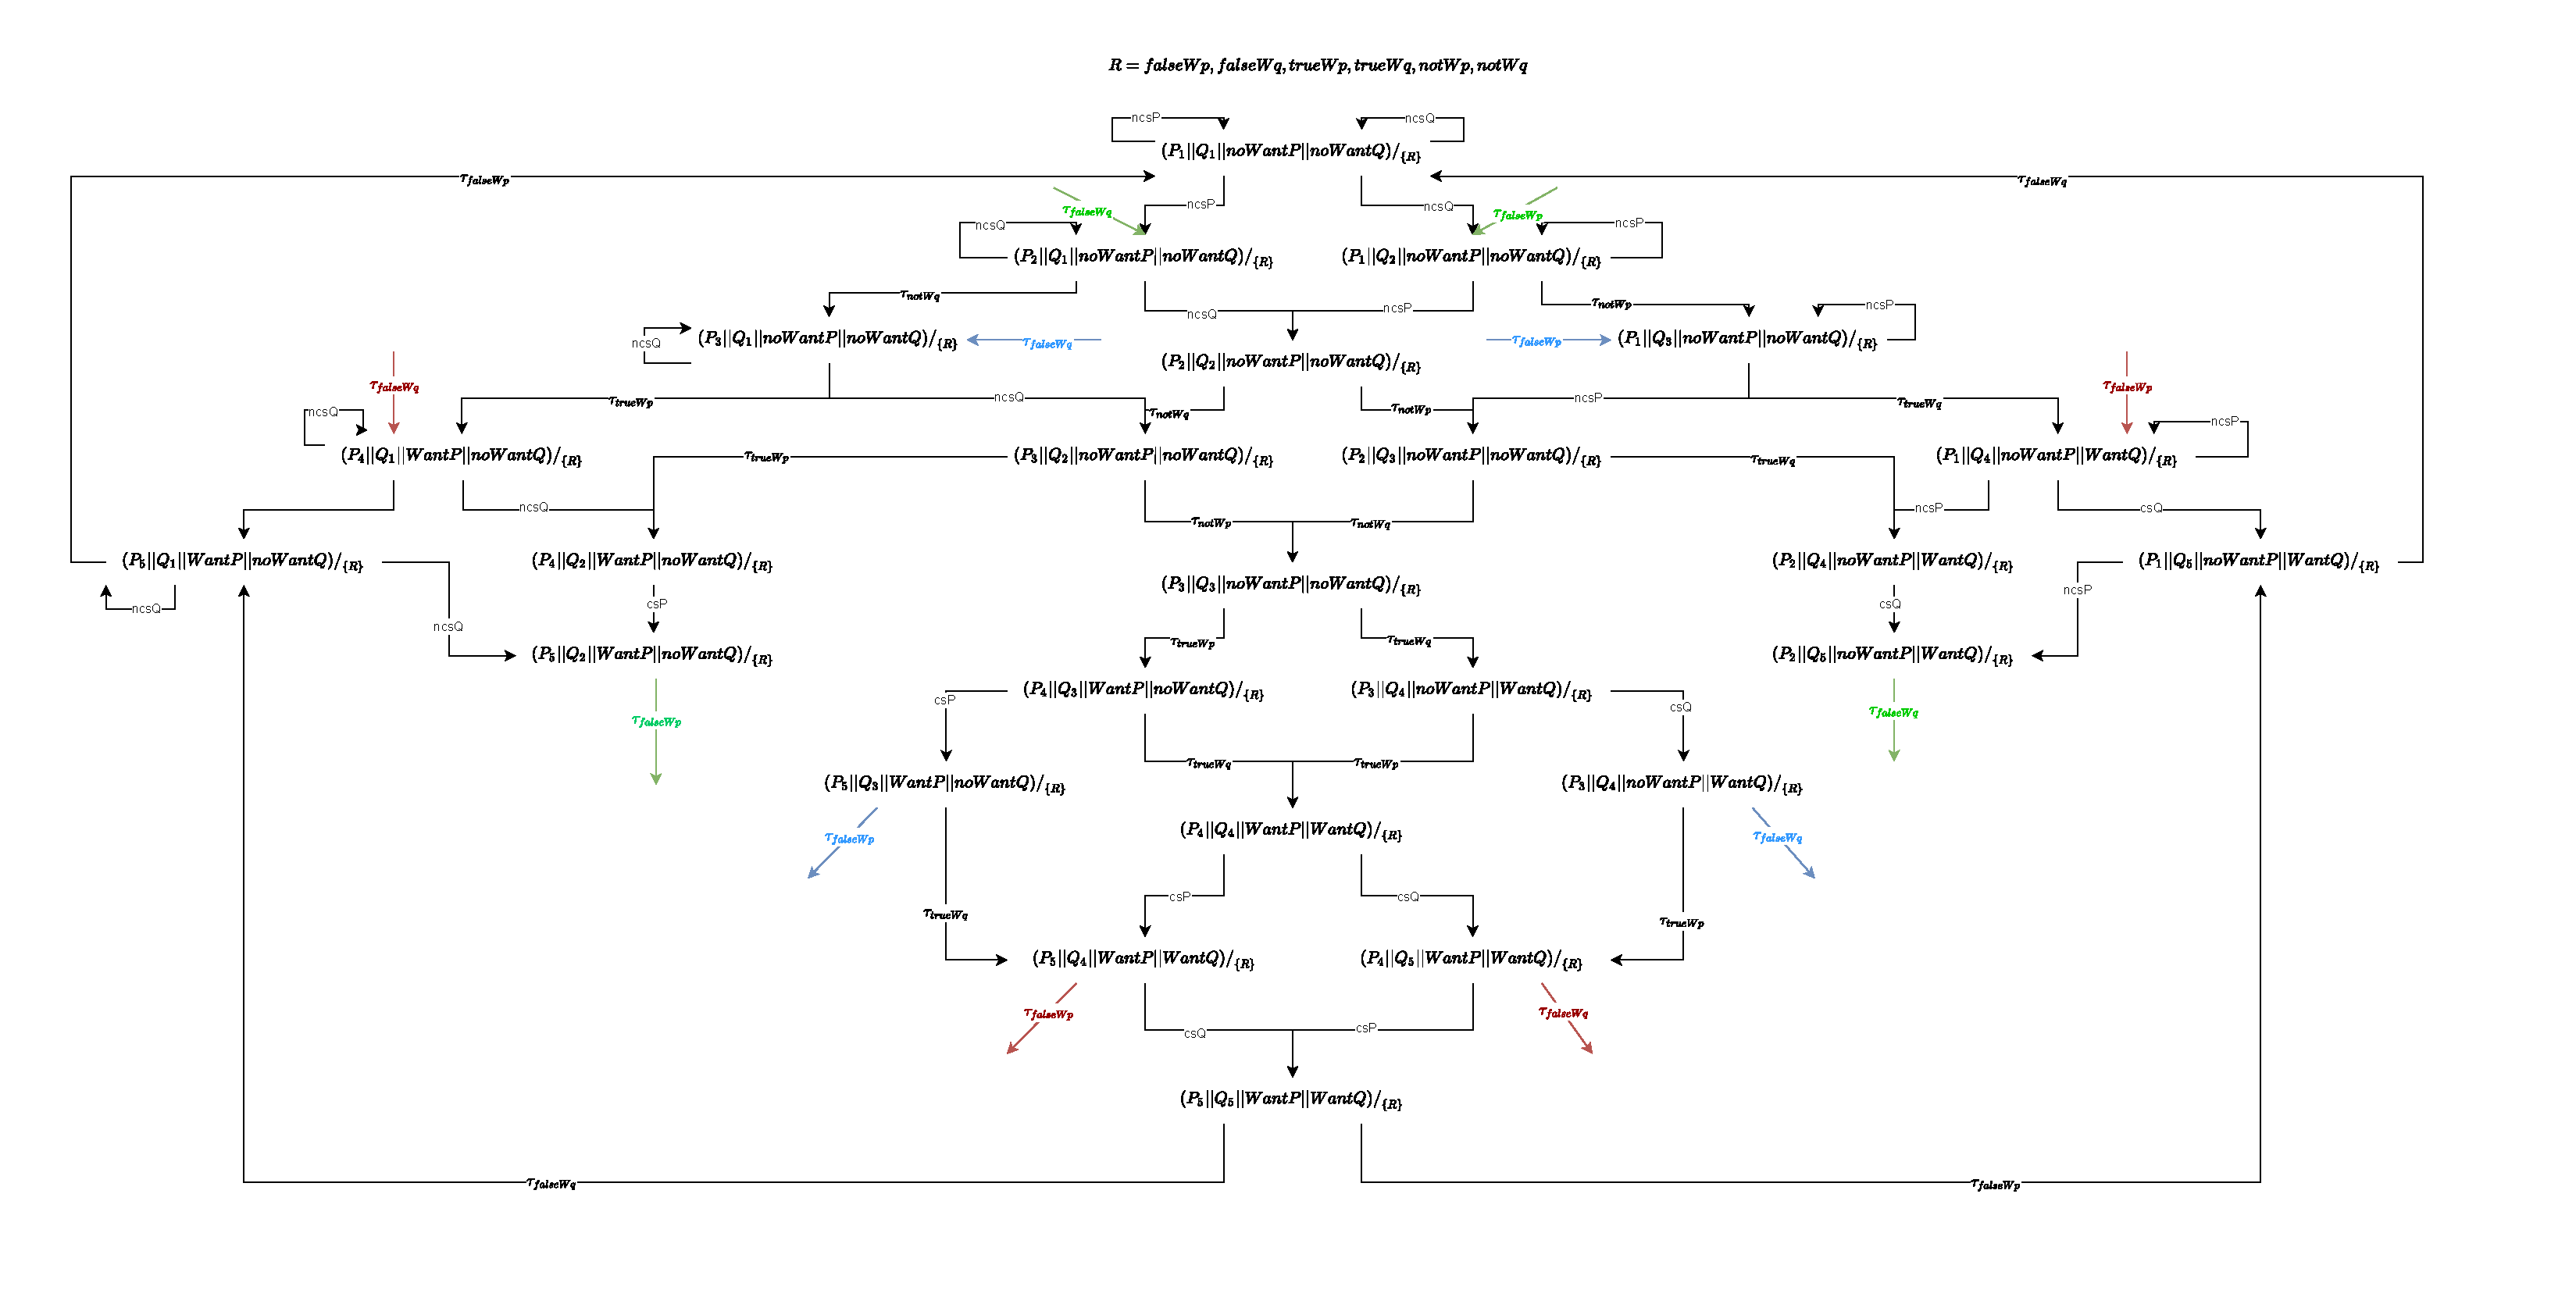
\includegraphics[width=1.5\textwidth]{3_6CCS}}\\
Come si può notare il \textit{DG} è composto da 25 stati, esattamente il numero di stati raggiungibili del Reachability Graph, questo è un risultato aspettato in linea con quanto analizzato nelle corrispondenti parti dell'esercizio produttore-consumatore.

\subsection{NuSMV}
\label{SUBSEC:3.6NuSMV}
L'implementazione del sistema tramite il linguaggio di NuSMV sfrutta la similarità che c'è tra il processo P ed il processo Q, come nel caso precedente.
Questa volta però non è solo una variabile ad essere interessata dallo scambio di parametri, bensì le due variabili \textit{wantp} e \textit{wantq}.\\
Un paragone che rende facilmente intuibile il comportamento dei due moduli è leggere i due parametri come la variabile che indica "io voglio entrare in sezione critica" e "l'altro vuole entrare in sezione critica", ed è per questo che le due variabili sono state chiamate \textit{want\_me \textit{e} want\_other}
Per il resto il riuso del codice è identico al caso precedente.
\lstinputlisting{figures/3_6_code.smv}
Il comando \texttt{print\_reachable\_states} mostra 25 stati raggiungibili di 100 possibili, in linea con la dimensione del Derivation Graph e del Reachability Graph.
Tra tutti gli stati raggiungibili non è presente alcuno stato di Deadlock ma è presente uno stato in cui la mutua esclusione viene violata ($p.state=s4,q.state=s4,wantp=true,wantq=true$).

\subsubsection{Model Checking NuSMV}
Sono state verificate le seguenti formule CTL:
\begin{itemize}
        \item mutua esclusione: \textit{AG !(( p.state = s4 ) \& (q.state = s4 ))} \textcolor{red}{false}.\\
		Il model checker fornisce come controesempio l'esecuione $\{p.state=s1\;q.state=s1,p.state=s1\;q.state=s2,p.state=s2\;q.state=s2,p.state=s2\;q.state=s3,p.state=s3\;q.state=s3,p.state=s3\;q.state=s4,p.state=s4\;q.state=s4\}$.
        \item assenza di starvation: \textit{AG (( p.state = s2 ) -> (AF p.state = s3 ))} ed anche \textit{AG (( q.state = s2 ) -> (AF q.state = s3 ))}. Entrambe risultano \textcolor{red}{false}.\\
		Anche inserendo il fairness constrain \textit{FAIRNESS running} non è garantita l'assenza di starvation. Il model checker fornisce come controprova il caso in cui p è fermo allo stato s2, q esegue un ciclo completo del programma (tornando in s1) e 2 volte viene passata l'esecuzione al processo p. Ma p è bloccato da \textit{wantq} e non può proseguire.\\
		Questo caso specifico fa parte di una più ampia classe di esecuzioni in cui viene concessa l'esecuzione del processo p sempre quando questi è bloccato prima dell'accesso in sezione critica.
        \item deadlock: \textit{AG AF (( p.state = s1 )| ( q.state = s1 ))} \textcolor{green}{true}. Come ci aspettavamo dalle analisi strutturali e dal DG il sistema non va in deadlock.
\end{itemize}
Sono state verificate le seguenti formule LTL:
\begin{itemize}
        \item mutua esclusione: \textit{G !(p.state = s4 \& q.state = s4)} \textcolor{red}{false}.\\
		Come nel caso di CTL il sistema non rispetta la mutua esclusione, il controesempio fornito è lo stesso di CTL.
        \item assenza di starvation: \textit{G (p.state = s2 ->  F p.state = s3)} ed anche \textit{G (p.state = s2 ->  F p.state = s3)}. Entrambe risultano \textcolor{red}{false}.\\
		Anche questo caso fornisce un controesempio identico a quello fornito in fase di analisi con CTL.
        \item deadlock: \textit{G F(( p.running) | ( q.running ) )} \textcolor{red}{false}. 
		Come in sezione \ref{SEC:3.2} si pone di nuovo il problema di fare riferimento al modulo main dall'interno del modulo stesso. Viene sfruttato di nuovo \textit{FAIRNESS running} per ottenere un risultato coerente con l'analisi.
\end{itemize}
\newpage
\section{Confronto tramite bisimulazione tra 3.2 e 3.6}
%TODO: fare equivalenze a tracce, fallimento e simulazione?
Per maggior leggibilità ho modificato i derivation graph dei due algoritmi, identificando con X oppure Y seguiti da un apice lo stato.\\
\begin{figure*}[!ht]
\centering
\makebox[\textwidth][c]{
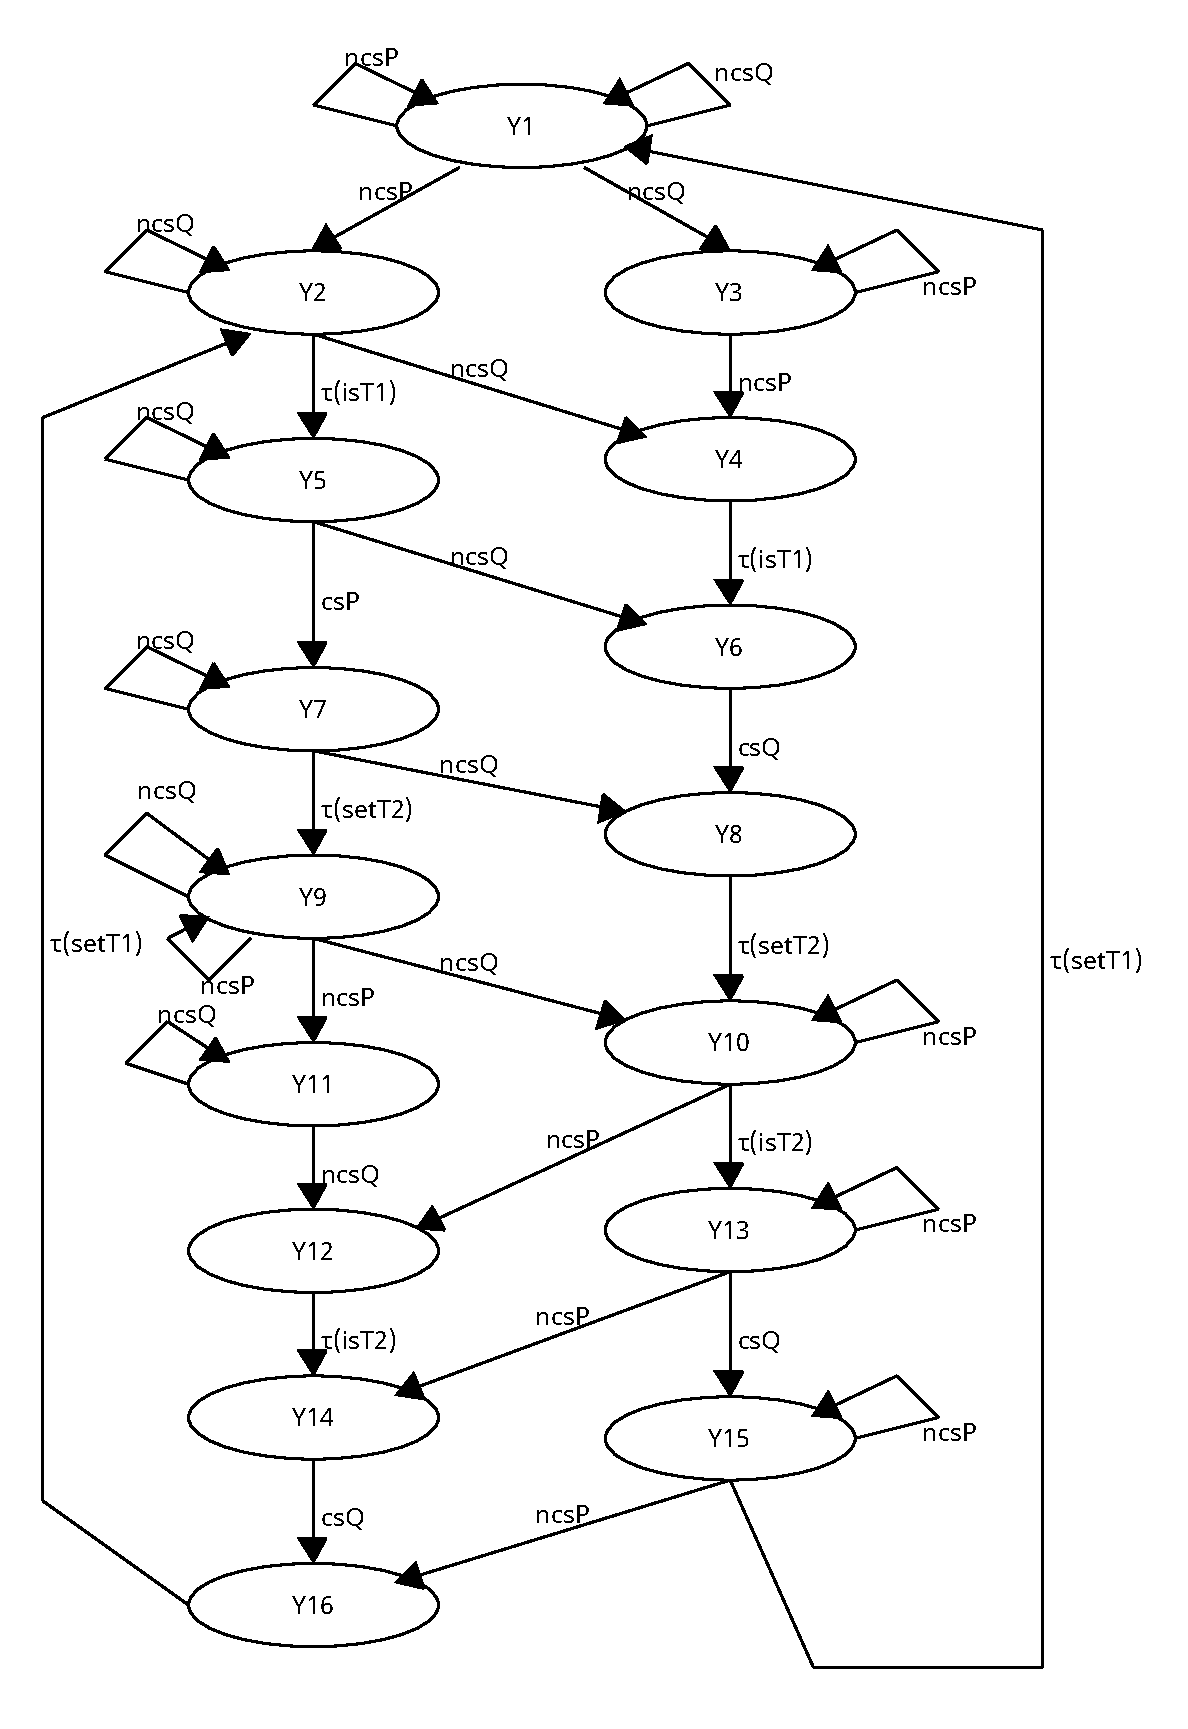
\includegraphics[width=0.5\textwidth]{3_2Eq}}
\caption{Derivation graph 3.2, Y} \label{FIG:3.2Eq}
\end{figure*}\\
\begin{figure*}[!ht]
\centering
\makebox[\textwidth][c]{
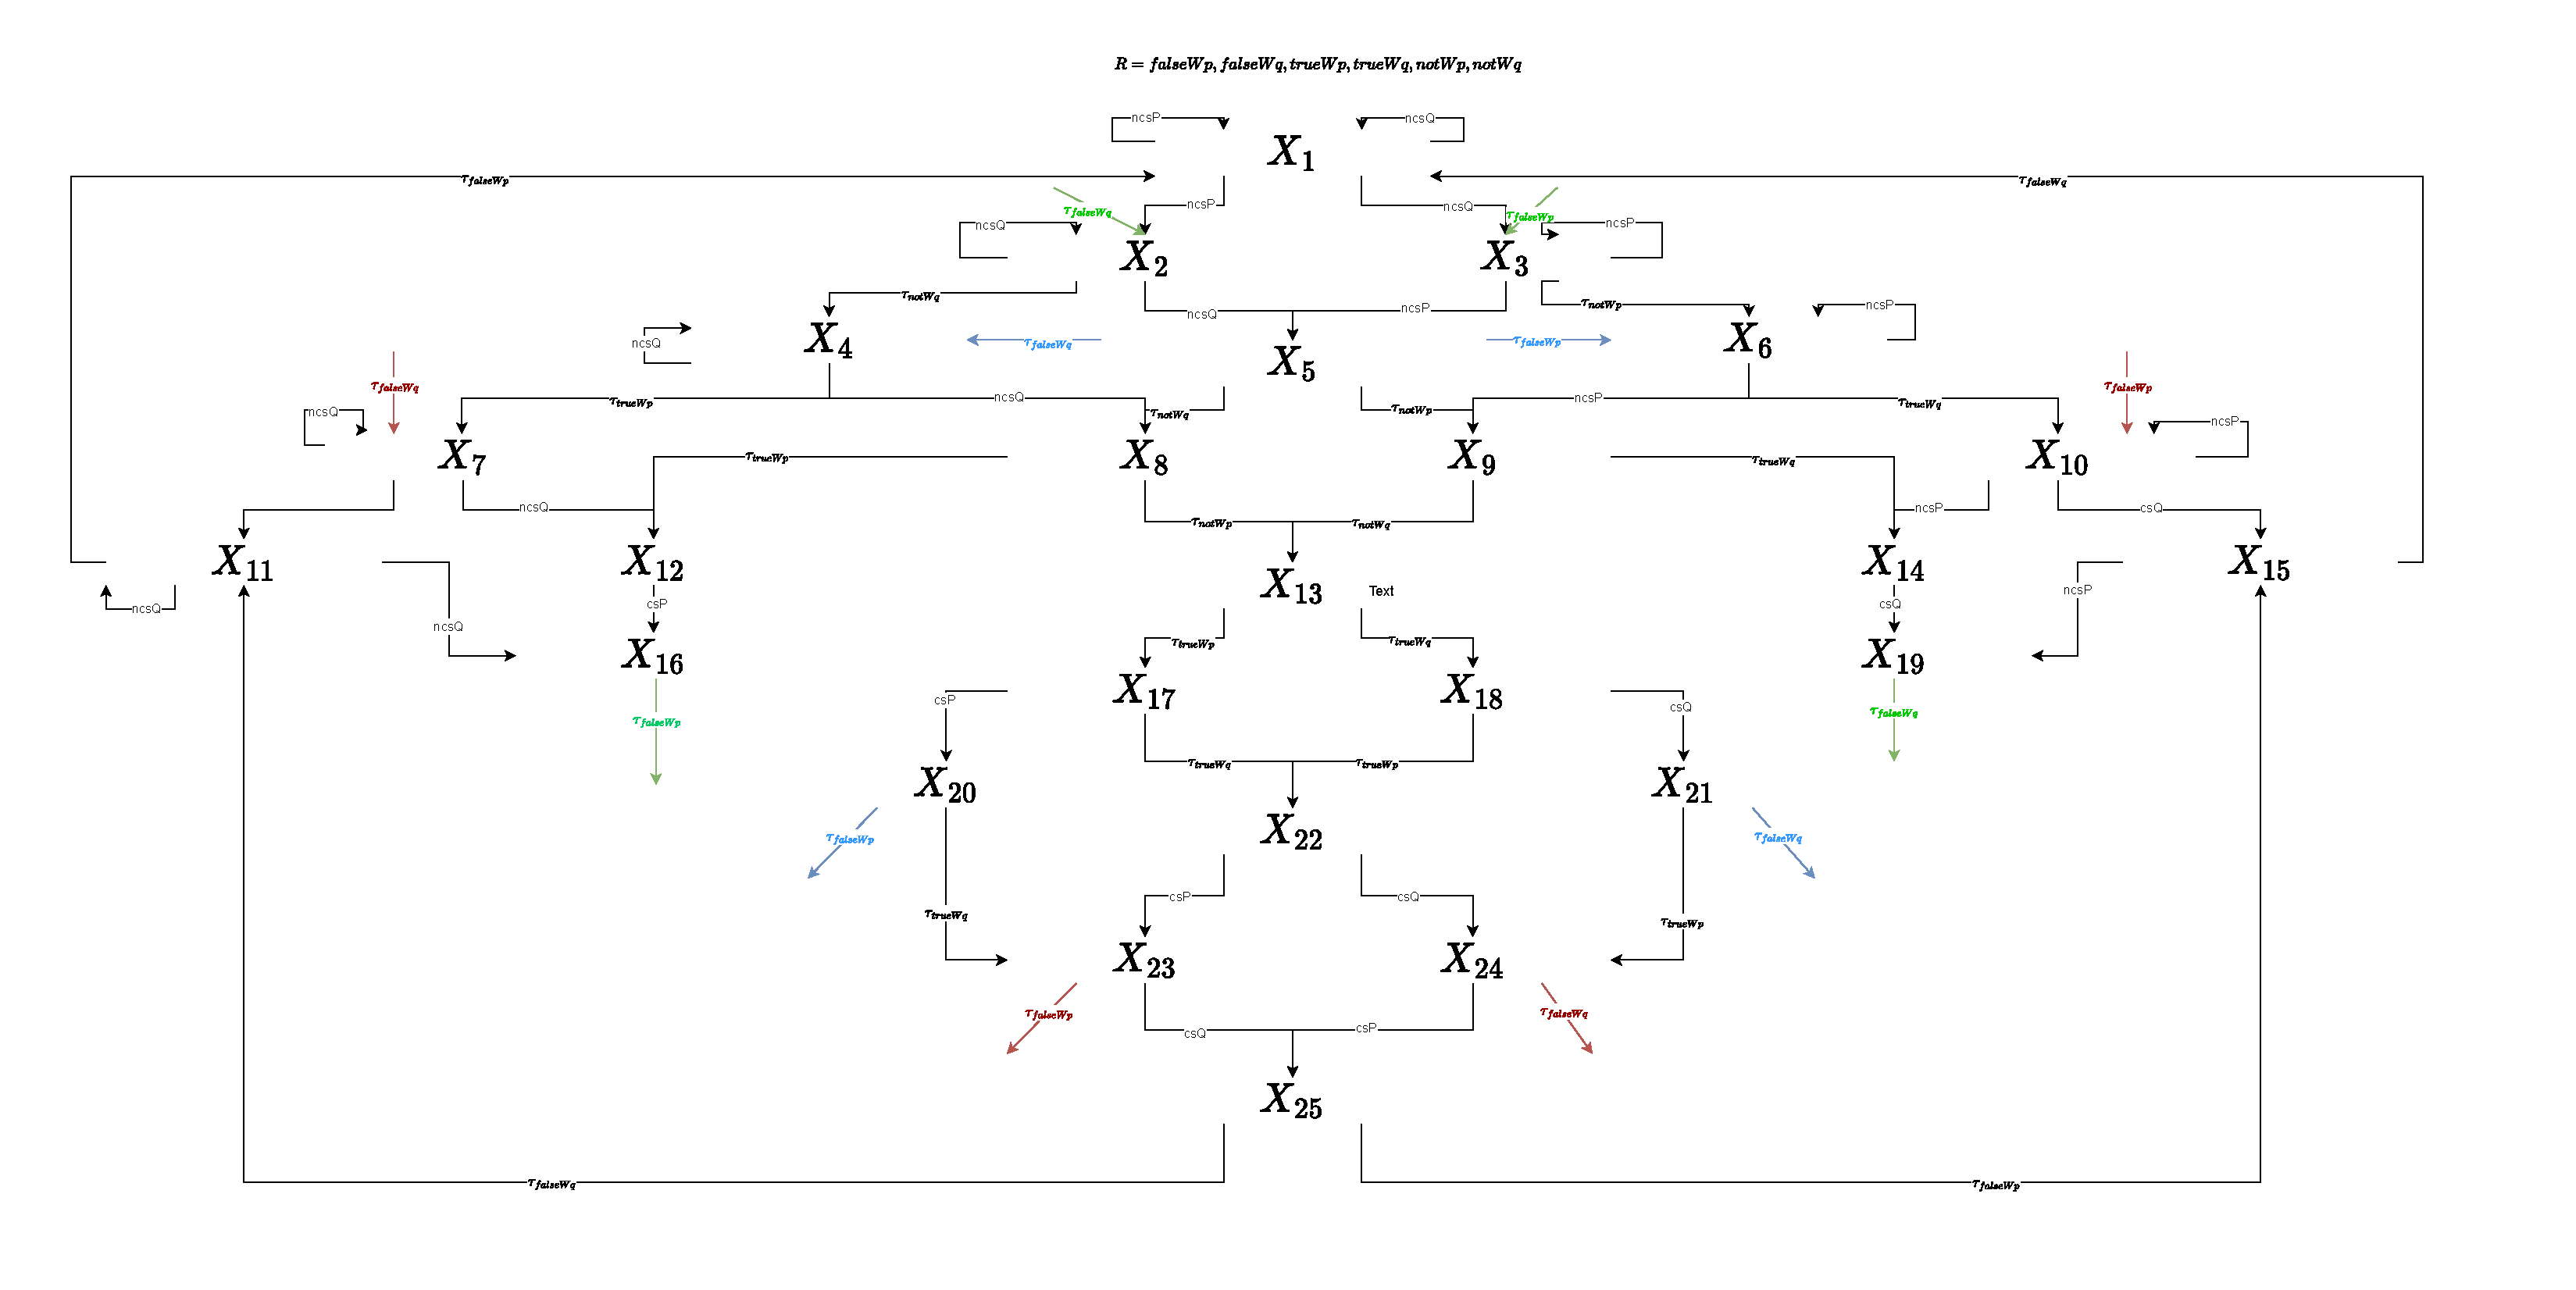
\includegraphics[width=1.6\textwidth]{3_6Eq}}
\caption{Derivation graph 3.6, X} \label{FIG:3.6Eq}
\end{figure*}\\
\newpage
Su questi due \textit{DG} si può eseguire l'algoritmo di bisimulazione.
\begin{align*}
	&A : \{X_1,X_2,X_3,X_4,X_5,X_6,X_7,X_8,X_9,X_{10},X_{11},X_{12},X_{13},X_{14},X_{15},X_{16},X_{17},X_{18},X_{19},
     \\ &X_{20},X_{21},X_{22},X_{23},X_{24},X_{25},Y_1,Y_2,Y_3,Y_4,Y_5,Y_6,Y_7,Y_8,Y_9,Y_{10},Y_{11},Y_{12},Y_{13},Y_{14},Y_{15},Y_{16}\}\\
     \intertext{Divido l'insieme A sull'azione $ncsQ$}
	&A: \{X_1,X_2,X_4,X_7,X_{11},Y_1,Y_2,Y_5,Y_7,Y_9,Y_{11}\}\\
	&B: \{X_3,X_5,X_6,X_8,X_9,X_{10},X_{12},X_{13},X_{14},X_{15},X_{16},X_{17},X_{18},X_{19},\\&X_{20},X_{21},X_{22},X_{23},X_{24},X_{25},Y_3,Y_4,Y_6,Y_8,Y_{10},Y_{12},Y_{13},Y_{14},Y_{15},Y_{16}\}\\
     \intertext{Divido l'insieme B sull'azione $ncsP$ }
	&A: \{X_1,X_2,X_4,X_7,X_{11},Y_1,Y_2,Y_5,Y_7,Y_9,Y_{11}\}\\
	&B: \{X_5,X_8,X_9,X_{12},X_{13},X_{14},X_{16},X_{17},X_{18},X_{19},X_{20},\\& \qquad X_{21},X_{22},X_{23},X_{24},X_{25},Y_4,Y_6,Y_8,Y_{12},Y_{14},Y_{16}\}\\
	&C: \{X_3,X_6,X_{10},X_{15},Y_3,Y_{10},Y_{13},Y_{15} \}\\
     \intertext{Divido l'insieme A sull'azione $\tau$ }
	&A: \{X_1,X_7,Y_1,Y_5,Y_9,Y_{11}\}\\
	&D: \{X_2,X_4,X_{11},Y_2,Y_7\}\\
	&B: \{X_5,X_8,X_9,X_{12},X_{13},X_{14},X_{16},X_{17},X_{18},X_{19},X_{20},\\& \qquad X_{21},X_{22},X_{23},X_{24},X_{25},Y_4,Y_6,Y_8,Y_{12},Y_{14},Y_{16}\}\\
	&C: \{X_3,X_6,X_{10},X_{15},Y_3,Y_{10},Y_{13},Y_{15} \}\\
     \intertext{Divido l'insieme A sull'azione $ncsP$ }
	&A: \{X_1,Y_1,Y_9\}\\
	&E: \{X_7,Y_5,Y_{11}\}\\
	&B: \{X_5,X_8,X_9,X_{12},X_{13},X_{14},X_{16},X_{17},X_{18},X_{19},X_{20},\\& \qquad X_{21},X_{22},X_{23},X_{24},X_{25},Y_4,Y_6,Y_8,Y_{12},Y_{14},Y_{16}\}\\
	&C: \{X_3,X_6,X_{10},X_{15},Y_3,Y_{10},Y_{13},Y_{15} \}\\
	&D: \{X_2,X_4,X_{11},Y_2,Y_7\}\\
     \intertext{Divido l'insieme D sull'azione $ncsP$ }
	&A: \{X_1,Y_1,Y_9\}\\
	&B: \{X_5,X_8,X_9,X_{12},X_{13},X_{14},X_{16},X_{17},X_{18},X_{19},X_{20},\\& \qquad X_{21},X_{22},X_{23},X_{24},X_{25},Y_4,Y_6,Y_8,Y_{12},Y_{14},Y_{16}\}\\
	&C: \{X_3,X_6,X_{10},X_{15},Y_3,Y_{10},Y_{13},Y_{15} \}\\
	&D: \{X_2,X_4\}\\
	&F: \{X_{11},Y_2,Y_7\}\\
	&E: \{X_7,Y_5,Y_{11}\}\\
     \intertext{Divido l'insieme A sull'azione $ncsP$ }
	&A: \{X_1,Y_9\}\\
	&G: \{Y_1\}\\
	&B: \{X_5,X_8,X_9,X_{12},X_{13},X_{14},X_{16},X_{17},X_{18},X_{19},X_{20},\\& \qquad X_{21},X_{22},X_{23},X_{24},X_{25},Y_4,Y_6,Y_8,Y_{12},Y_{14},Y_{16}\}\\
	&C: \{X_3,X_6,X_{10},X_{15},Y_3,Y_{10},Y_{13},Y_{15} \}\\
	&D: \{X_2,X_4\}\\
	&E: \{X_7,Y_5,Y_{11}\}\\
	&F: \{X_{11},Y_2,Y_7\}\\
\end{align*}
Dato che $X_1$ e $Y_1$ si trovano rispettivamente in $A$ e $E$ quindi non sono in relazione di bisimulazione tra loro.
\newpage
\section{Algoritmo 3.8}
\label{SEC:3.8}
\begin{center}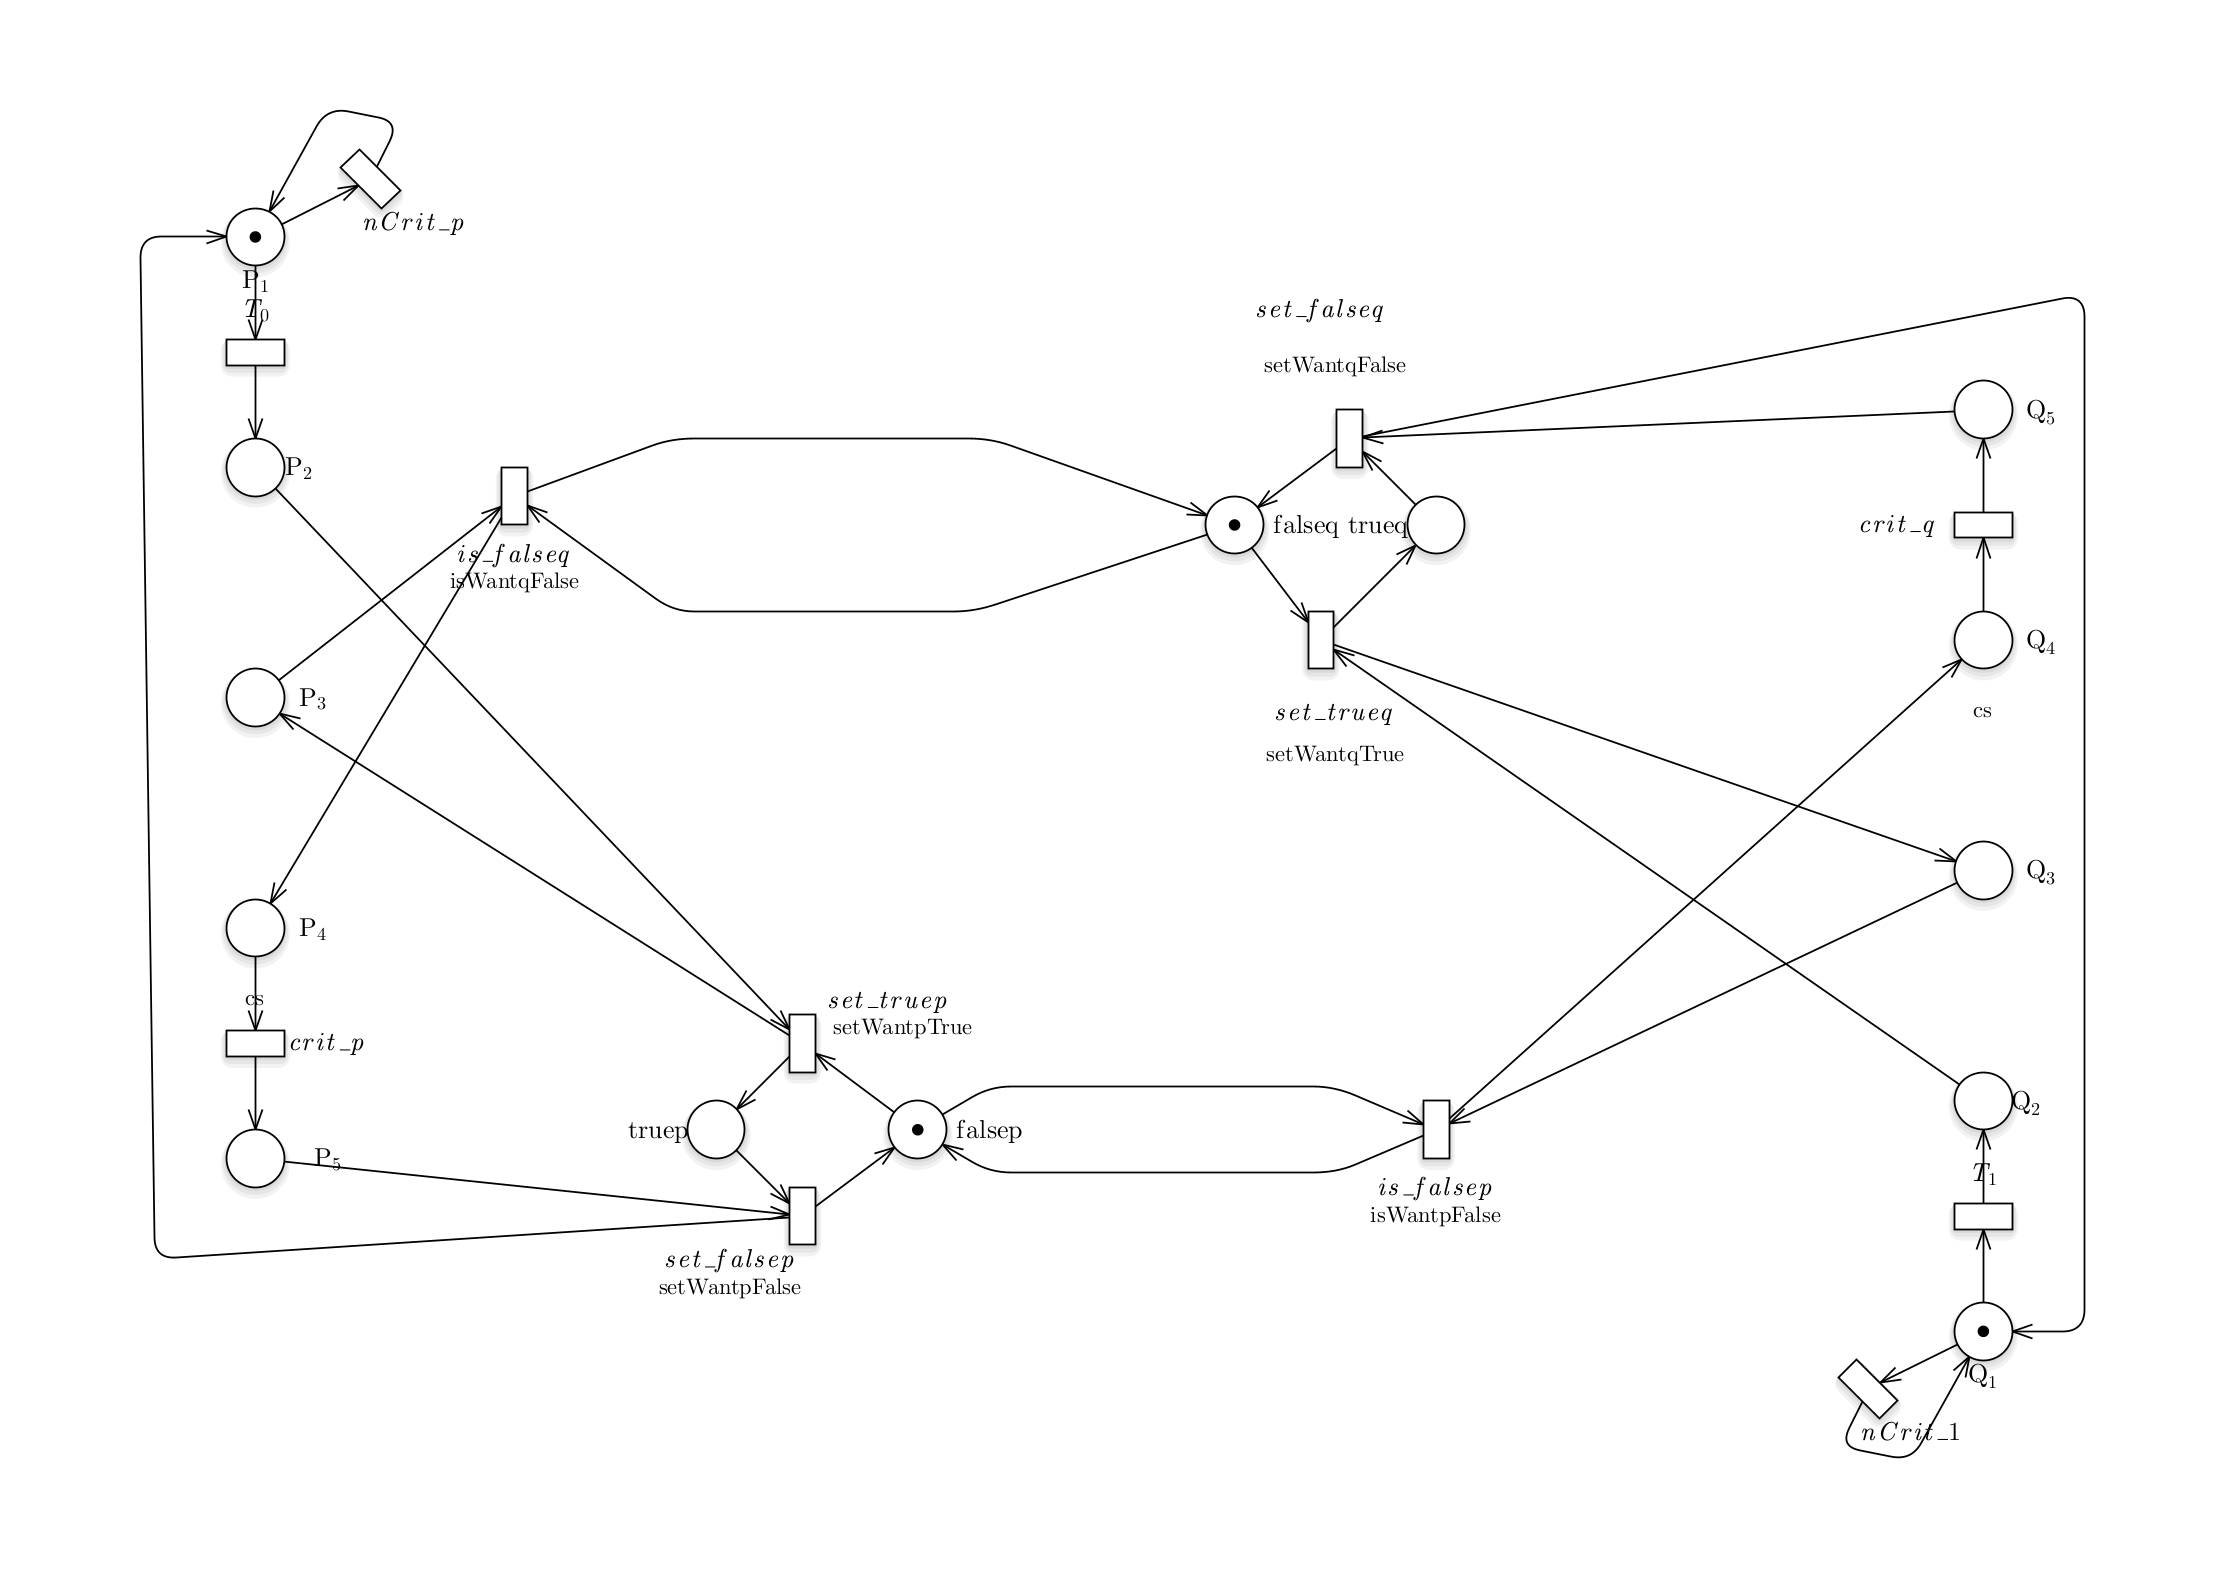
\includegraphics[width=1\textwidth]{3.8.png}\end{center}
Questo algoritmo cerca di risolvere il problema del 3.6 (sezione \ref{SEC:3.6}) andando ad invertire l'operazione di setting della variabile che si riferisce al voler entrare in sezione critica e l'operazione di attesa sulla variabile che indica l'intenzione dell'altro processo
\subsection{Rete di Petri}
In questo caso è stata anche effettuata una modifica alle variabili rimuovendo le transizioni \texttt{is\_true}, in quanto nell'algoritmo 3.8 non viene mai controllato se una variabile è vera.
\newpage
\begin{center}
\makebox[\textwidth][c]{
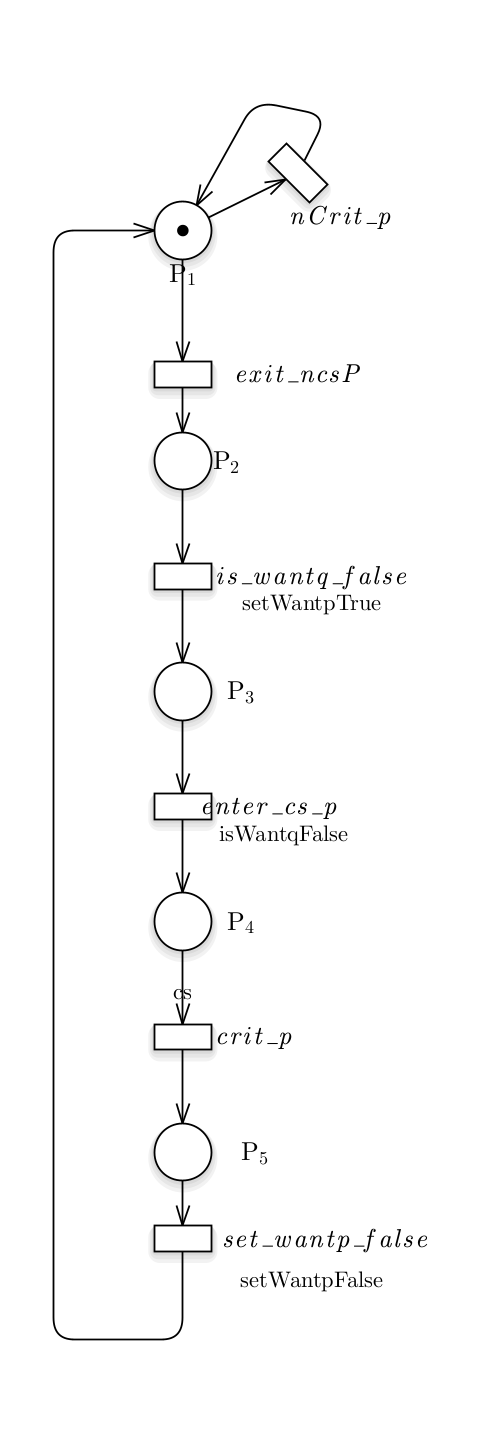
\includegraphics[width=0.4\textwidth]{p3.8.png}
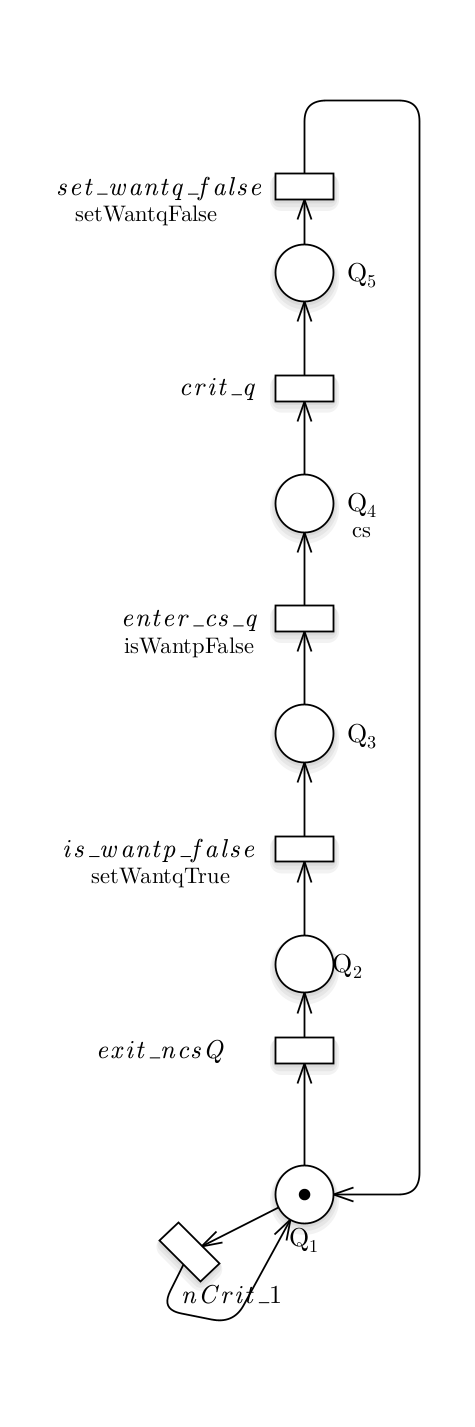
\includegraphics[width=0.4\textwidth]{q3.8.png}
}
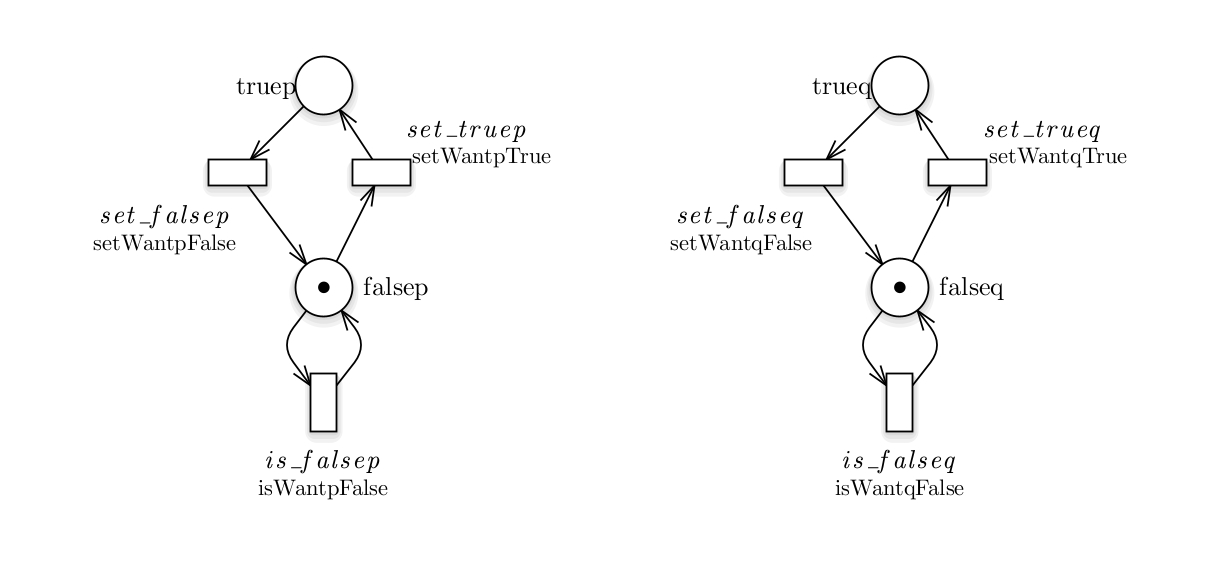
\includegraphics[width=0.8\textwidth]{variables_noTrue.png}
\end{center}
\newpage
\begin{figure*}[!ht]
\centering
\makebox[\textwidth][c]{
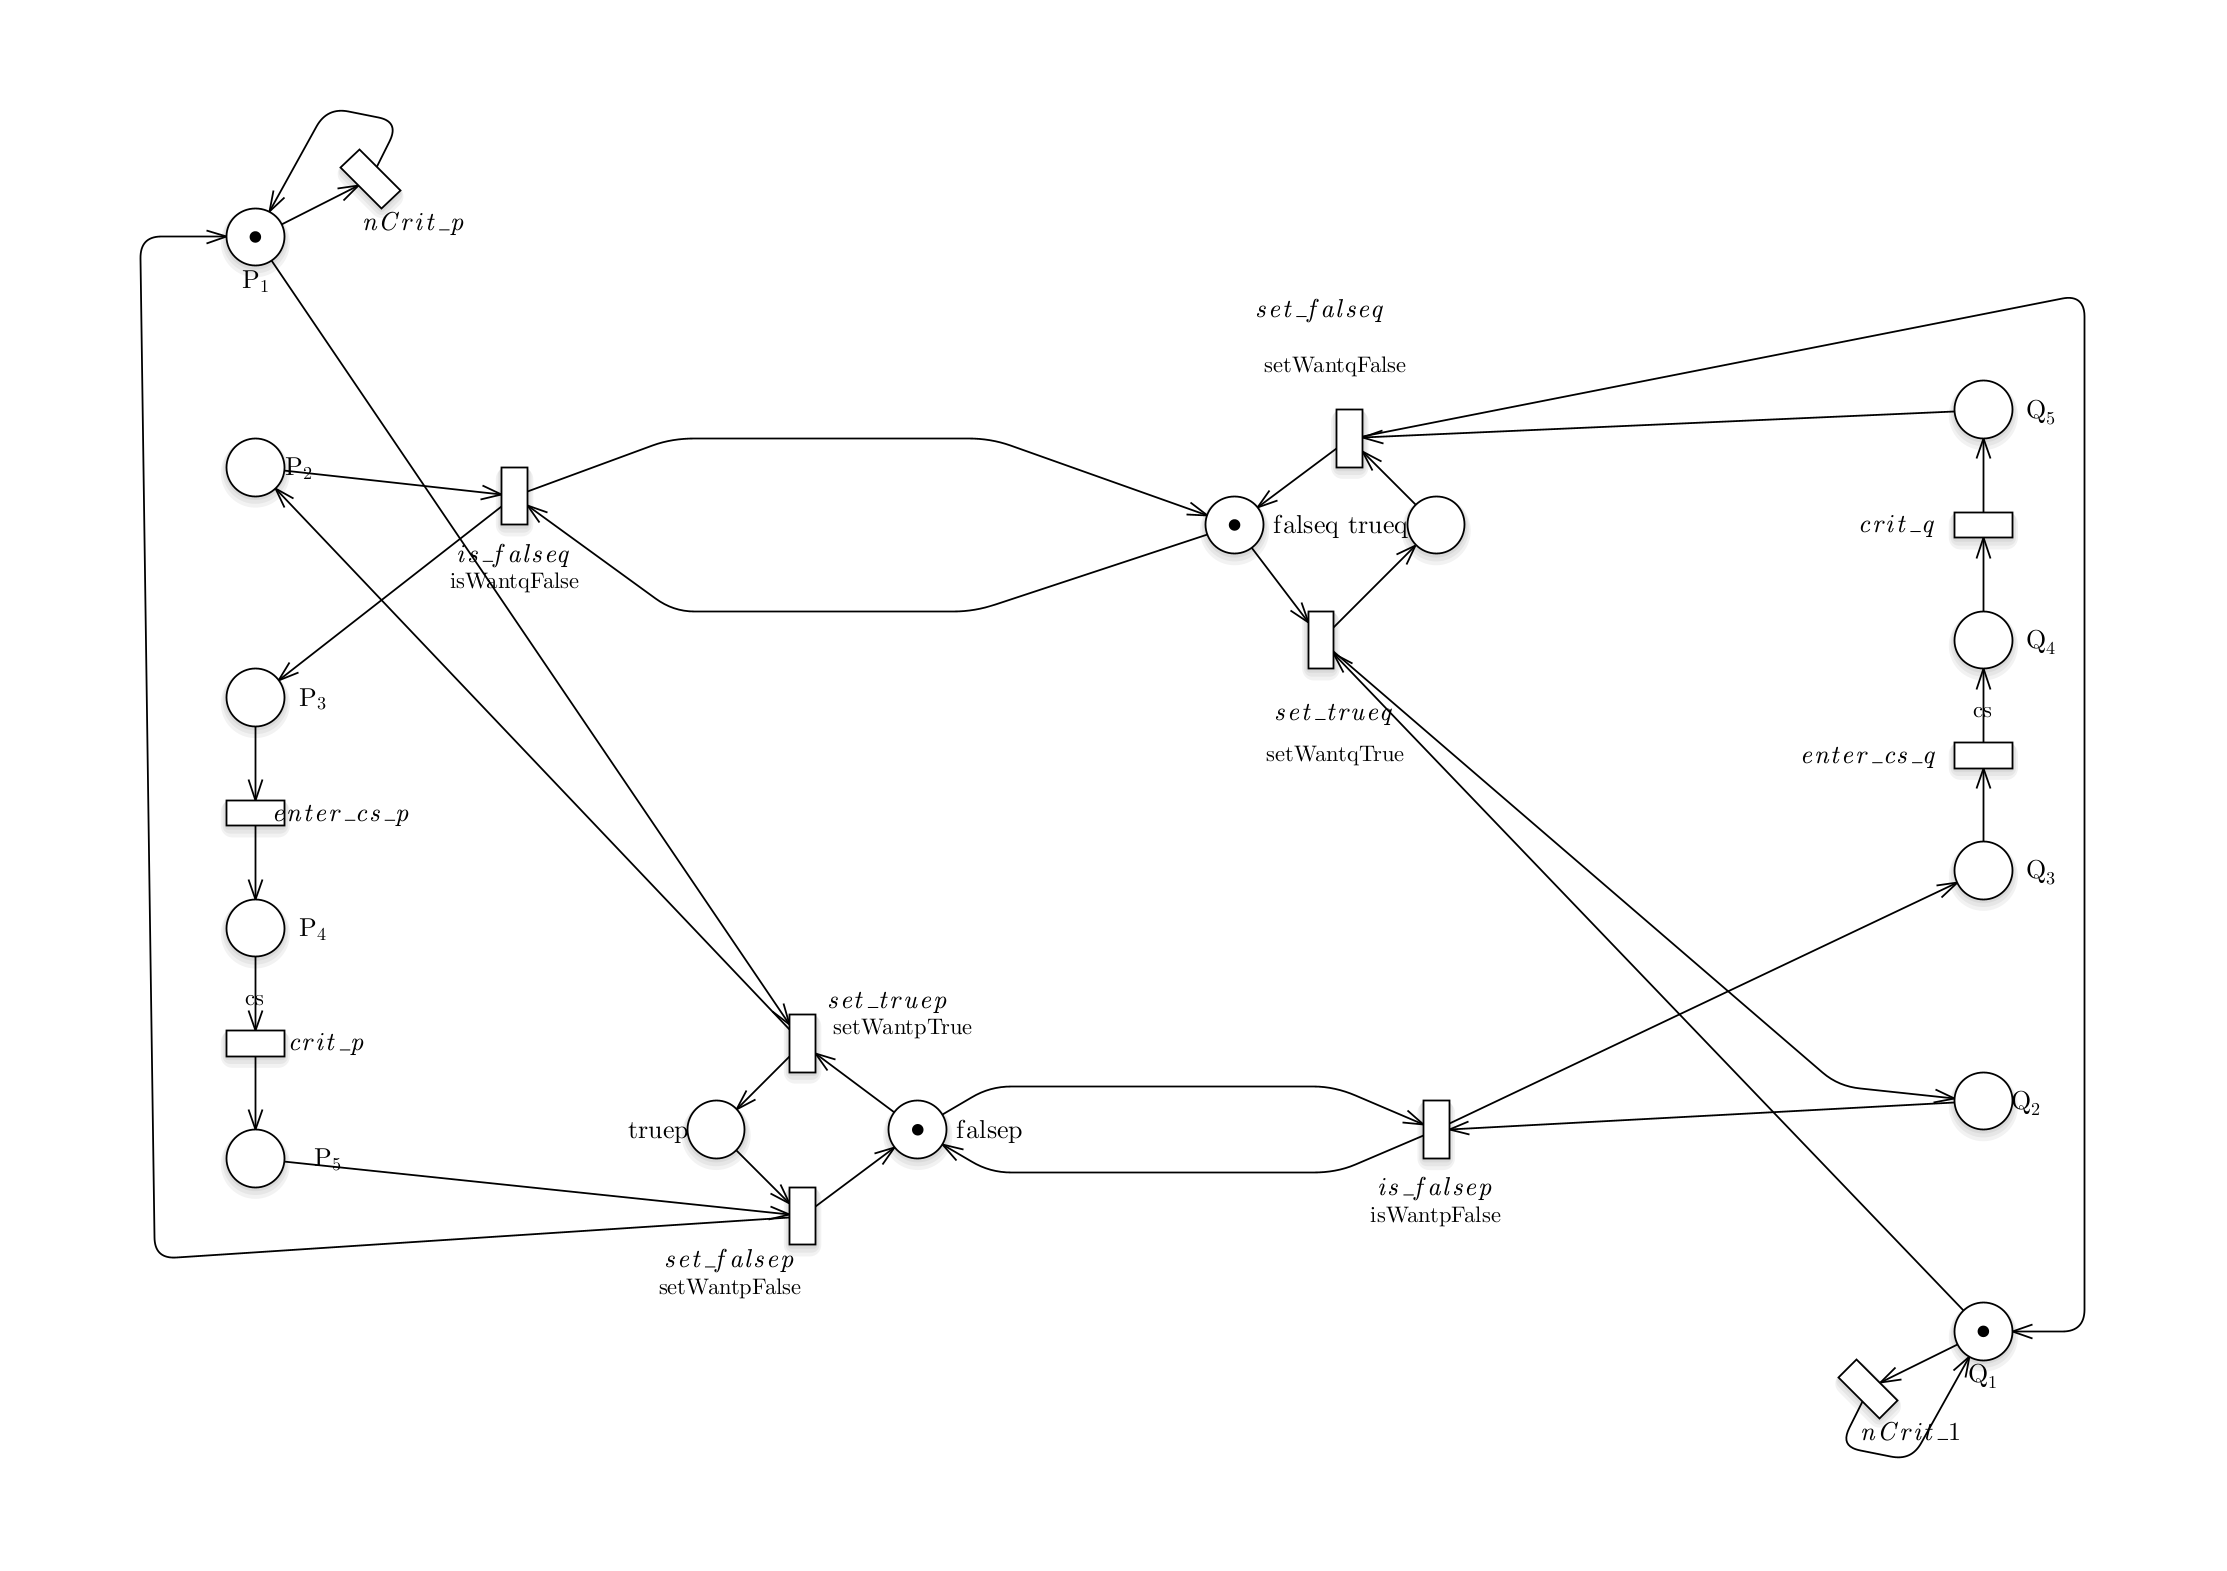
\includegraphics[width=1.6\textwidth]{3.8PN.png}}
\caption{Rete di petri composta} \label{FIG:3.8PN}
\end{figure*}
\newpage
\subsubsection{RG}
Il reachability graph, in figura \ref{FIG:3.8RG}, è composto 21 stati, di cui uno rappresentante una situazione di Deadlock.
\begin{figure*}[!ht]
\centering
\makebox[\textwidth][c]{
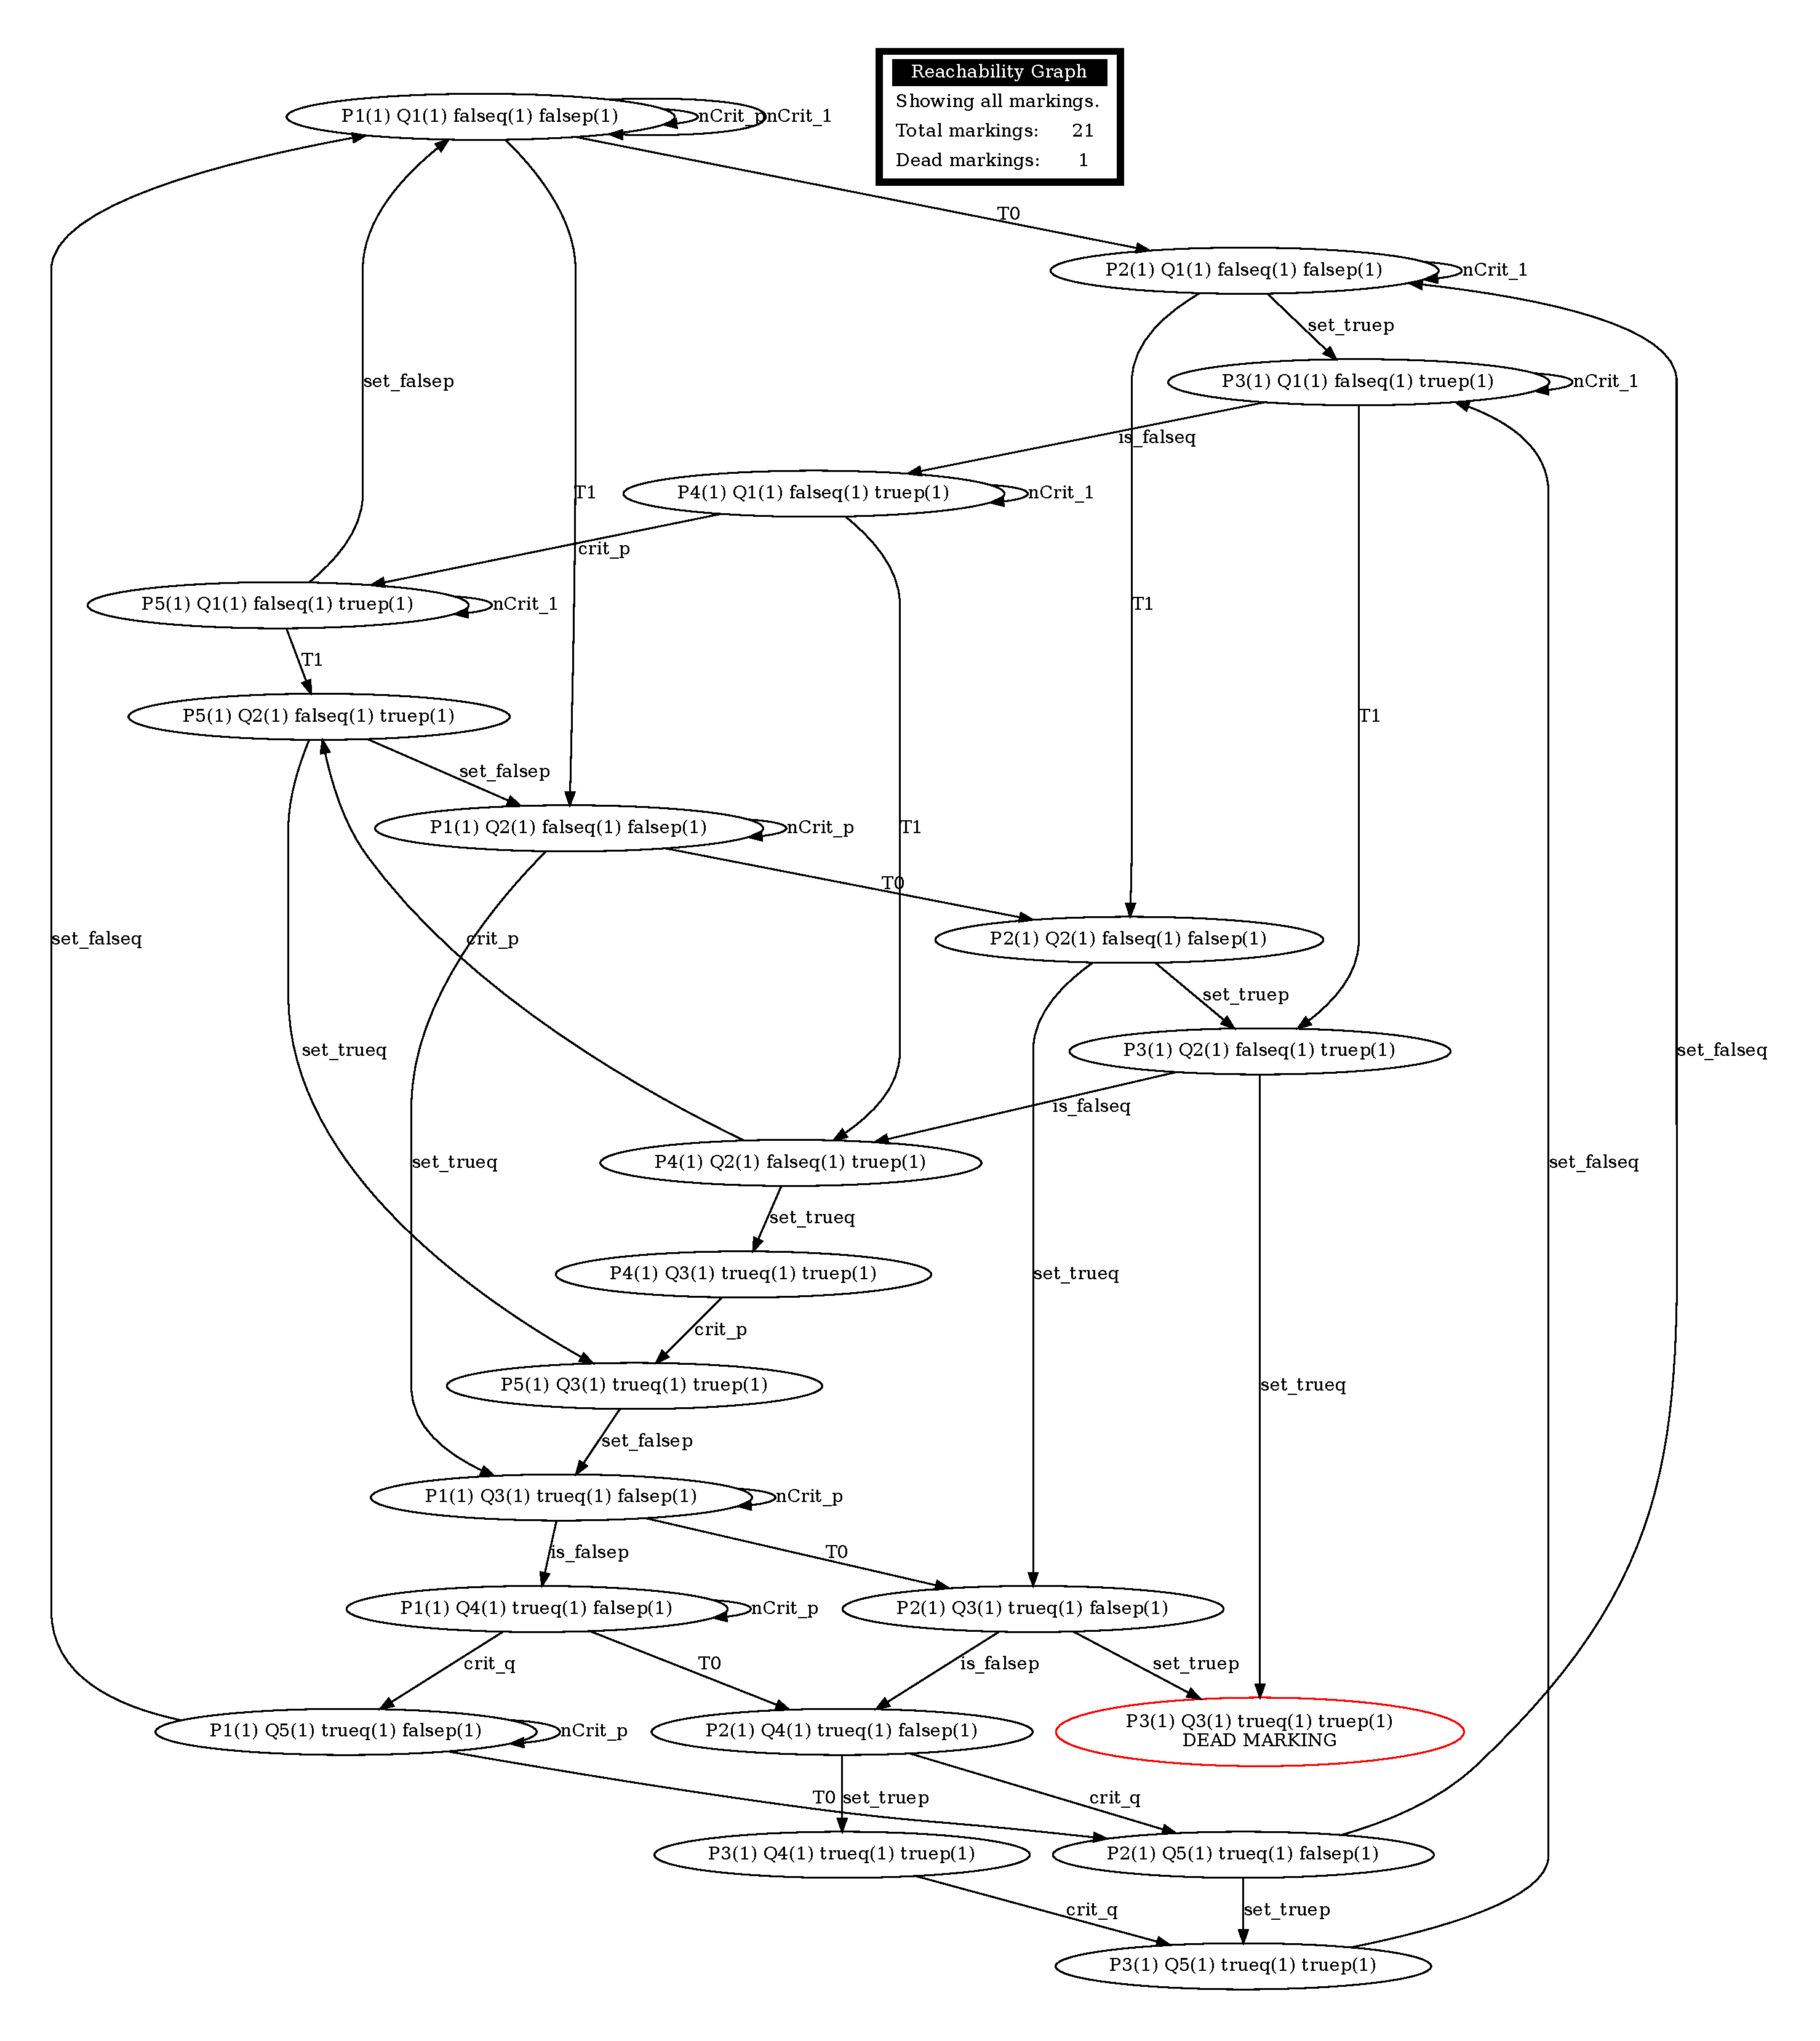
\includegraphics[width=1\textwidth]{3.8RG}}
\caption{Reachability graph 3.8} \label{FIG:3.8RG}
\end{figure*}
\newpage
\subsubsection{Analisi strutturale}
Il calcolo dei \textit{semiflow} è sostanzialmente identico a quello effettuato in sezione \ref{SEC:3_8_strutturale} in quanto la struttura della rete non è cambiata molto.
Lo studio dei \textit{P-invarianti} rivela che tutti i posti sono 1-bound, che le variabili assumono un solo valore di verità alla volta e che i token che rappresentano il program counter si trovano in un solo posto alla volta per ogni processo.
Anche lo studio dei \textit{T-semiflow} è pressochè identico.
Nonostante il sistema abbia uno stato di deadlock una \textit{firing sequence} che riporta il sistema nella marcatura iniziale esiste, quindi il sistema possiede la proprietà di \textit{liveness}.\\

\subsubsection{Model Checking GreatSPN}
Sono state verificate le seguenti formule CTL:
\begin{itemize}
	\item mutua esclusione: \textit{AG !(\#P4==1 \&\& \#Q4==1)} \textcolor{green}{true}.\\
		Il sistema rispetta la mutua esclusione.
	\item deadlock: \textit{AG AF ((\#P1==1) || (\#Q1 == 1))} \textcolor{red}{false}.\\
		Il sistema va in deadlock, il controesempio presentato dal Model Checker è l'esecuzione $\{P_1Q_1 \rightarrow P_1Q_2 \rightarrow P_2Q_2\}$.
	\item assenza di starvation: \textit{AG((\#P2 >0 ) -> (AF i\#P4>0 ))} ed anche \textit{AG((\#P2 >0 ) -> (AF i\#P4>0 ))}. Entrambe risultano \textcolor{red}{false}.\\
		Essendoci deadlock c'è sempre la possibilità di starvation. Se il sistema va in deadlock dopo l'esecuzione presentata nel punto precedente entrambi i processi presentano starvation.
\end{itemize}
Sono state verificate le seguenti formule LTL:
\begin{itemize}
	\item mutua esclusione: \textit{G !(\#P4==1 \&\& \#Q4==1)} \textcolor{green}{true}.
	\item assenza di starvation: \textit{G F (\#P2==1) -> G F(\#P4 == 1)} ed anche \textit{G F (\#Q2==1) -> G F(\#Q4 == 1)}. Entrambe risultano \textcolor{red}{false}.
	\item deadlock: \textit{G F( (\#P1 ==1) ||  (\#Q1 ==1))} \textcolor{red}{false}.
\end{itemize}
\newpage
\subsection{NuSMV}
L'implementazione del sistema tramite il linguaggio di NuSMV è pressochè identica a quella della sezione \ref{SUBSEC:3.6NuSMV}, l'unica differenza sta nella posizione del controllo \texttt{!want\_other} che questa volta viene effettuato dopo aver impostato la variabile \textit{want\_me} a true.
\lstinputlisting{figures/3_8_code.smv}
Il comando \texttt{print\_reachable\_states} mostra 21 stati raggiungibili di 100 possibili, in linea con la dimensione del Reachability Graph.
È presente uno stato di deadlock : $p.state=s3, \; q.state=s3, \; wantp = true, \; wantq = true $. 

\subsubsection{Model Checking NuSMV}
Sono state verificate le seguenti formule CTL:
\begin{itemize}
        \item mutua esclusione: \textit{AG !(( p.state = s4 ) \& (q.state = s4 ))} \textcolor{green}{true}.
        \item deadlock: \textit{AG AF (( p.state = s1 )| ( q.state = s1 ))} \textcolor{red}{false}.\\
		Il sistema va in deadlock, il controesempio presentato dal Model Checker è una esecuzione che fa eseguire tutti gli stati di q tornando a q.state= s1 e poi esegue $\{P_1Q_1 \rightarrow P_1Q_2 \rightarrow P_2Q_2\}$ che lo porta in deadlock.
        \item assenza di starvation: \textit{AG (( p.state = s2 ) -> (AF p.state = s3 ))} ed anche \textit{AG (( q.state = s2 ) -> (AF q.state = s3 ))}. Entrambe risultano \textcolor{red}{false}.\\
		Essendoci deadlock c'è sempre la possibilità di starvation. Se il sistema va in deadlock dopo l'esecuzione presentata precedente entrambi i processi presentano starvation.
		L'esempio presentato dal Model Checker è lo stesso del caso di deadlock.
\end{itemize}
Sono state verificate le seguenti formule LTL:
\begin{itemize}
        \item mutua esclusione: \textit{G !(p.state = s4 \& q.state = s4)} \textcolor{green}{true}.
        \item deadlock: \textit{G F(( p.running) | ( q.running ) )} \textcolor{red}{false}. \\
		Il sistema va in deadlock, il controesempio presentato dal Model Checker è una esecuzione che fa eseguire tutti gli stati di q tornando a q.state= s1 e poi esegue $\{P_1Q_1 \rightarrow P_1Q_2 \rightarrow P_2Q_2\}$ che lo porta in deadlock.
        \item assenza di starvation: \textit{G (p.state = s2 ->  F p.state = s3)} ed anche \textit{G (p.state = s2 ->  F p.state = s3)}. Entrambe risultano \textcolor{red}{false}.\\
		Essendoci deadlock c'è sempre la possibilità di starvation. Se il sistema va in deadlock dopo l'esecuzione presentata precedente entrambi i processi presentano starvation.
		L'esempio presentato dal Model Checker è lo stesso del caso di deadlock in CTL.
\end{itemize}

\section{Confronto e riduzione di 3.6 e 3.8}

\subsection{Riduzione Algoritmo 3.6}
Per prima cosa con l'operazione \textit{RC2} è possibile eliminare i due self-loop \textit{nCrit\_p \textit{e} nCrit\_q}.
I posti $P_4,P_5$ e $Q_4,Q_5$ possono essere ridotti tramite \textit{RA1}.
Le transizioni $access\_crit\_p$ e $access\_crit\_q$ possono essere rimosse tramite l'utilizzo di \textit{RA1}.
Si può infine unire $is\_falseq$ con $set\_truep$ e $is\_falsep$ con $set\_trueq$ grazie a \textit{RA2}.
La rete risultate è visibile in figura \ref{FIG:3.6Red}
\begin{figure*}[!ht]
\centering
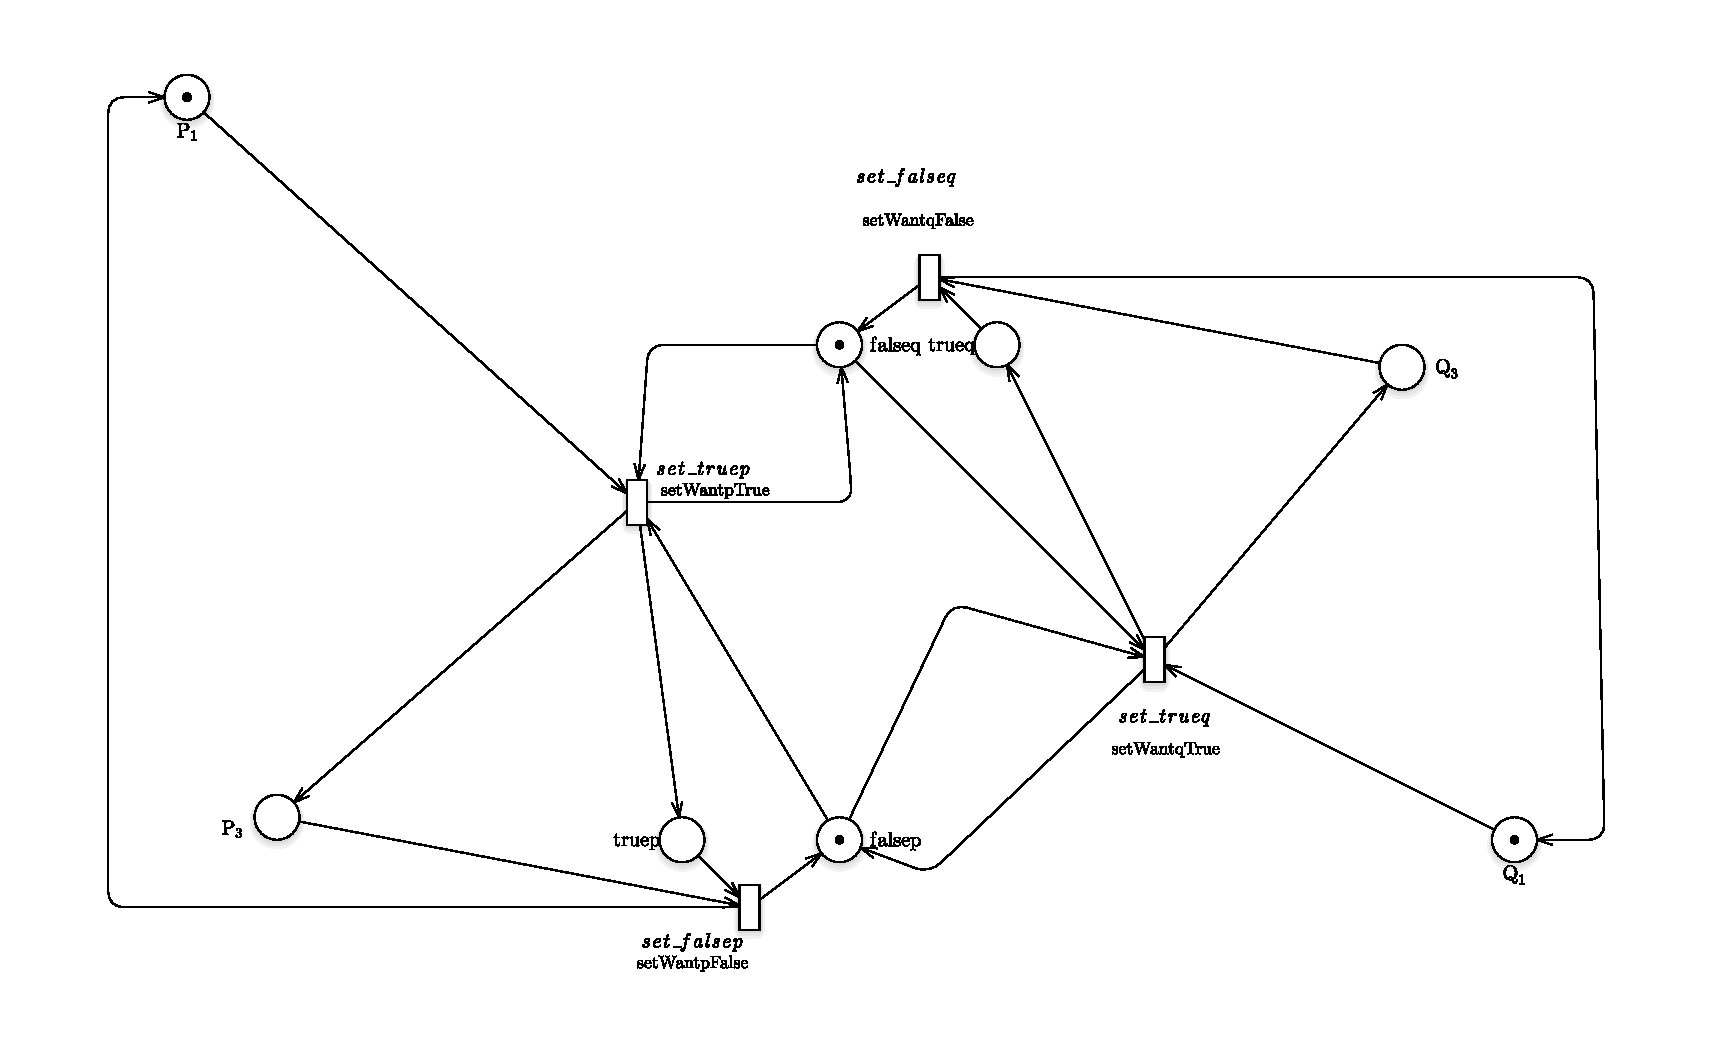
\includegraphics[width=1\textwidth]{3.6Red}
\caption{Rete algoritmo 3.6 ridotta} \label{FIG:3.6Red}
\end{figure*}

\subsection{Riduzione Algoritmo 3.8}
Per prima cosa con l'operazione \textit{RC2} è possibile eliminare i due self-loop \textit{nCrit\_p \textit{e} nCrit\_q}.
Le transizioni $access\_crit\_p$ e $access\_crit\_q$ possono essere rimosse tramite l'utilizzo di \textit{RA1}, unendo i posti $P_1,P_2$ e $Q_1, Q_2$.
I posti $P_4,P_5$ e $Q_4,Q_5$ possono essere ridotti tramite \textit{RA1}.
La rete risultate è visibile in figura \ref{FIG:3.8Red}
\begin{figure*}[!ht]
\centering
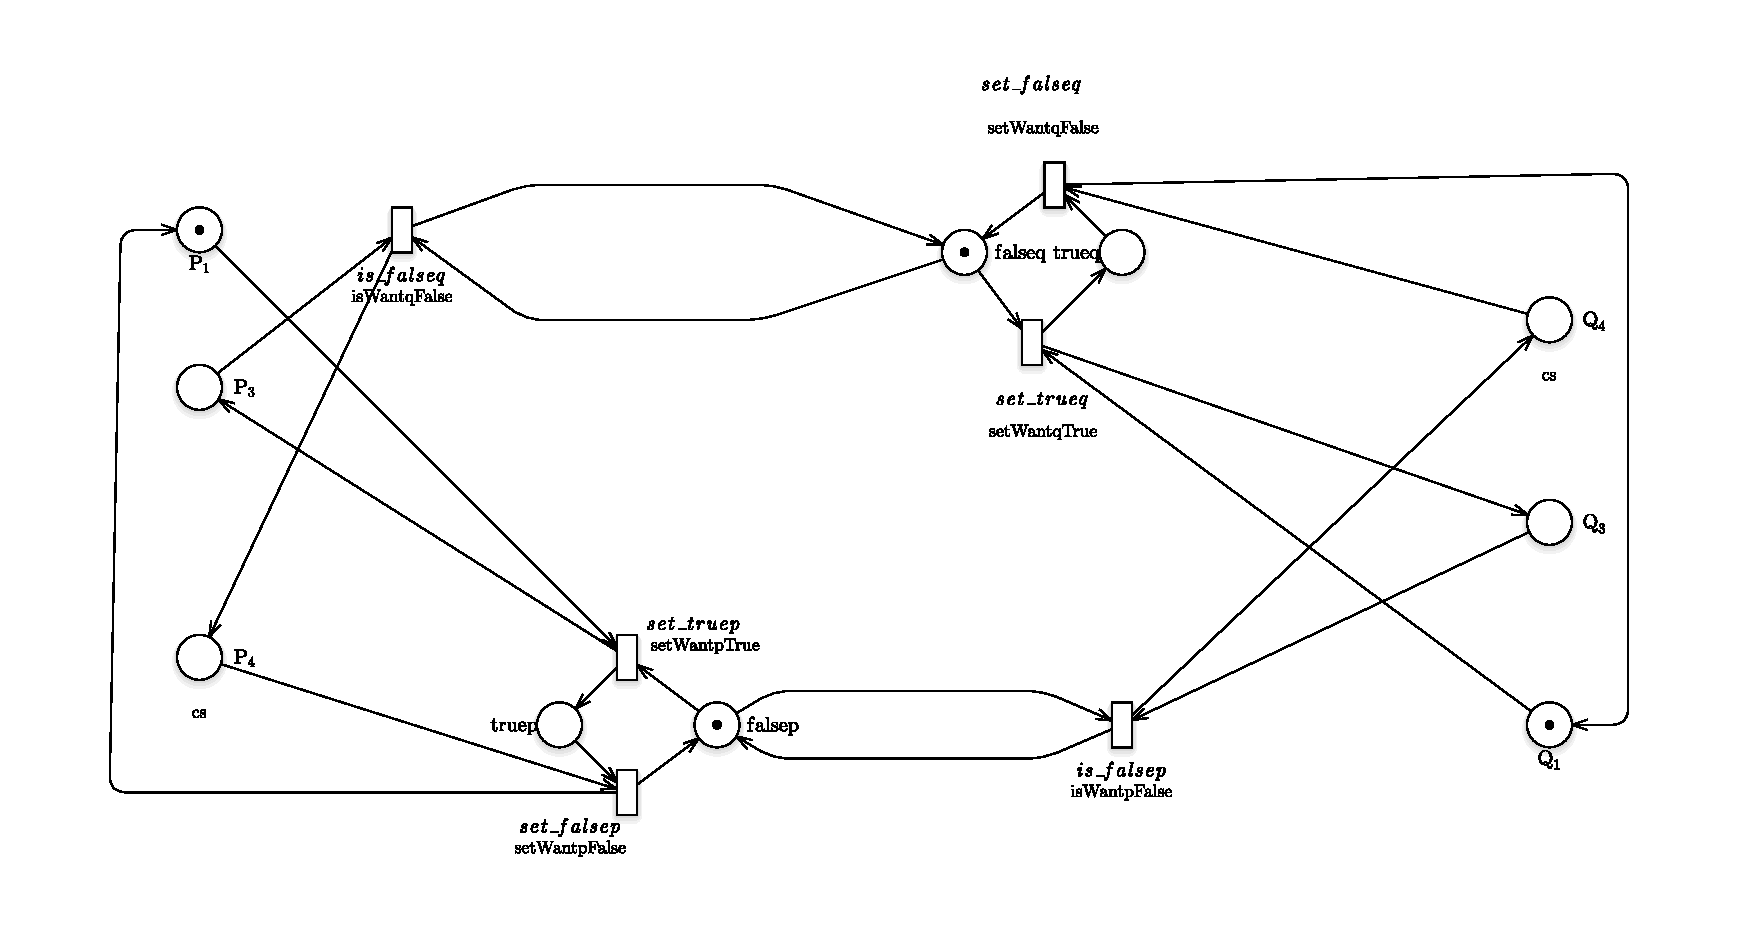
\includegraphics[width=1\textwidth]{3.8Red}
\caption{Rete algoritmo 3.8 ridotta} \label{FIG:3.8Red}
\end{figure*}

\subsection{Confronto}
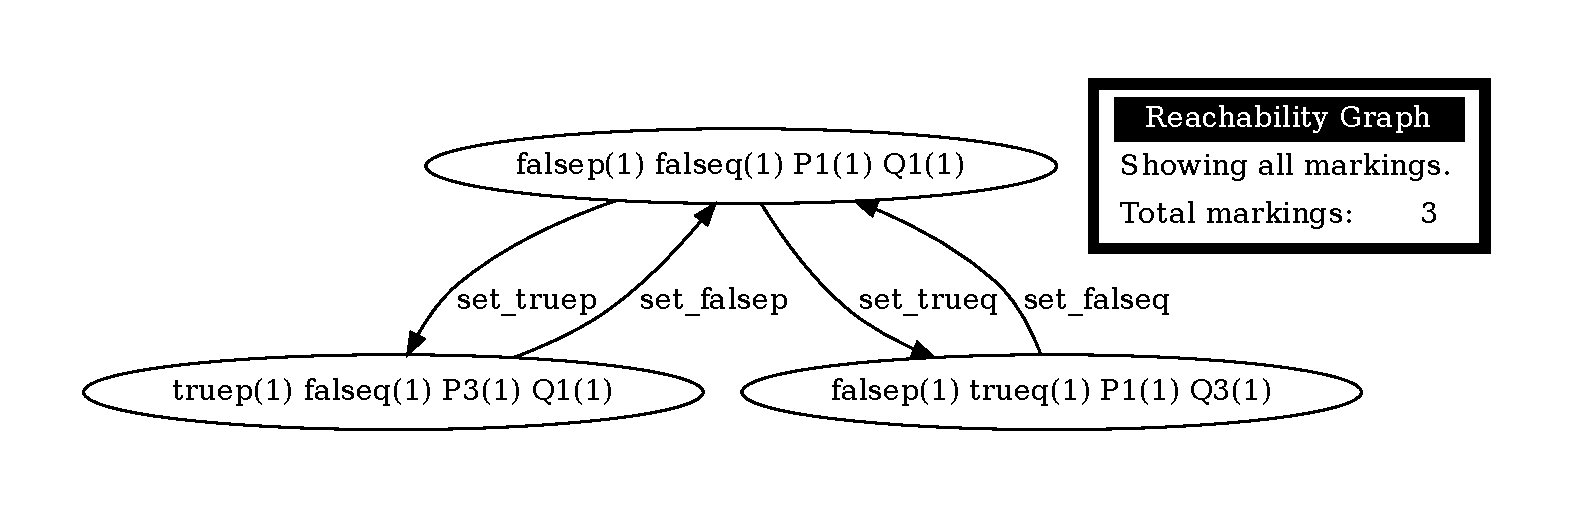
\includegraphics[width=1\textwidth]{3.6RedRG}
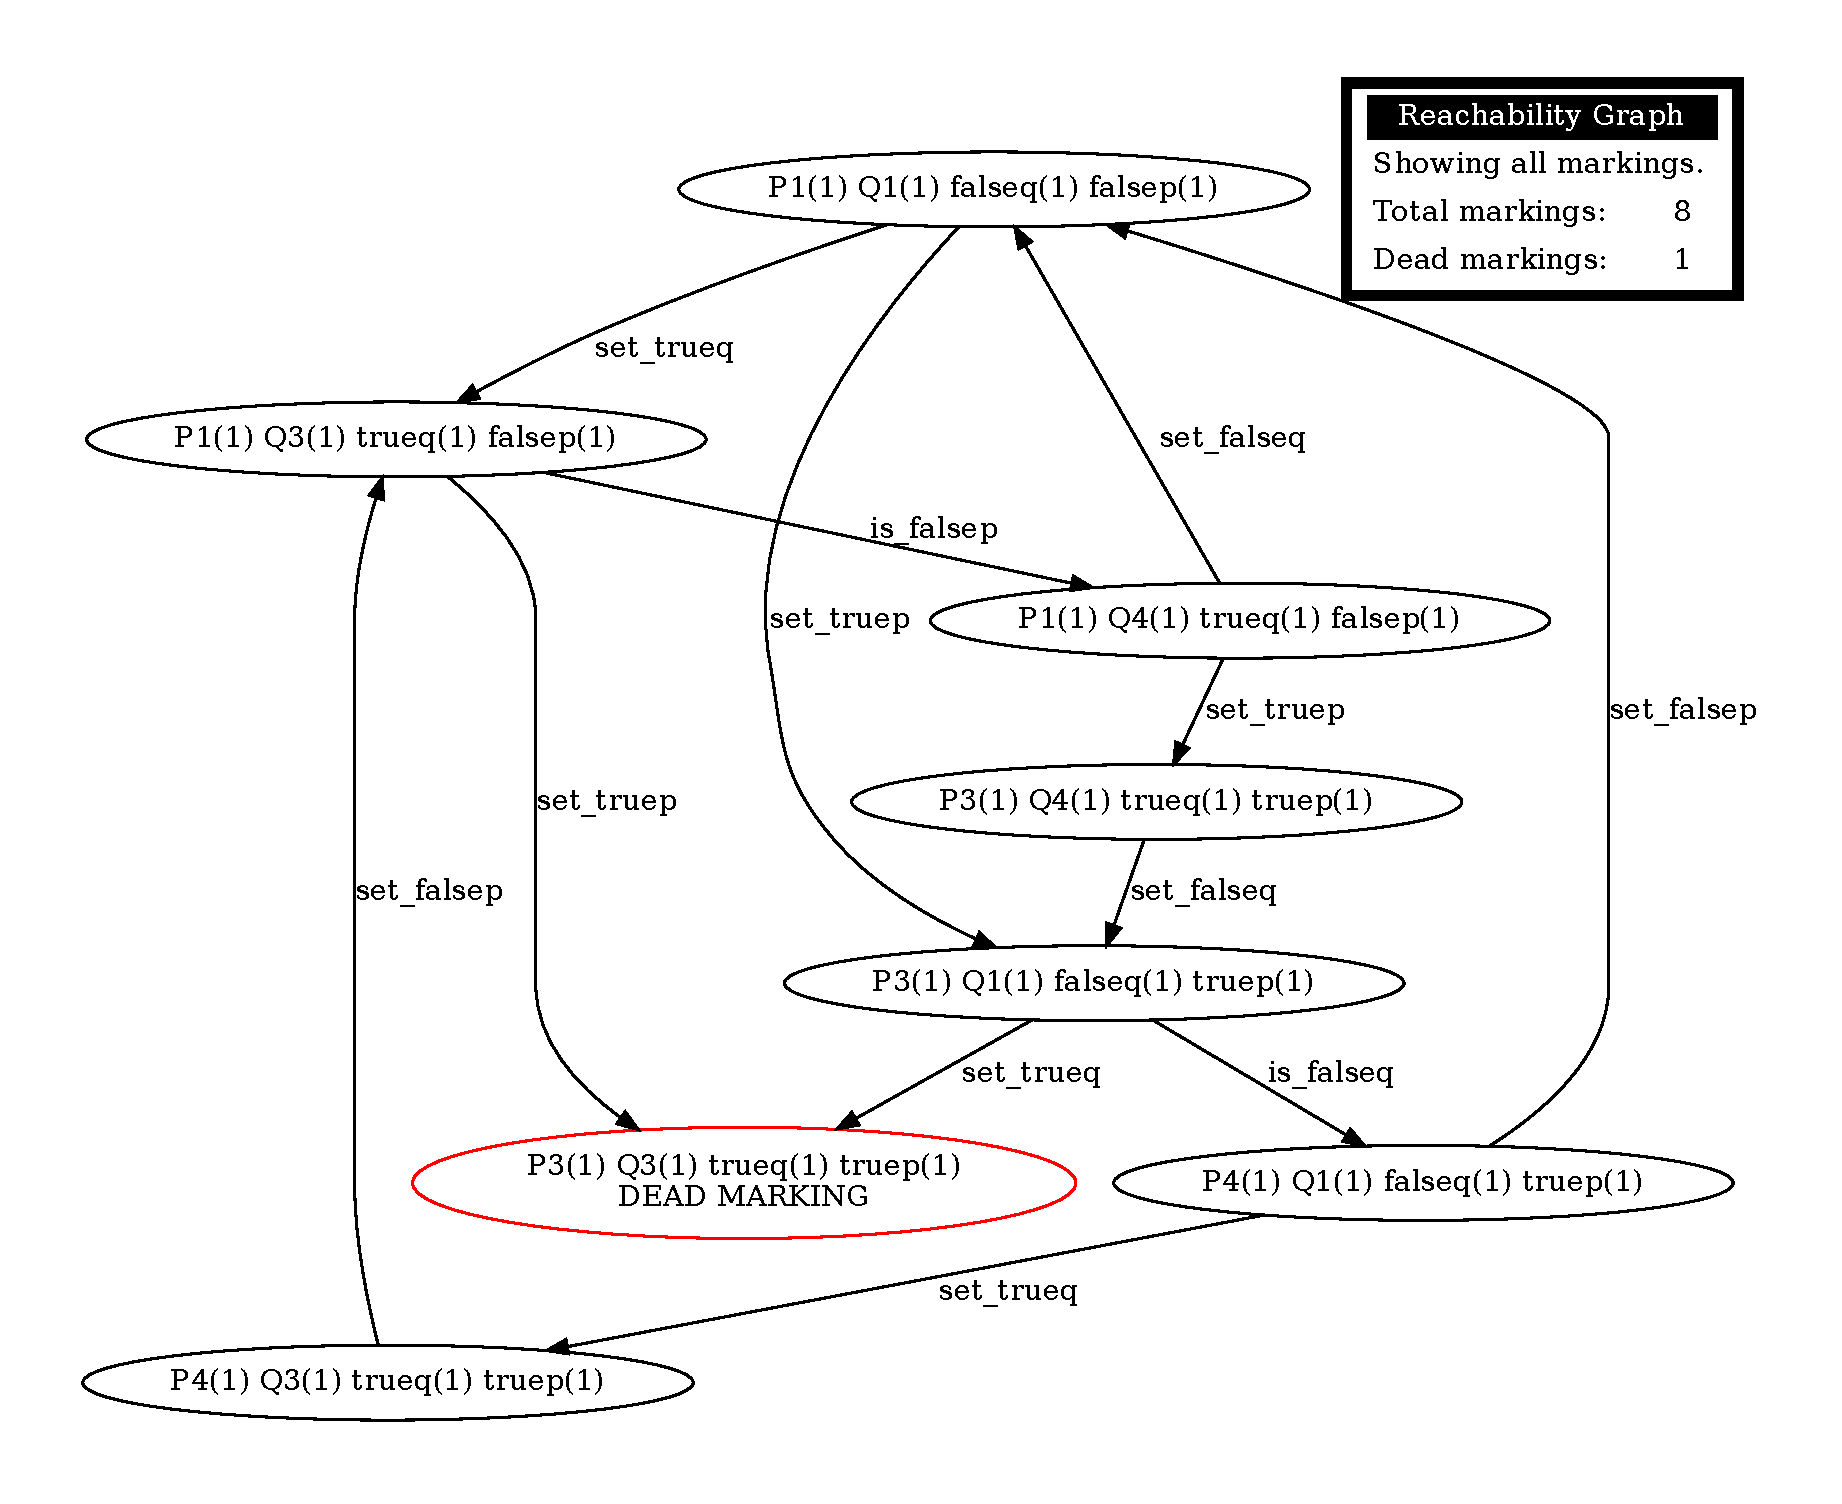
\includegraphics[width=1\textwidth]{3.8RedRG}
%TODO: la non equivalenza alle tracce basta ad affermare che non sono bisimili?
I due sistemi non sono equivalenti alle tracce, come prova si può prendere la sequenza $[set\_truep,set\_trueq]$ che può essere eseguita solo dall'algoritmo 3.8 e non dal 3.6.
Non essendo equivalenti alle tracce sicuramente non sono equivalenti ai fallimenti, alla simulazione ed alla bisimulazione.

\newpage
\section{Algoritmo 3.9}
\label{SEC:3.9}
\begin{center}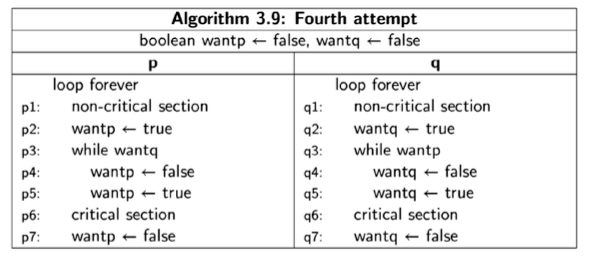
\includegraphics[width=1\textwidth]{3.9.png}\end{center}
Questo algoritmo cerca di risolvere il deadlock del 3.8 \ref{SEC:3.6} andando a resettare il valore della variabile che si riferisce al voler entrare in sezione critica qualora non si riesca ad entrare.
\subsection{Rete di Petri}
\newpage
\begin{center}
\makebox[\textwidth][c]{
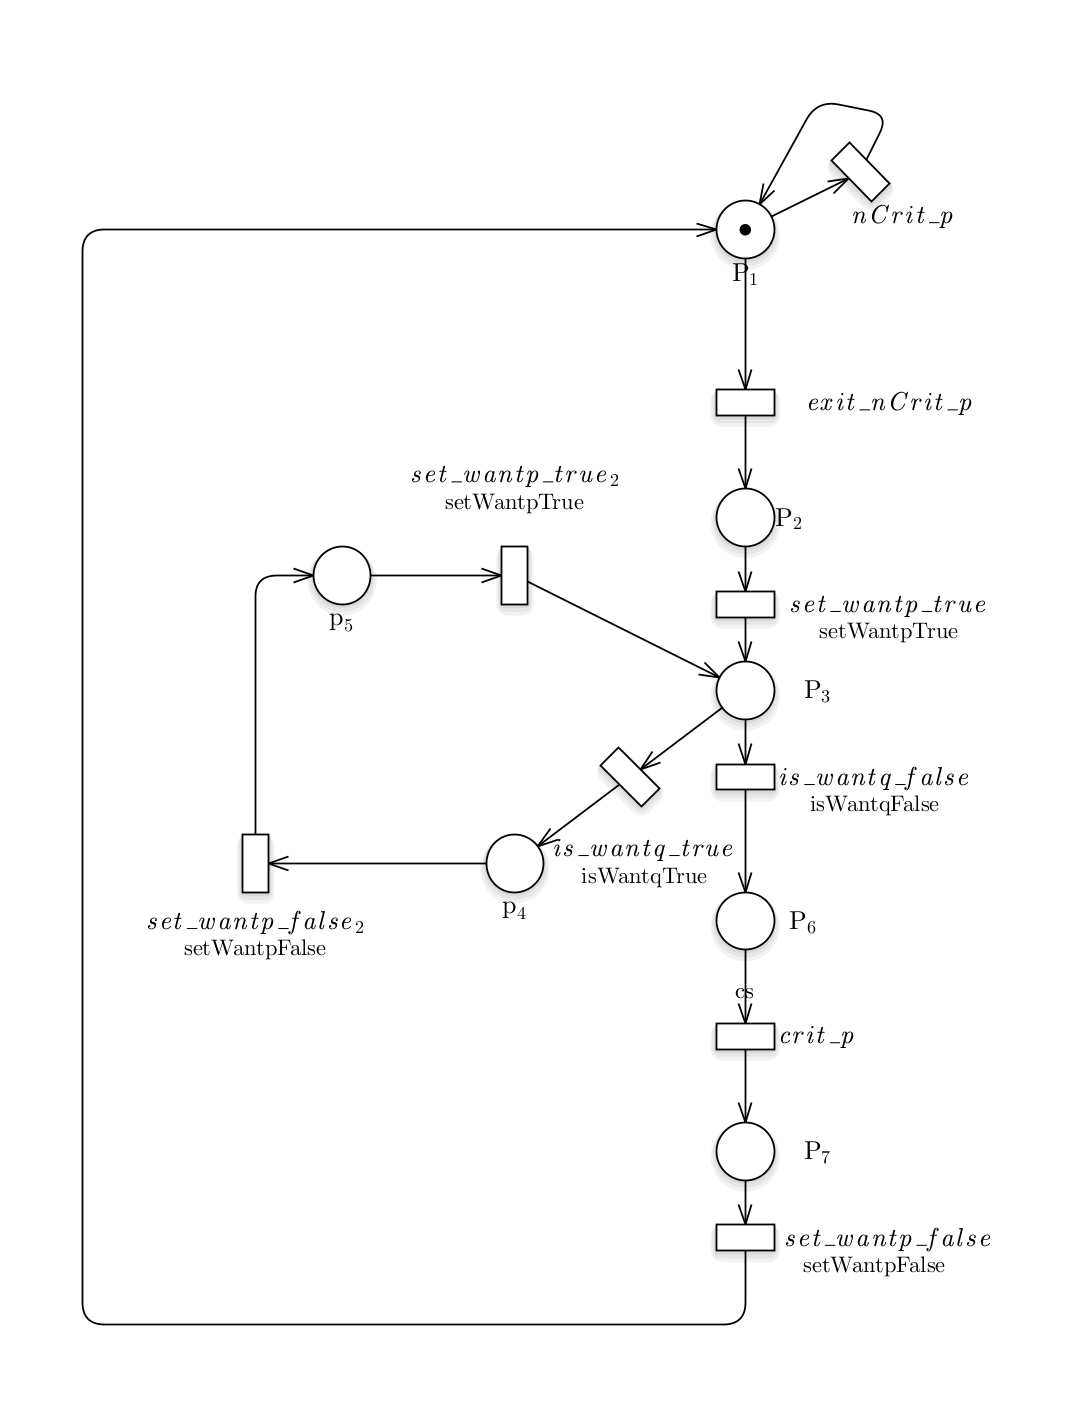
\includegraphics[width=0.4\textwidth]{p3.9.png}
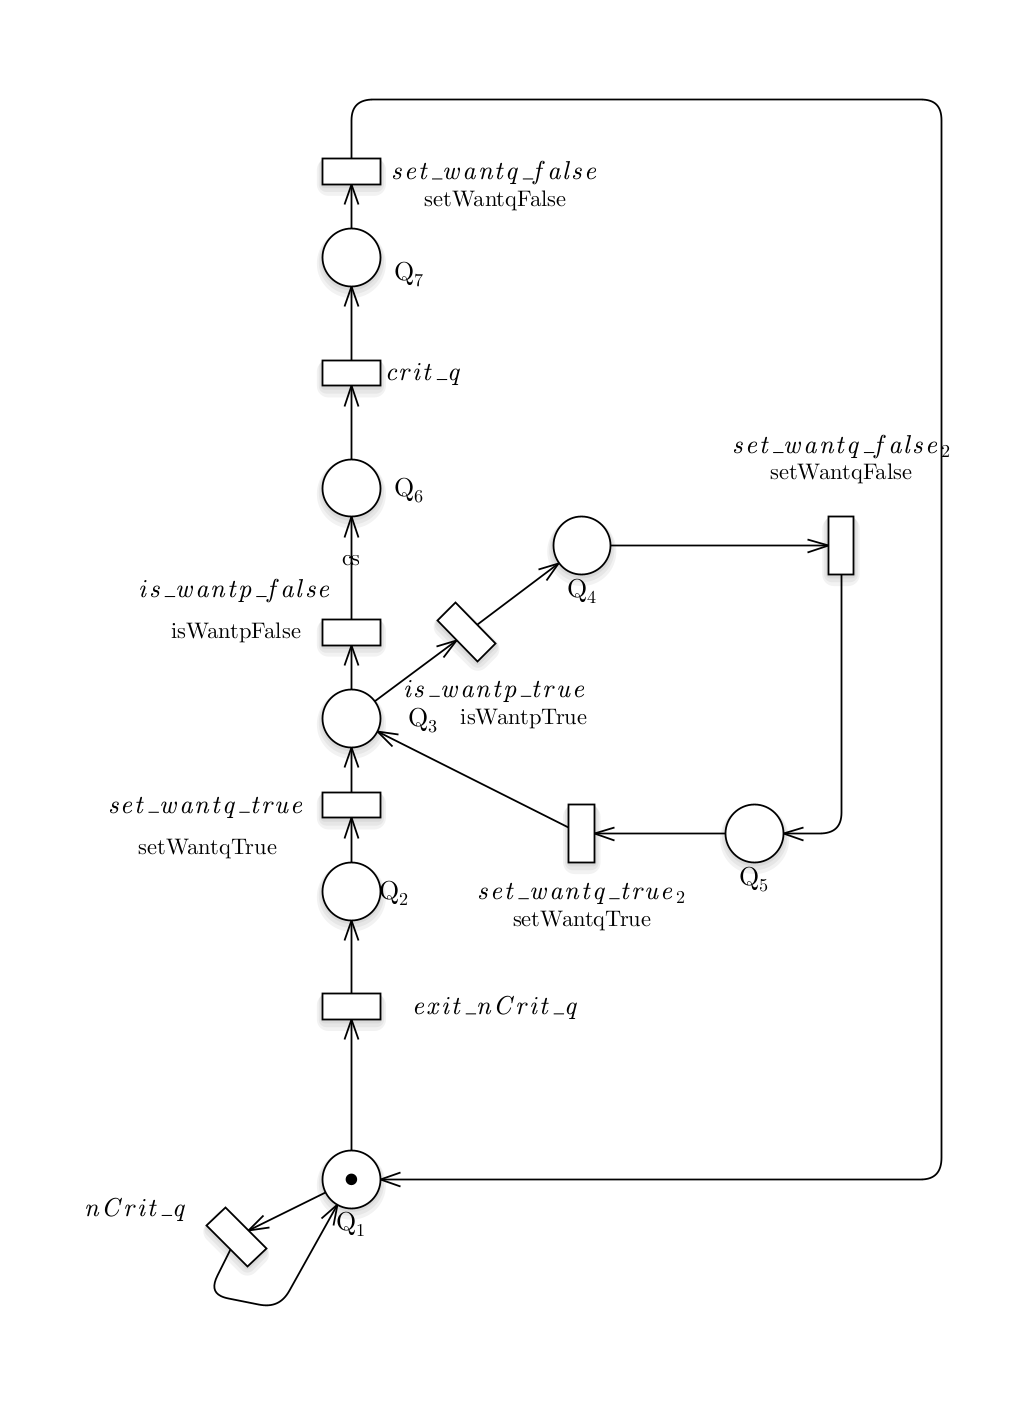
\includegraphics[width=0.4\textwidth]{q3.9.png}
}
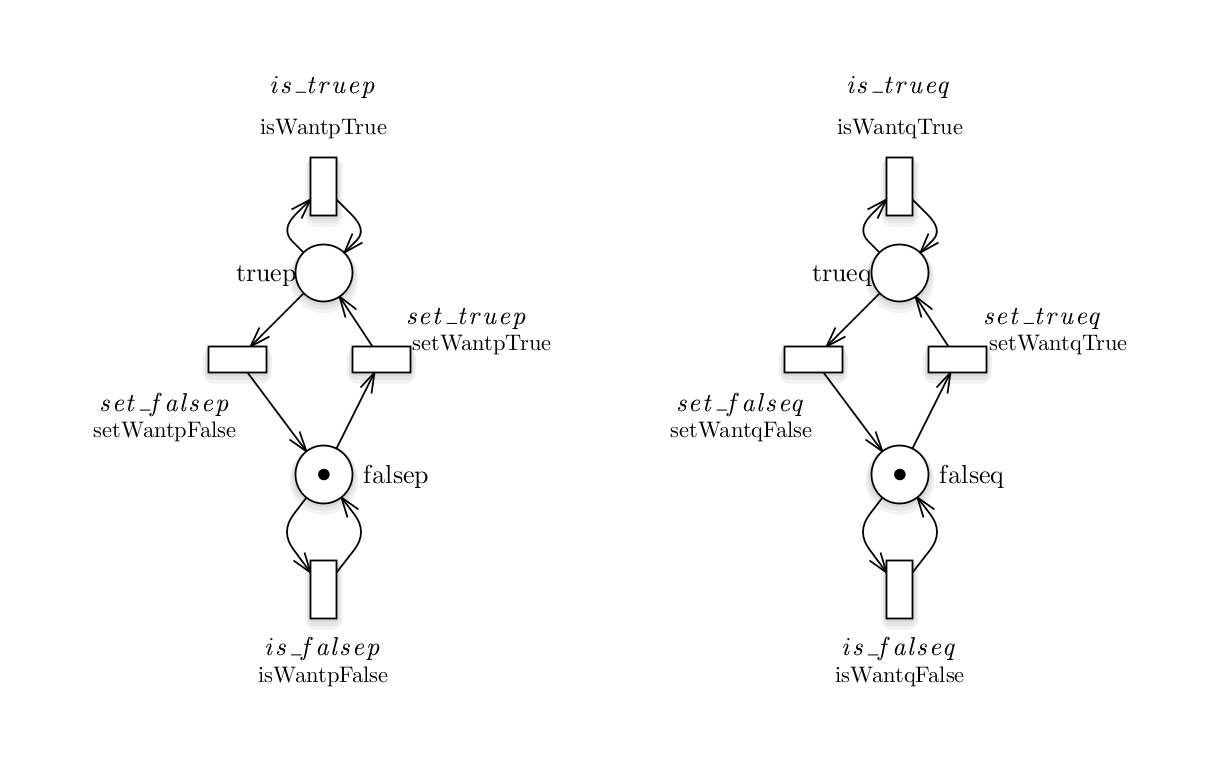
\includegraphics[width=0.8\textwidth]{variables.png}
\end{center}
\newpage
\begin{figure*}[!ht]
\centering
\makebox[\textwidth][c]{
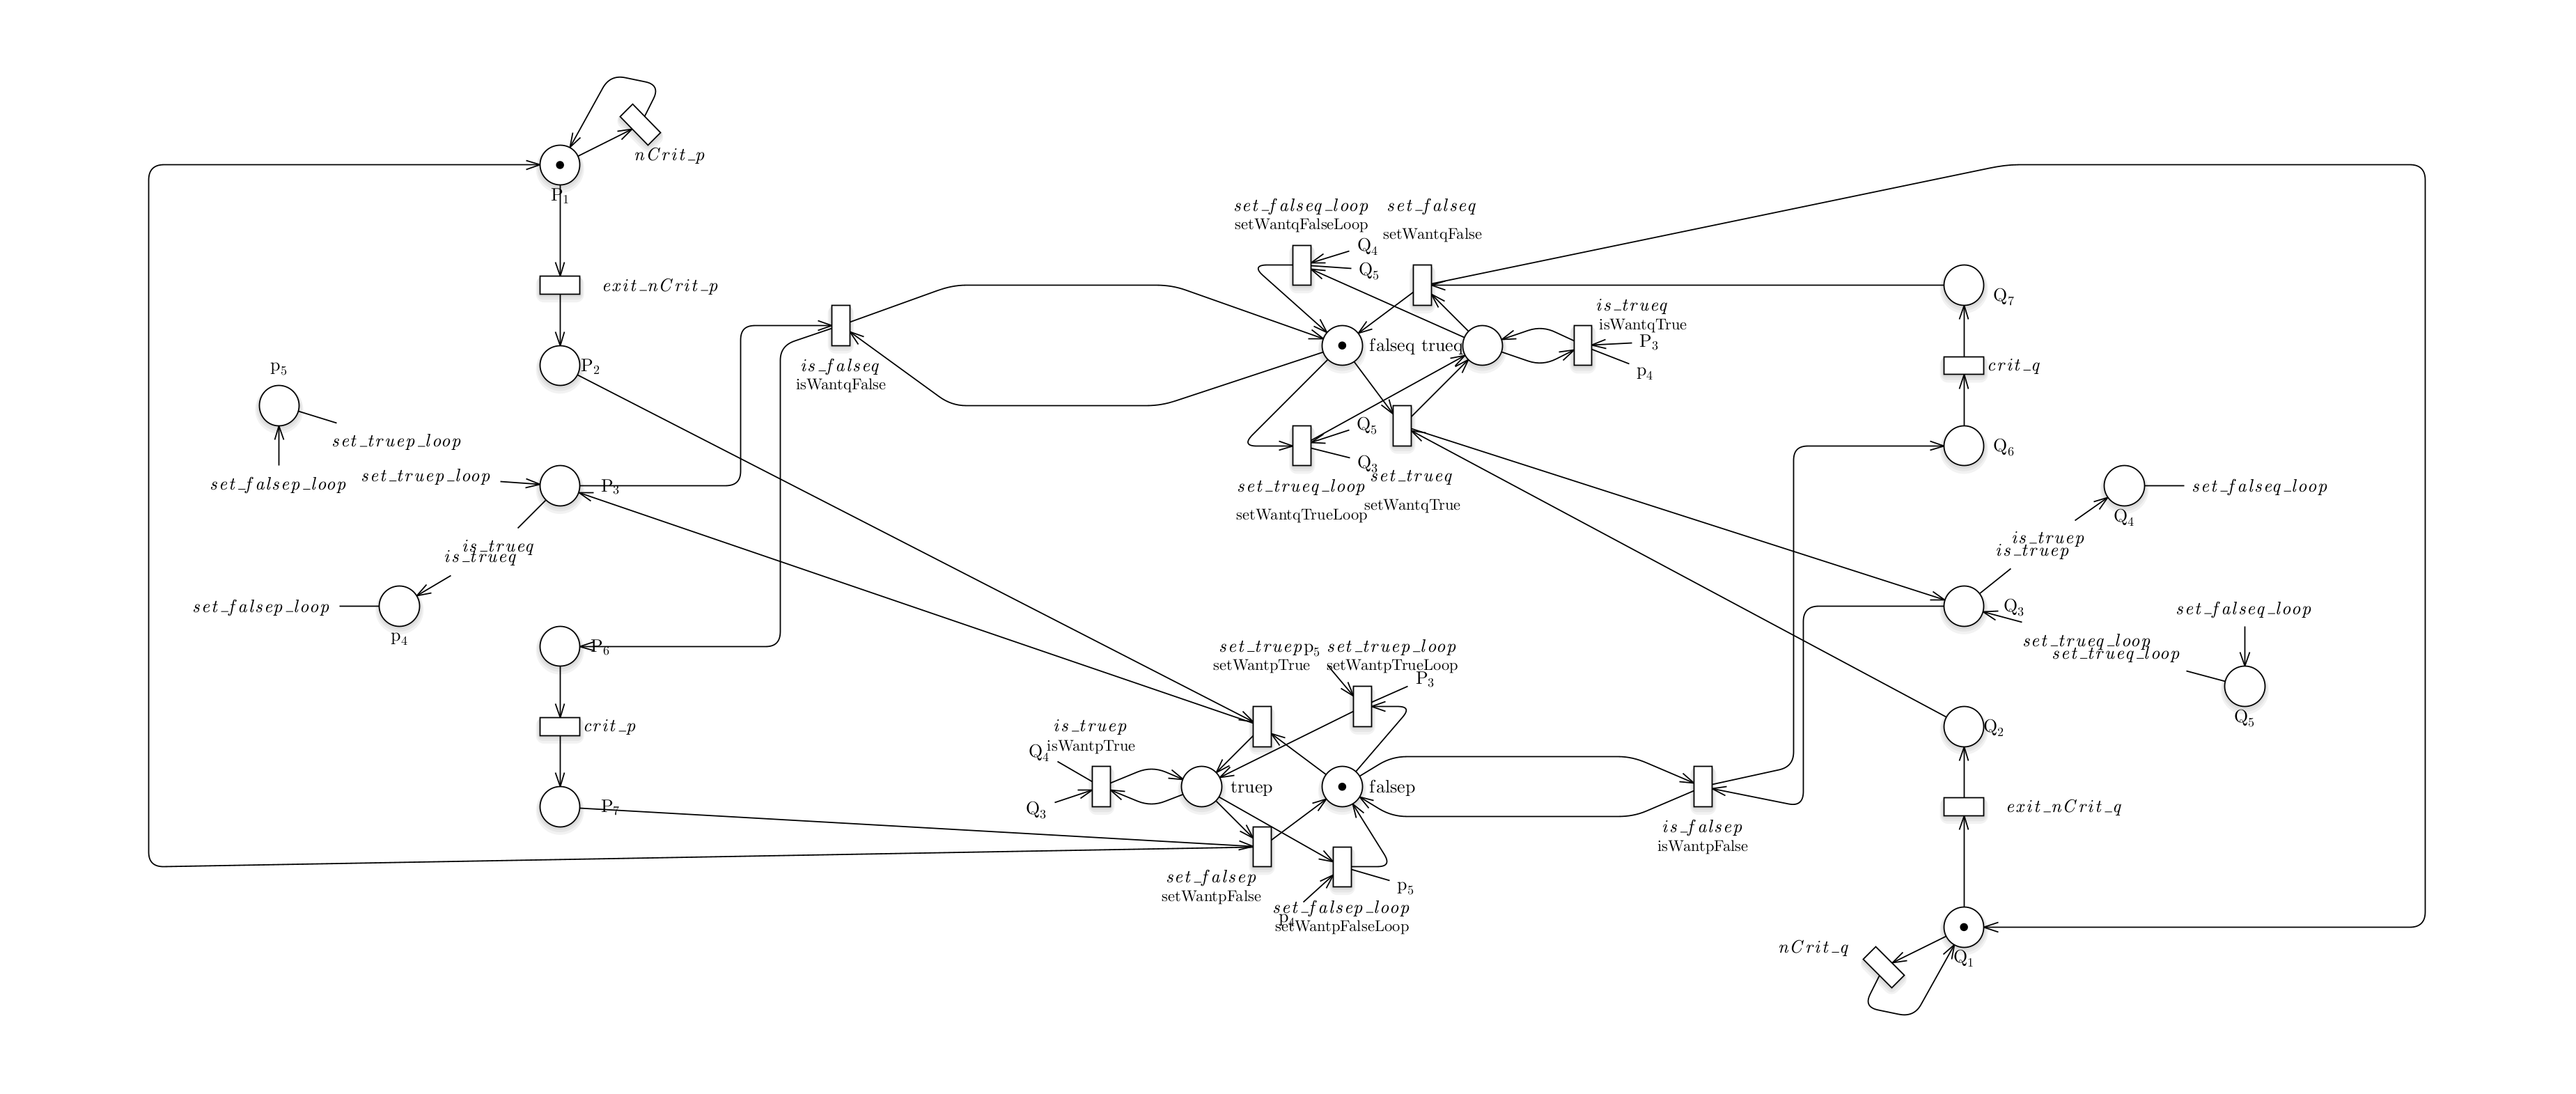
\includegraphics[width=1.6\textwidth]{3.9PN.png}}
\caption{Rete di petri composta} \label{FIG:3.9PN}
\end{figure*}
\newpage
\subsubsection{RG}
Il reachability graph, in figura \ref{FIG:3.9RG}, è composto da 45 stati, di cui nessuno rappresentante una situazione di Deadlock.
\begin{figure*}[!ht]
\centering
\makebox[\textwidth][c]{
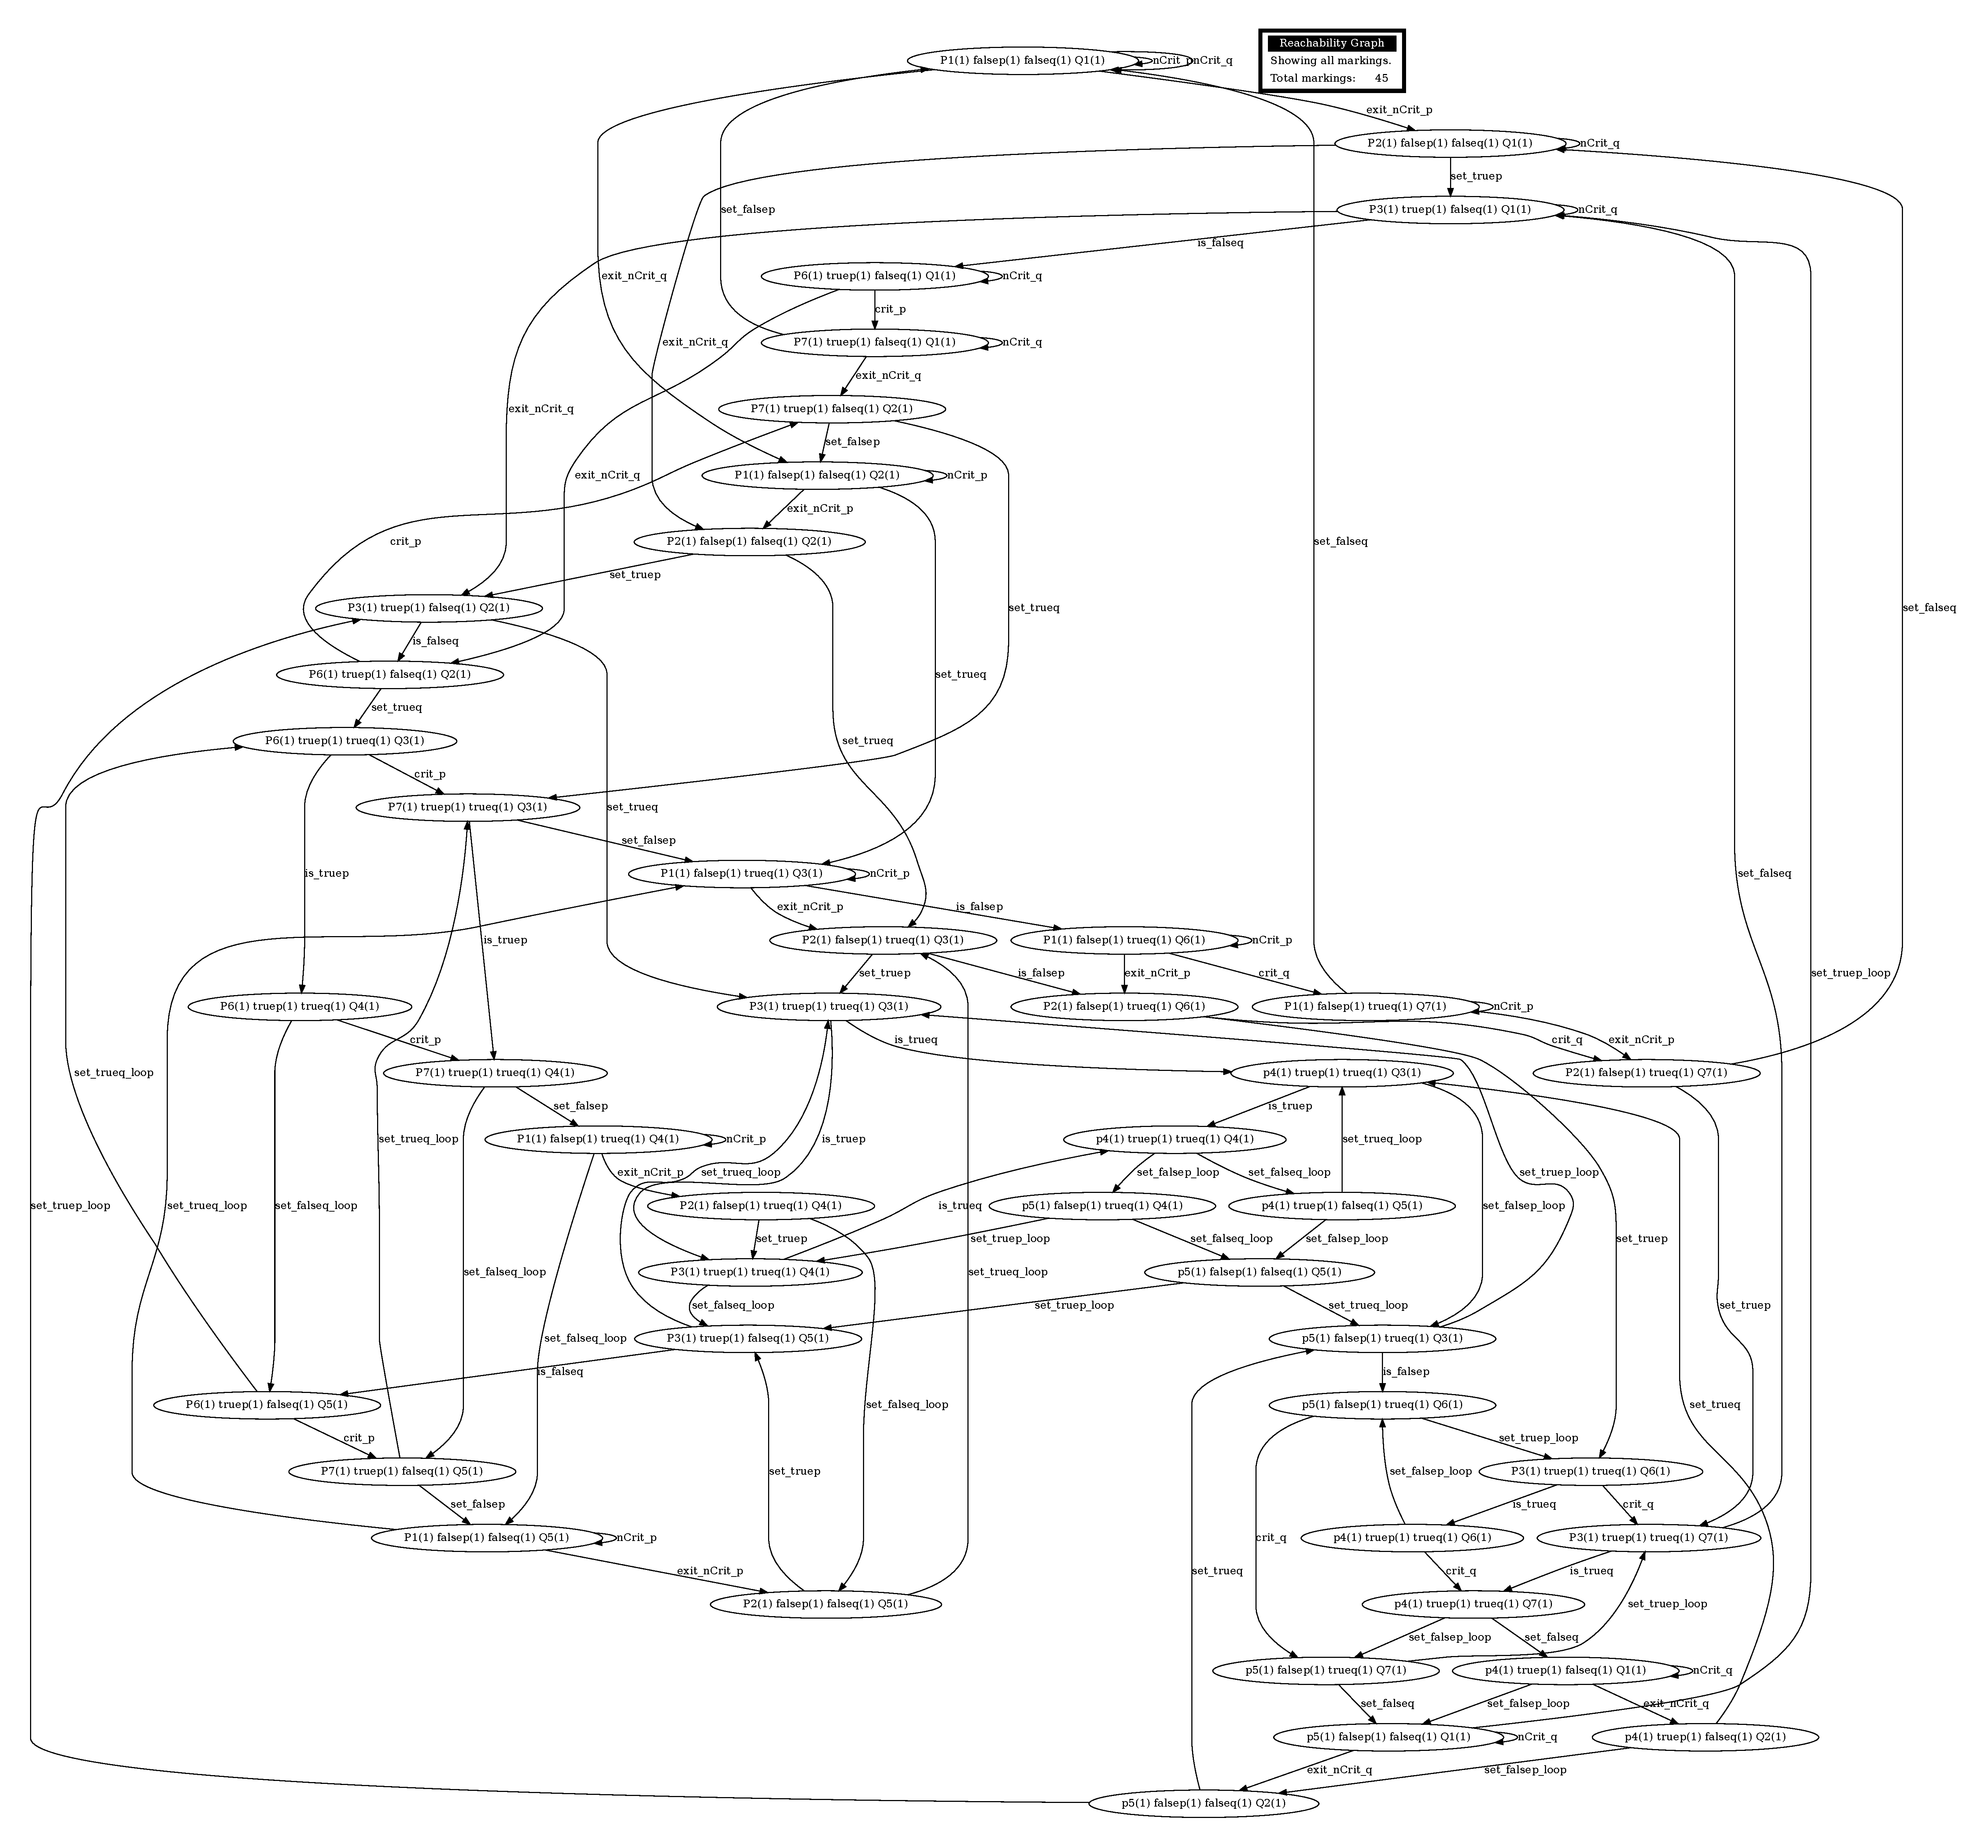
\includegraphics[width=1\textwidth]{3.9RG}}
\caption{Reachability graph 3.9} \label{FIG:3.9RG}
\end{figure*}
\newpage
\subsubsection{Analisi strutturale} 
\label{SEC:3_9_strutturale}
Il calcolo dei \textit{semiflow} fornisce 6 \textit{T-semiflow} minimali e 8 \textit{P-semiflow} minimali, lo studio dei P-invarianti rivela che tutti i posti sono 1-bound come negli altri casi e permette di affermare che le variabili p e q assumono un solo valore di verità.
Invece dallo studio dei \textit{T-semiflow} non emerge solo la \textit{liveness} (come prevedibile) ma è interessante notare la presenza dei \textit{T-semiflow} che interessano i posti [P3, P4, P5] e [Q3, Q4, Q5] cioè le esecuzioni del ciclo di \textit{P \textit{e} Q}.


\subsubsection{Model Checking GreatSPN}
Sono state verificate le seguenti formule CTL:
\begin{itemize}
	\item mutua esclusione: \textit{AG !(\#P6==1 \&\& \#Q6==1)} \textcolor{green}{true}.\\
		Il sistema rispetta la mutua esclusione.
	\item deadlock: \textit{AG AF ((\#P1==1) || (\#Q1 == 1))} \textcolor{red}{false}.\\
		Il sistema sembra andare in deadlock, il controesempio presentato dal Model Checker è l'esecuzione in cui entrambi i processi entrano nel loop di richiesta e si bloccano a vicenda l'uscita.\\
		Ma questo non è deadlock, è starvation, quindi la formula logica usata per controllare l'assenza di deadlock in questo caso va modificata.
	\item deadlock corretto: \textit{AG AF (((\#P1==1) || (\#Q1 == 1)) || ((\#P4==1) || (\#Q4 == 1)))} \textcolor{green}{true}.\\
		In questo modo viene controllato che i processi siano liberi di eseguire o il ciclo esterno (dallo stato 1 fino al ritorno in stato 1) o almeno quello interno (dallo stato 3 ritorno allo stato 3).
	\item assenza di starvation: \textit{AG((\#P2 >0 ) -> (AF \#P6>0 ))} ed anche \textit{AG((\#P2 >0 ) -> (AF \#P6>0 ))}. Entrambe risultano \textcolor{red}{false}.\\
		Come anticipato prima si può verificare starvation. Sia perchè un processo riesce sempre ad entrare in CS escludendo l'accesso all' altro (situazione mostrata come controesempio dal Model Checker) oppure perchè entrambi i processi si bloccano a vicenda l'accesso.
\end{itemize}
Sono state verificate le seguenti formule LTL:
\begin{itemize}
	\item mutua esclusione: \textit{G !(\#P4==1 \&\& \#Q4==1)} \textcolor{green}{true}.
	\item assenza di starvation: \textit{G F (\#P2==1) -> G F(\#P6 == 1)} ed anche \textit{G F (\#Q2==1) -> G F(\#Q6 == 1)}. Entrambe risultano \textcolor{red}{false}.
	\item deadlock: \textit{G F( (\#P1 ==1) ||  (\#Q1 ==1))} \textcolor{red}{false}.
	\item deadlock corretto: \textit{G F ( (\#P1==1) || (\#Q1 == 1) ) || G F ((\#P4==1) || (\#Q4 == 1)))} \textcolor{green}{true}.\\
\end{itemize}
\newpage
\subsection{NuSMV}
L'implementazione del sistema tramite il linguaggio di NuSMV non presenta particolari differenze rispetto allo pseudocodice 3.9. Allo stato 5 vi è il salto che permette di creare il ciclo interno e si può uscire da questo ciclo solamente se la variabile \textit{want\_other} è falsa quando il processo è nello stato s3.
\lstinputlisting{figures/3_9_code.smv}
Il comando \texttt{print\_reachable\_states} mostra 45 stati raggiungibili di 196 possibili, in linea con la dimensione del Reachability Graph.
Non è presente alcuno stato di deadlock.
\newpage
\subsubsection{Model Checking NuSMV}
Sono state verificate le seguenti formule CTL:
\begin{itemize}
        \item mutua esclusione: \textit{AG !(( p.state = s6 ) \& (q.state = s6 ))} \textcolor{green}{true}.
        \item deadlock: \textit{AG AF (( p.state = s1 )| ( q.state = s1 ))} \textcolor{red}{false}.\\
		Si verifica di nuovo la stesso situazione presentata in GreatSPN, la formula è incorretta per verificare l'assenza di deadlock. Va quindi riscritta.
        \item deadlock corretto: \textit{AG AF ((( p.state = s1 ) | ( q.state = s1 ) ) | (( p.state = s4 ) | ( q.state = s4 ) ))} \textcolor{green}{true}.
        \item assenza di starvation: \textit{AG (( p.state = s2 ) -> (AF p.state = s3 ))} ed anche \textit{AG (( q.state = s2 ) -> (AF q.state = s3 ))}. Entrambe risultano \textcolor{red}{false}.\\
		Come visto nel Model Checking in GreatSPN si può verificare starvation sia perchè un processo blocca l'altro e va solo lui in critical section ma anche perchè entrambi si bloccano l'accesso a vicenda.
		Il controesempio fornito dal MC è una istanza del secondo tipo.
\end{itemize}
Sono state verificate le seguenti formule LTL:
\begin{itemize}
        \item mutua esclusione: \textit{G !(p.state = s4 \& q.state = s4)} \textcolor{green}{true}.
        \item deadlock: \textit{G F(( p.running) | ( q.running ) )} \textcolor{green}{true}. \\
		In questo caso il problema di definizione della formula logica "il processo può essere eseguito" non si pone, in quanto NuSMV permette di utilizzare la clausola \texttt{running} per stabilire se un processo sta venendo eseguito o no (questo solo in LTL).\\
		Quindi il Model Checker mostra correttamente l'assenza di Deadlock.
        \item assenza di starvation: \textit{G (p.state = s2 ->  F p.state = s3)} ed anche \textit{G (p.state = s2 ->  F p.state = s3)}. Entrambe risultano \textcolor{red}{false}.\\
		L'esempio presentato dal Model Checker è lo stesso dell'analisi con CTL.
\end{itemize}

\newpage
\section{Algoritmo 3.10}
\label{SEC:3.10}
\begin{center}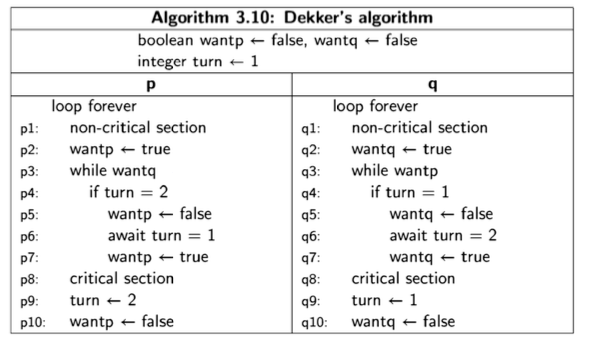
\includegraphics[width=1\textwidth]{3.10.png}\end{center}
L'algoritmo in figura risolve il problema della starvation dell'algoritmo 3.9 \ref{SEC:3.9} sfruttando l'idea dell'algoritmo 3.2 \ref{SEC:3.2} di inserire una variabile turn per decidere quale processo entrerà in sezione critica.
A differenza del 3.2 però il controllo del turno viene effettuato solamente se c'è effettivamente qualcun'altro in attesa di entrare in sezione critica.\\

Per ogni operazione effettuabile sulle variabili è stata aggiunta una nuova transizione alle stesse.
Quindi la variabile \textit{wantP} avrà due transizioni atte al settarla vera o falsa, una usata fuori dal ciclo interno ed una all'interno (transizione \texttt{set\_truep}).
Stesso discorso vale per la variabile turn. A differenza di quella presentata in sezione \ref{SEC:3.2}
\subsection{Disclaimer}
\disclaimer{Questo algoritmo non dovrebbe soffrire di starvarion, invece la sua implementazione in Petri net ne soffre. Questo è effettivamente un \textit{tranello} della prof. Vuole che vi rendiate conto della cosa e, per quanto non sia impossibile generare un PN con un arbitraggio che rende fair il modello, basta che all'esame le dite ciò.\\
Insomma quello che ho fatto io è andato bene, le ho spiegato che non avevo trovato il modo e lei mi ha risposto qualcosa sulla falsa riga di "non mi aspettavo lo trovaste, mi aspettavo mi chiedeste aiuto"}
\subsection{Rete di Petri}
\begin{center}
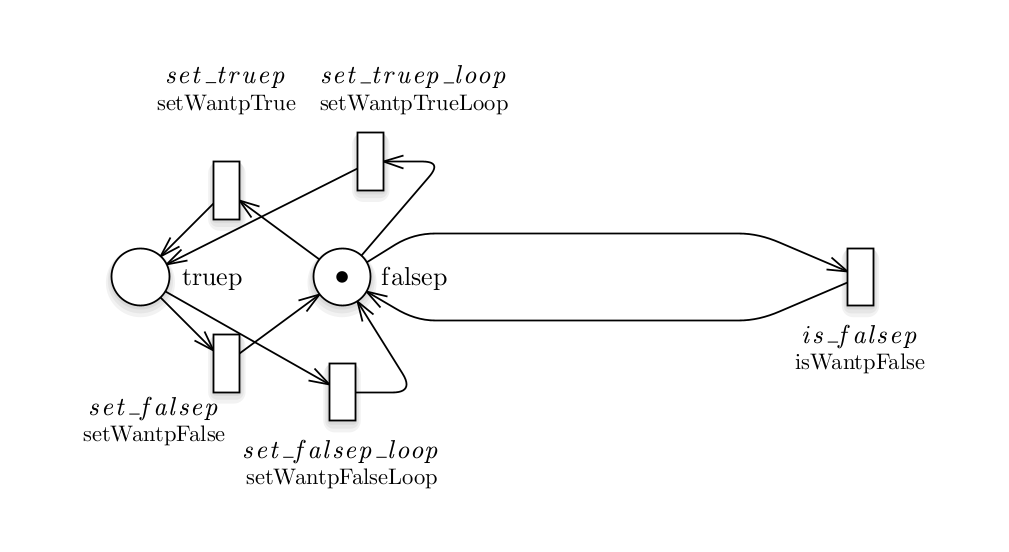
\includegraphics[width=0.7\textwidth]{WantP.png}
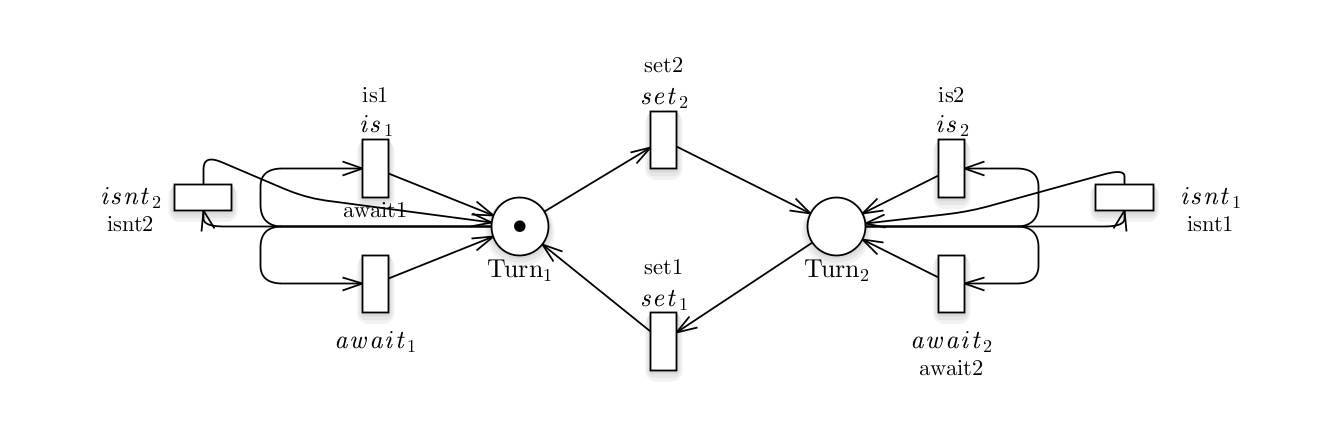
\includegraphics[width=0.8\textwidth]{turn.png}\\
Variabili \textit{P \textit{e} Q} e variabile \textit{Turn}
\end{center}
\begin{center}
\makebox[\textwidth][c]{
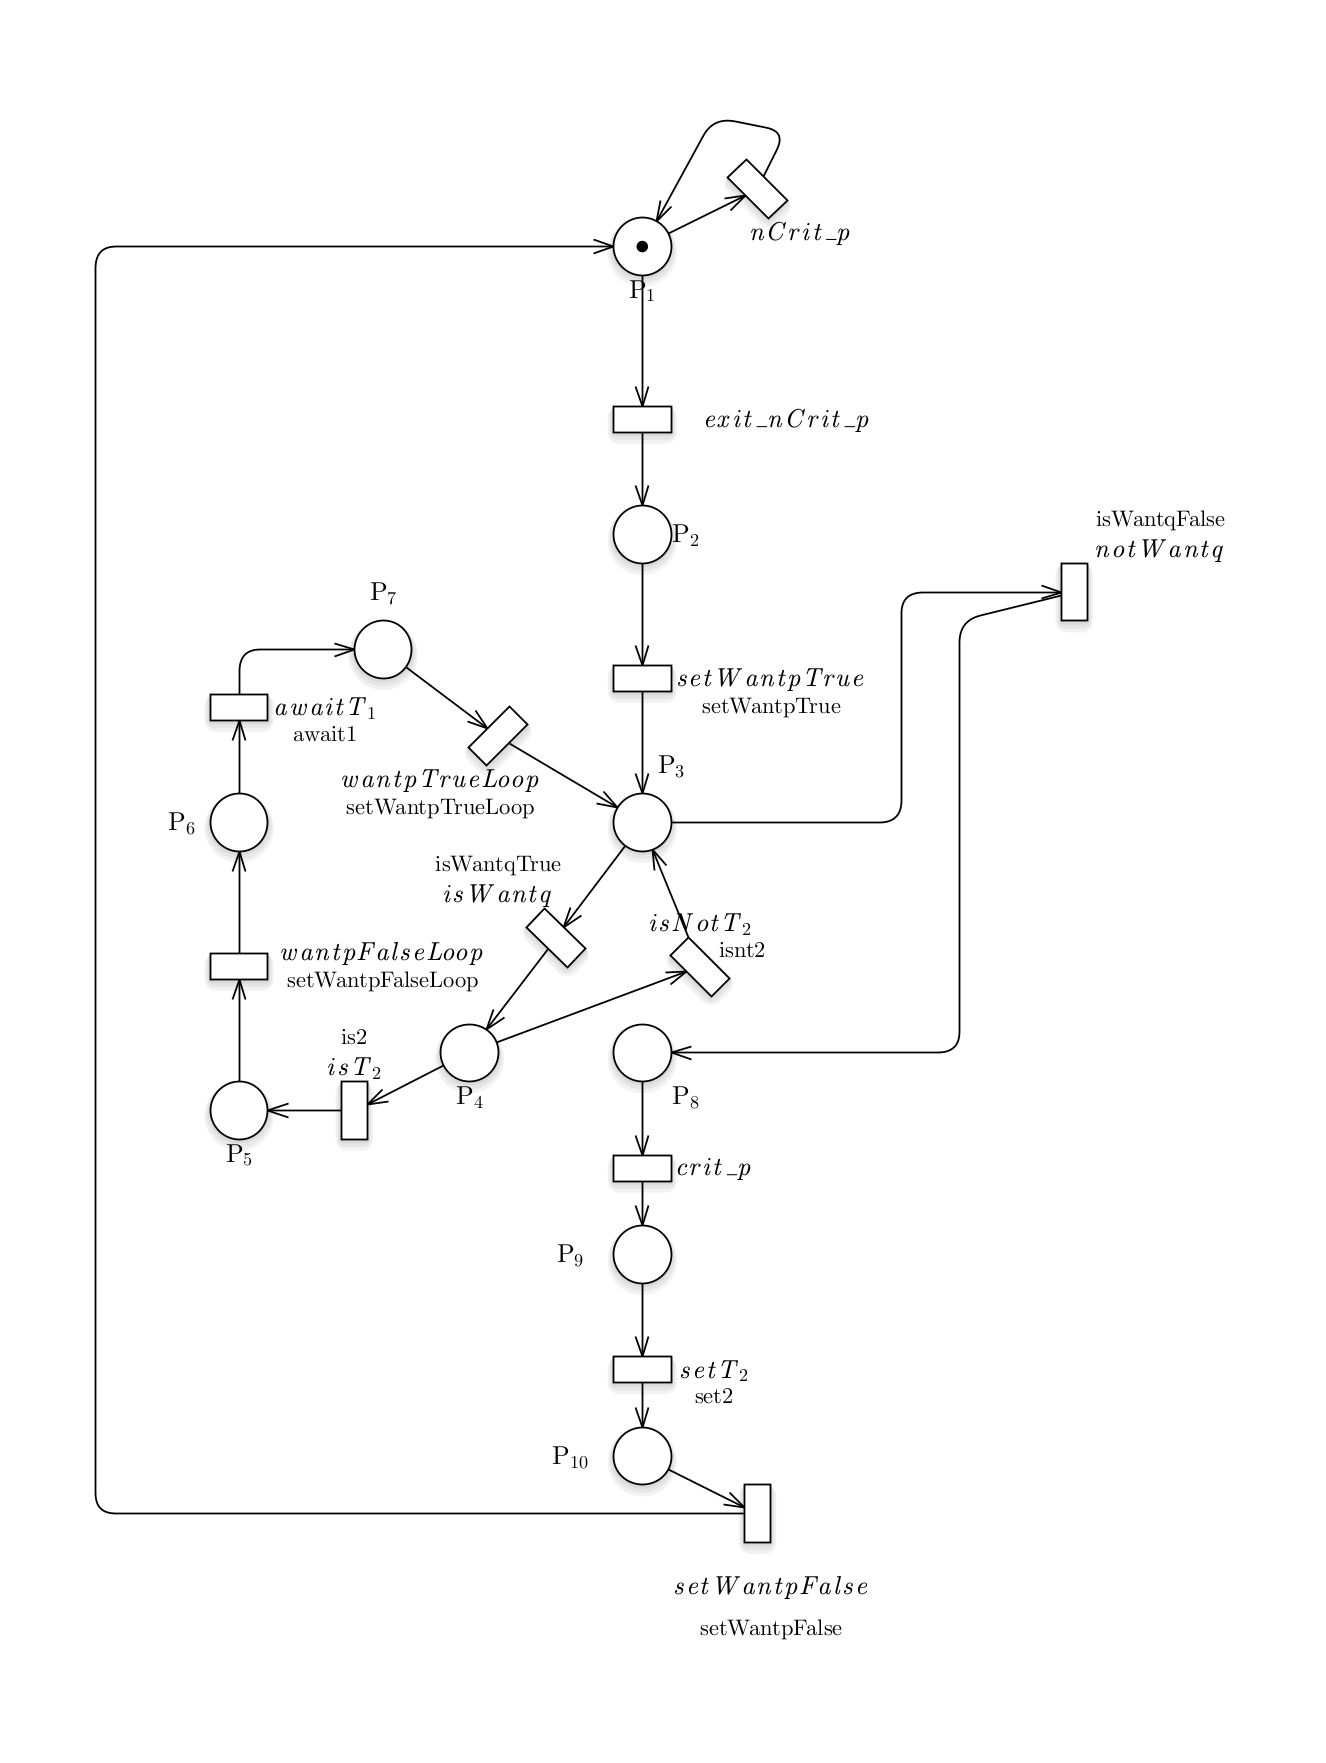
\includegraphics[width=0.8\textwidth]{3.10p.png}
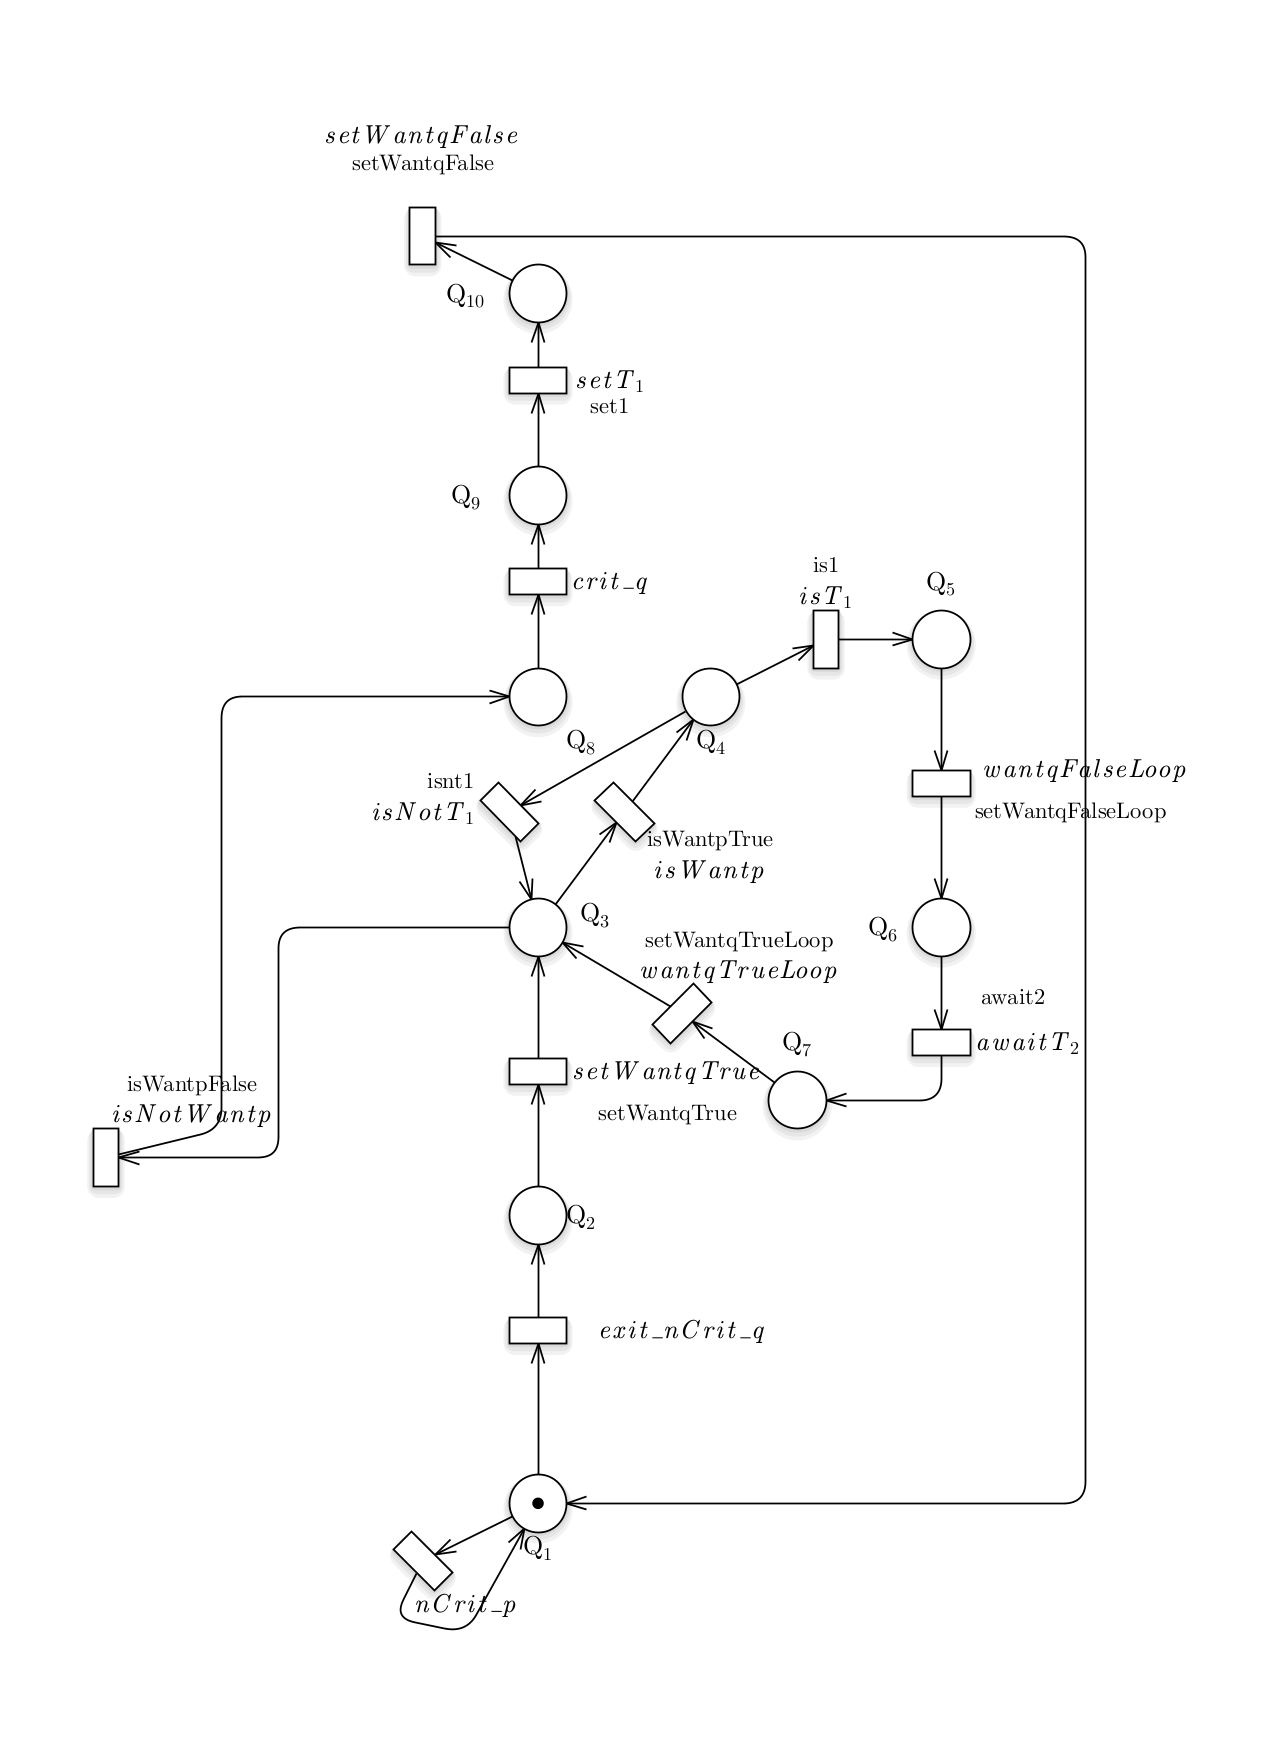
\includegraphics[width=0.8\textwidth]{3.10q.png}}
Processi \textit{P \textit{e} Q}
\end{center}
\newpage
\begin{figure*}[!ht]
\centering
\makebox[\textwidth][c]{
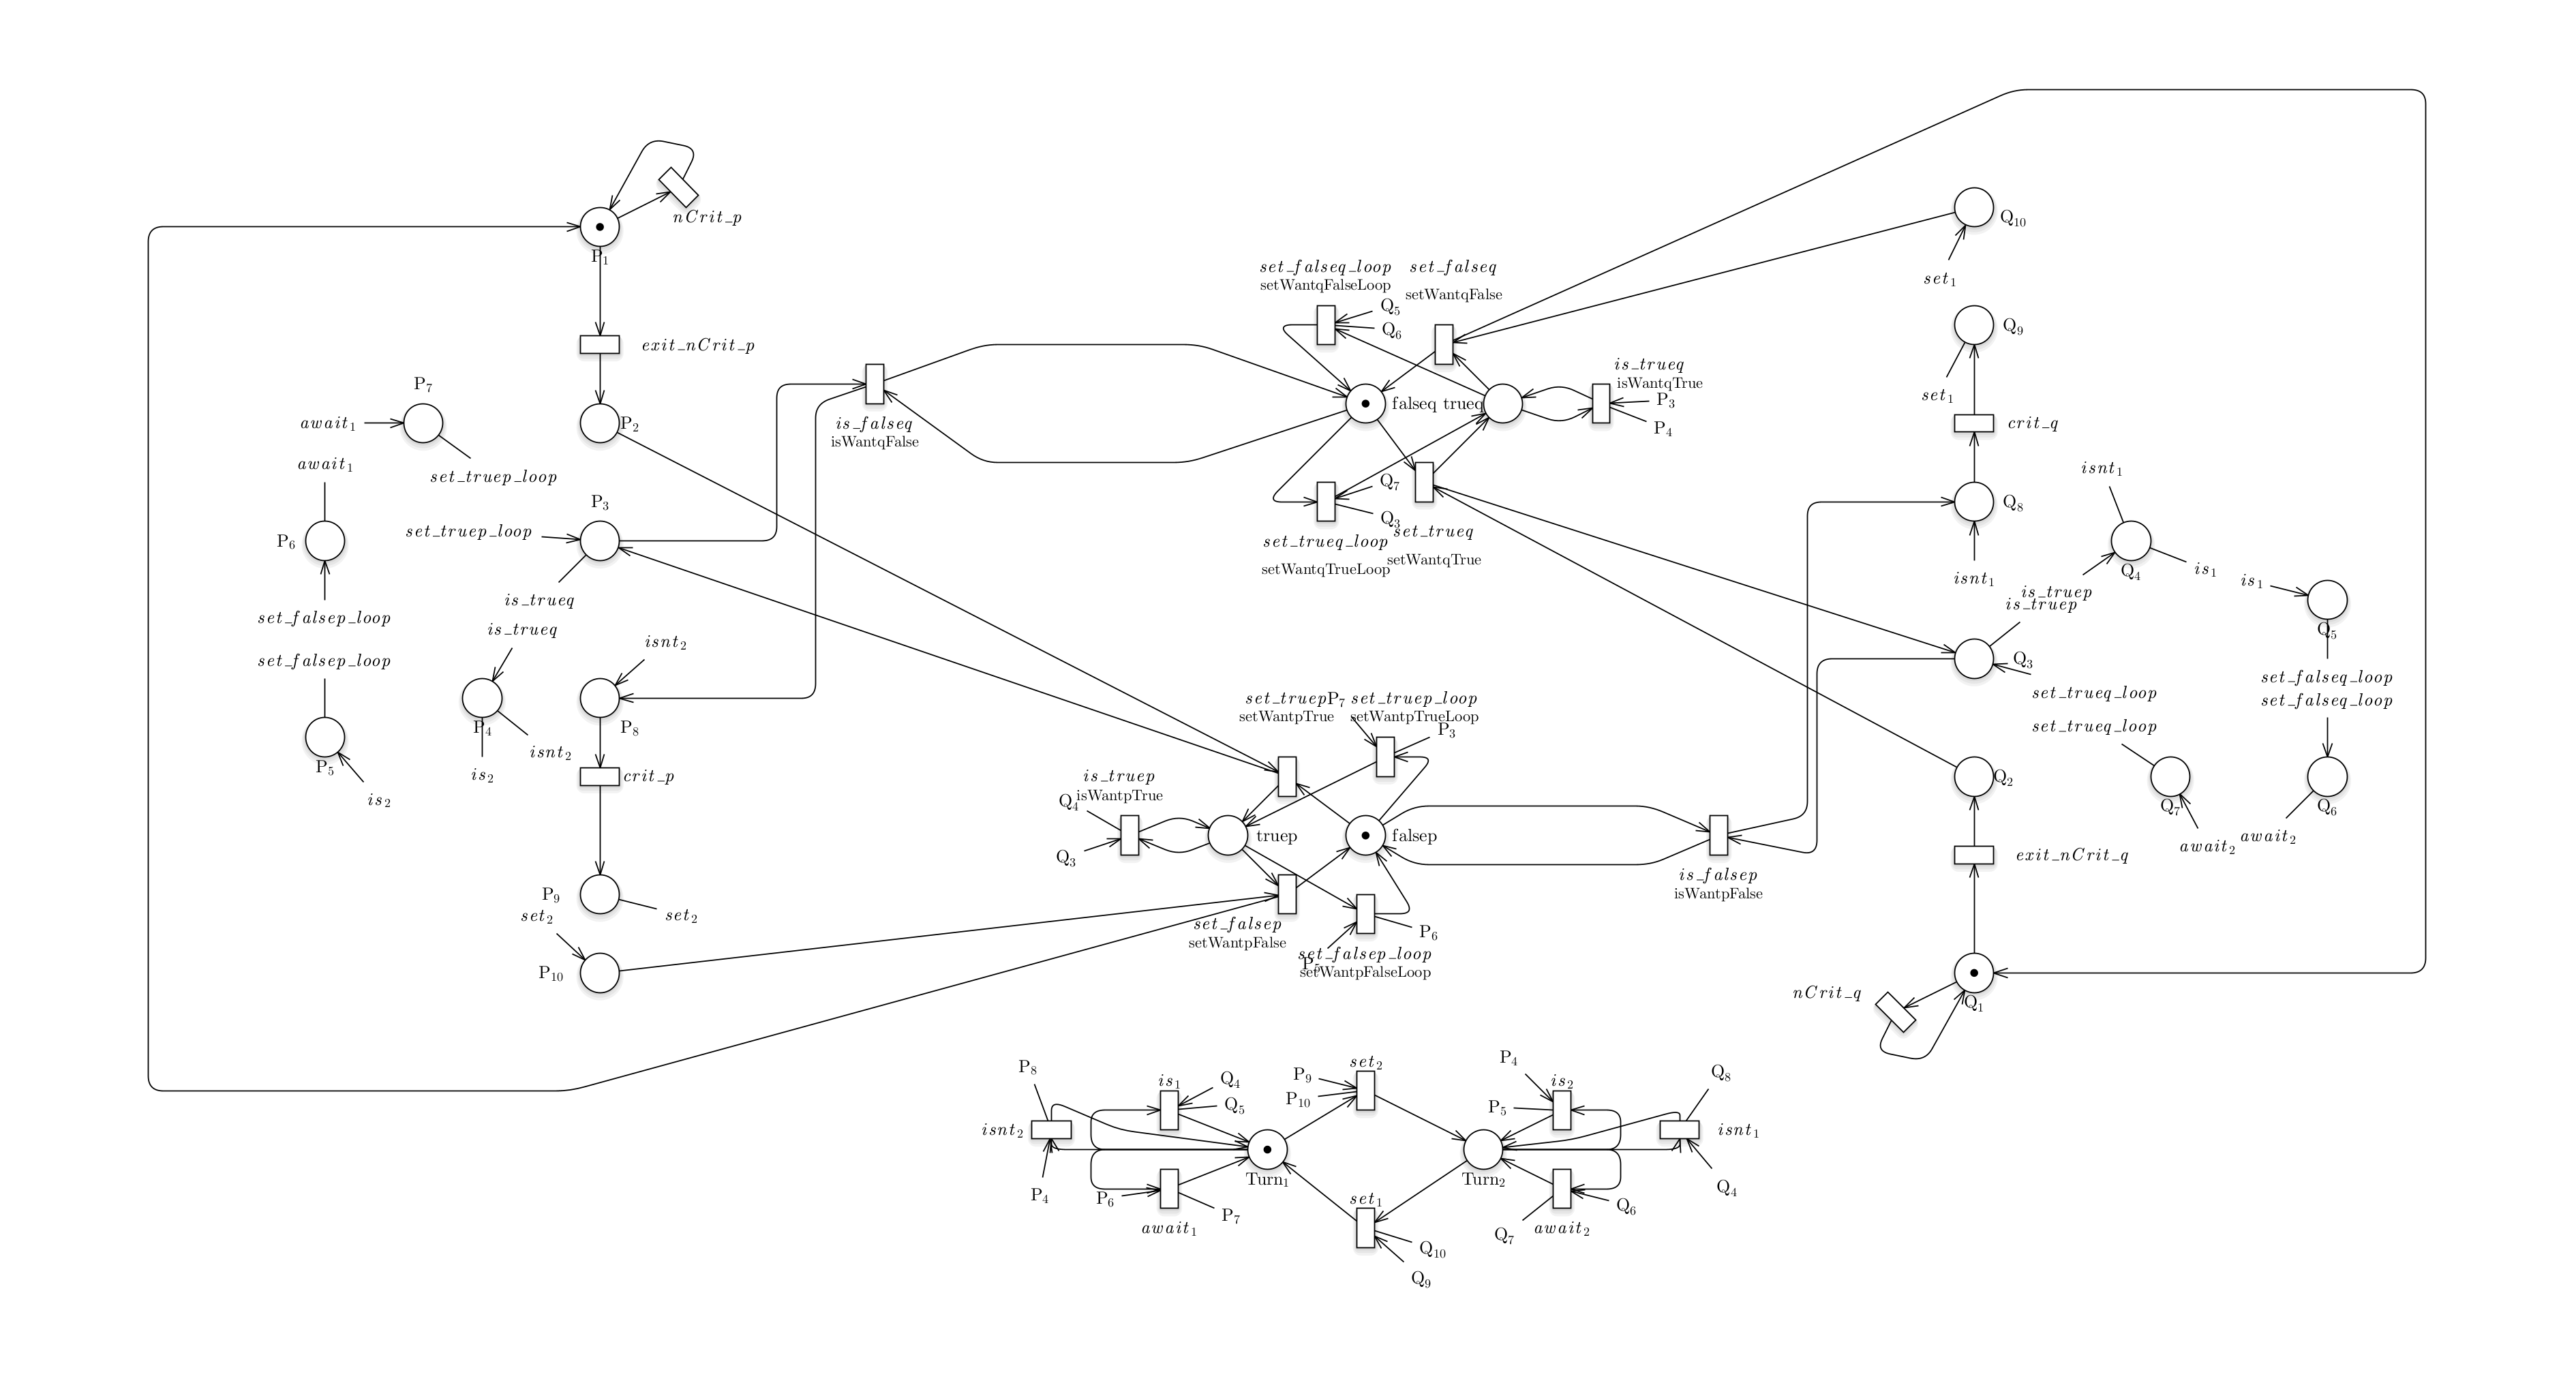
\includegraphics[width=1.6\textwidth]{3.10PN.png}}
\caption{Rete di petri composta} \label{FIG:3.10PN}
\end{figure*}
\newpage
\subsubsection{RG}
Il reachability graph, in figura \ref{FIG:3.10RG}, è composto da 134 stati, di cui nessuno rappresentante una situazione di Deadlock.
\begin{figure*}[!ht]
\centering
\makebox[\textwidth][c]{
\includegraphics[width=1\textwidth]{3.10RG}}
\caption{Reachability graph 3.10} \label{FIG:3.10RG}
\end{figure*}
\newpage
\subsubsection{Analisi strutturale}
In quest'ultimo caso possiamo identificare 9 \textit{P-semiflow} minimali e 7 \textit{T-semiflow} minimali. 
Le variabili $P$ e $Q$ possono assumere un solo valore di verità ed la marcatura della varibile $Turn $ può essere solamente nel posto $Turn_1$ o alternativamente nel posto $Turn_2$. 
Come negli altri casi il sistema è 1-bound.\\
L'analisi dei \textit{T-semiflow} mostra che il sistema possiede la proprietà di \textit{liveness} ed è interessante analizzarne 3.
Come nel caso precendete (sezione \ref{SEC:3_9_strutturale}) sono presenti due semiflow che corrispondono ai cicli ma a differenza di tutti i casi precedenti sono assenti i semiflow che coinvolgono separatamente tutti i posti di $P$ e tutti i posti di $Q$.
Vi è invece un unico flow che interessa tutti i posti di entrambi i processi, è quindi possibile attraverso una esecuzione dei due processi ritornare allo stato iniziale, questo rende la rete una rete \textbf{consistente}.

\subsubsection{Model Checking GreatSPN}
Sono state verificate le seguenti formule CTL:
\begin{itemize}
	\item mutua esclusione: \textit{AG !(\#P8==1 \&\& \#Q8==1)} \textcolor{green}{true}.
	\item assenza di starvation: \textit{AG((\#P3 >0 ) -> (AF \#P8>0 ))} ed anche \textit{AG((\#Q3 >0 ) -> (AF \#Q6>0 ))}. Entrambe risultano \textcolor{red}{false}.\\
		Il motivo di questa incongruenza è dovuto ad un errore nei fairness constraint (\textit{\#P2 > 0 || \#Q2 > 0}).Infatti questi non escludono la possibilità che un processo rimanga in uno stato relativo alla richiesta della sezione critica e l'esecuzione viene concessa solo all'altro processo che cicla in sezione non critica.Questa computazione non fair deve essere gestita in altro modo.
	\item assenza di starvation imponendo progresso in regione non critica: Fairness constraint \textit{\#P2 > 0 || \#Q2 > 0}. Entrambe risultano \textcolor{green}{true}.\\
		Un modo di imporre una computazione fair è garantire il progresso del processo opposto a quello di cui si vuole verificare l'assenza di starvation. La proposizione \textit{(\#Q2 ==1 )} ad esempio garantisce che il proceso \textit{Q} uscirà dalla sezione non critica e tenterà l'accesso in \textit{cs}, riuscendo ad acceddere o permettendo l'esecuzione di \textit{P}. In tal modo però i processi sono obbligati al progresso in sezione non critica.
		Un' implementazione alternativa consiste nella creazione di un arbitro che assegni il \textit{quanto} di tempo di esecuzione ai processi a seconda di come viene costruito, di fatto specificando la politica di scheduling.
	\item deadlock: \textit{AG AF ((\#P1==1) || (\#Q1 == 1))} \textcolor{green}{true}.
\end{itemize}
Sono state verificate le seguenti formule LTL:
\begin{itemize}
	\item mutua esclusione: \textit{G !(\#P8==1 \&\& \#Q8==1)} \textcolor{green}{true}.
	\item assenza di starvation: \textit{G F (\#P3==1) -> G F(\#P8 == 1)} ed anche \textit{G F (\#Q3==1) -> G F(\#Q8 == 1)}. Entrambe risultano \textcolor{red}{false}.\\
	In questo caso si verifica starvation, anche se non dovrebbe succedere. Ciò è dovuto ai \textit{fairness constraint}.Non è infatti vero che se un processo richiede l'accesso in sezione critica, poichè potrebbe avvenire una computazione non fair in cui il processo che richiede l'accesso rimane bloccato su uno qualsiasi dei posti \textit{3, ..., 8} mentre l'altro processo prosegue in sezione non critica.
	\item assenza di starvation imponendo progresso in regione non critica: \textit{G F ( \#Q2 ==1 ) -> (G F (\#Q3==1) -> G F(\#Q8 == 1))} E la proposizione corrispondente per Q risultano \textcolor{green}{true}.\\
		Un modo di imporre una computazione fair è garantire il progresso del processo opposto a quello di cui si vuole verificare l'assenza di starvation. La proposizione \textit{(\#Q2 ==1 )} ad esempio garantisce che il proceso \textit{Q} uscirà dalla sezione non critica e tenterà l'accesso in \textit{cs}, riuscendo ad acceddere o permettendo l'esecuzione di \textit{P}. In tal modo però i processi sono obbligati al progresso in sezione non critica.
		Un' implementazione alternativa consiste nella creazione di un arbitro che assegni il \textit{quanto} di tempo di esecuzione ai processi a seconda di come viene costruito, di fatto specificando la politica di scheduling.
	\item deadlock: \textit{G F( (\#P1 ==1) ||  (\#Q1 ==1))} \textcolor{green}{true}.
\end{itemize}
\newpage
\subsection{NuSMV}
\lstinputlisting{figures/3_10_code.smv}
Il comando \texttt{print\_reachable\_states} mostra 134 stati raggiungibili di 800 possibili, in linea con la dimensione del Reachability Graph.
Non è presente alcuno stato di deadlock.\\

\subsubsection{Model Checking NuSMV}
Sono state verificate le seguenti formule CTL:
\begin{itemize}
        \item mutua esclusione: \textit{AG !(( p.state = s8 ) \& (q.state = s8 ))} \textcolor{green}{true}.
        \item assenza di starvation: \textit{AG (( p.state = s3 ) -> (AF p.state = s8 ))} ed anche \textit{AG (( q.state = s3 ) -> (AF q.state = s8 ))}. Entrambe risultano \textcolor{green}{true}.
        \item assenza di deadlock: \textit{AG AF (( p.state = s1 )| ( q.state = s1 ))} \textcolor{green}{true}.
\end{itemize}
Sono state verificate le seguenti formule LTL:
\begin{itemize}
        \item mutua esclusione: \textit{G !(p.state = s8 \& q.state = s8)} \textcolor{green}{true}.\\
        \item assenza di starvation: \textit{G (p.state = s3 ->  F p.state = s8)} ed anche \textit{G (p.state = s3 ->  F p.state = s8)}. Entrambe risultano \textcolor{green}{true}.\\
		A differenza del model checker di \textit{GreatSPN, NuSMV} implementa la possibilità di selezionare uno scheduler fair tramite il comando \texttt{FAIRNESS running}, non vi è quindi necessità di inserire constraint nella proposizione.
        \item assenza di deadlock: \textit{G F(( p.running) | ( q.running ) )} \textcolor{green}{true}. 
\end{itemize}

\section{Confronto}
Come si può notare dalla seguente tabella non è presente nessuna differenza tra le implementazioni effettuate con GreatSPN e le implementazioni in NuSMV.
\begin{center}
\makebox[\textwidth][c]{
\begin{tabular}{c|ccc|ccc|}
\cline{2-7}
		       & &  GreatSPN                                   &  & &                NuSMV                        &  \\ \cline{2-7}
		       & \multicolumn{1}{l|}{Stati raggiungibili} & \multicolumn{1}{l|}{Assenza di deadlock} & Mutua esclusione & \multicolumn{1}{l|}{Stati raggiungibili} & \multicolumn{1}{l|}{Assenza di deadlock} & Mutua esclusione  \\ \hline
	\multicolumn{1}{|l|}{3.2} & \multicolumn{1}{l|}{16} & \multicolumn{1}{l|}{\textcolor{green}{true}} & \textcolor{green}{true} & \multicolumn{1}{l|}{16} & \multicolumn{1}{l|}{\textcolor{green}{true}} & \textcolor{green}{true}\\ \hline
	\multicolumn{1}{|l|}{3.6} & \multicolumn{1}{l|}{25} & \multicolumn{1}{l|}{\textcolor{green}{true}} & \textcolor{red}{false}  & \multicolumn{1}{l|}{25} & \multicolumn{1}{l|}{ \textcolor{green}{true}} &  \textcolor{red}{false} \\ \hline
\multicolumn{1}{|l|}{3.8} & \multicolumn{1}{l|}{21} & \multicolumn{1}{l|}{\textcolor{red}{false} } &  \textcolor{green}{true}& \multicolumn{1}{l|}{21} & \multicolumn{1}{l|}{\textcolor{red}{false} } &  \textcolor{green}{true}\\ \hline
\multicolumn{1}{|l|}{3.9} & \multicolumn{1}{l|}{45} & \multicolumn{1}{l|}{\textcolor{green}{true}} &  \textcolor{green}{true}& \multicolumn{1}{l|}{45} & \multicolumn{1}{l|}{\textcolor{green}{true}} & \textcolor{green}{true} \\ \hline
\multicolumn{1}{|l|}{3.10} & \multicolumn{1}{l|}{134} & \multicolumn{1}{l|}{\textcolor{green}{true}} & \textcolor{green}{true} & \multicolumn{1}{l|}{134} & \multicolumn{1}{l|}{\textcolor{green}{true}} & \textcolor{green}{true} \\ \hline
\end{tabular}
}
\end{center}
L'unica differenza riguarda la starvation dell'algoritmo 3.10, non rappresentata in tabella.\\
L'implementazione con GreatSPN soffre infatti di starvation, quella con NuSMV invece no. Come appurato in precedenza la causa di ciò è la differenza nella definizione dei fairness constraint.\\
Mentre NuSMV offre uno scheduler fair implicito, GreatSPN richiede che questi sia esplicito.
Non essendo stato in grado di esprimere una politica di scheduling con il solo utilizzo di formule CTL e LTL non ho potuto dimostrare che l'algoritmo 3.10 senza obbligo di progresso in sezione non critica garantisce l'assenza di starvation.

Come affermato in precedenza una possibile soluzione sarebbe stata quella di costruire un arbitro, ciò mi avrebbe permesso di implementare una politica di scheduling e di impostare dei fairness constraint.\\
Non ho seguito questa strada in quanto l'implementazione con l'arbitro si sarebbe discostata dal modello di partenza.
Ho preferito rimanere il più aderente possibile al codice degli algoritmi perchè suppongo sia meglio verificare formalmente un modello il più simile possibile al modello iniziale ed anche perchè l'implementazione dello scheduling avrebbe causato discrepanze tra il modello fatto con GreatSPN e quello fatto con NuSMV.
\end{document}
